% Options for packages loaded elsewhere
\PassOptionsToPackage{unicode}{hyperref}
\PassOptionsToPackage{hyphens}{url}
%
\documentclass[
]{book}
\usepackage{amsmath,amssymb}
\usepackage{lmodern}
\usepackage{ifxetex,ifluatex}
\ifnum 0\ifxetex 1\fi\ifluatex 1\fi=0 % if pdftex
  \usepackage[T1]{fontenc}
  \usepackage[utf8]{inputenc}
  \usepackage{textcomp} % provide euro and other symbols
\else % if luatex or xetex
  \usepackage{unicode-math}
  \defaultfontfeatures{Scale=MatchLowercase}
  \defaultfontfeatures[\rmfamily]{Ligatures=TeX,Scale=1}
\fi
% Use upquote if available, for straight quotes in verbatim environments
\IfFileExists{upquote.sty}{\usepackage{upquote}}{}
\IfFileExists{microtype.sty}{% use microtype if available
  \usepackage[]{microtype}
  \UseMicrotypeSet[protrusion]{basicmath} % disable protrusion for tt fonts
}{}
\makeatletter
\@ifundefined{KOMAClassName}{% if non-KOMA class
  \IfFileExists{parskip.sty}{%
    \usepackage{parskip}
  }{% else
    \setlength{\parindent}{0pt}
    \setlength{\parskip}{6pt plus 2pt minus 1pt}}
}{% if KOMA class
  \KOMAoptions{parskip=half}}
\makeatother
\usepackage{xcolor}
\IfFileExists{xurl.sty}{\usepackage{xurl}}{} % add URL line breaks if available
\IfFileExists{bookmark.sty}{\usepackage{bookmark}}{\usepackage{hyperref}}
\hypersetup{
  pdftitle={Exploratory Data Analysis with R},
  pdfauthor={Dylan Childs},
  hidelinks,
  pdfcreator={LaTeX via pandoc}}
\urlstyle{same} % disable monospaced font for URLs
\usepackage{color}
\usepackage{fancyvrb}
\newcommand{\VerbBar}{|}
\newcommand{\VERB}{\Verb[commandchars=\\\{\}]}
\DefineVerbatimEnvironment{Highlighting}{Verbatim}{commandchars=\\\{\}}
% Add ',fontsize=\small' for more characters per line
\usepackage{framed}
\definecolor{shadecolor}{RGB}{248,248,248}
\newenvironment{Shaded}{\begin{snugshade}}{\end{snugshade}}
\newcommand{\AlertTok}[1]{\textcolor[rgb]{0.94,0.16,0.16}{#1}}
\newcommand{\AnnotationTok}[1]{\textcolor[rgb]{0.56,0.35,0.01}{\textbf{\textit{#1}}}}
\newcommand{\AttributeTok}[1]{\textcolor[rgb]{0.77,0.63,0.00}{#1}}
\newcommand{\BaseNTok}[1]{\textcolor[rgb]{0.00,0.00,0.81}{#1}}
\newcommand{\BuiltInTok}[1]{#1}
\newcommand{\CharTok}[1]{\textcolor[rgb]{0.31,0.60,0.02}{#1}}
\newcommand{\CommentTok}[1]{\textcolor[rgb]{0.56,0.35,0.01}{\textit{#1}}}
\newcommand{\CommentVarTok}[1]{\textcolor[rgb]{0.56,0.35,0.01}{\textbf{\textit{#1}}}}
\newcommand{\ConstantTok}[1]{\textcolor[rgb]{0.00,0.00,0.00}{#1}}
\newcommand{\ControlFlowTok}[1]{\textcolor[rgb]{0.13,0.29,0.53}{\textbf{#1}}}
\newcommand{\DataTypeTok}[1]{\textcolor[rgb]{0.13,0.29,0.53}{#1}}
\newcommand{\DecValTok}[1]{\textcolor[rgb]{0.00,0.00,0.81}{#1}}
\newcommand{\DocumentationTok}[1]{\textcolor[rgb]{0.56,0.35,0.01}{\textbf{\textit{#1}}}}
\newcommand{\ErrorTok}[1]{\textcolor[rgb]{0.64,0.00,0.00}{\textbf{#1}}}
\newcommand{\ExtensionTok}[1]{#1}
\newcommand{\FloatTok}[1]{\textcolor[rgb]{0.00,0.00,0.81}{#1}}
\newcommand{\FunctionTok}[1]{\textcolor[rgb]{0.00,0.00,0.00}{#1}}
\newcommand{\ImportTok}[1]{#1}
\newcommand{\InformationTok}[1]{\textcolor[rgb]{0.56,0.35,0.01}{\textbf{\textit{#1}}}}
\newcommand{\KeywordTok}[1]{\textcolor[rgb]{0.13,0.29,0.53}{\textbf{#1}}}
\newcommand{\NormalTok}[1]{#1}
\newcommand{\OperatorTok}[1]{\textcolor[rgb]{0.81,0.36,0.00}{\textbf{#1}}}
\newcommand{\OtherTok}[1]{\textcolor[rgb]{0.56,0.35,0.01}{#1}}
\newcommand{\PreprocessorTok}[1]{\textcolor[rgb]{0.56,0.35,0.01}{\textit{#1}}}
\newcommand{\RegionMarkerTok}[1]{#1}
\newcommand{\SpecialCharTok}[1]{\textcolor[rgb]{0.00,0.00,0.00}{#1}}
\newcommand{\SpecialStringTok}[1]{\textcolor[rgb]{0.31,0.60,0.02}{#1}}
\newcommand{\StringTok}[1]{\textcolor[rgb]{0.31,0.60,0.02}{#1}}
\newcommand{\VariableTok}[1]{\textcolor[rgb]{0.00,0.00,0.00}{#1}}
\newcommand{\VerbatimStringTok}[1]{\textcolor[rgb]{0.31,0.60,0.02}{#1}}
\newcommand{\WarningTok}[1]{\textcolor[rgb]{0.56,0.35,0.01}{\textbf{\textit{#1}}}}
\usepackage{longtable,booktabs,array}
\usepackage{calc} % for calculating minipage widths
% Correct order of tables after \paragraph or \subparagraph
\usepackage{etoolbox}
\makeatletter
\patchcmd\longtable{\par}{\if@noskipsec\mbox{}\fi\par}{}{}
\makeatother
% Allow footnotes in longtable head/foot
\IfFileExists{footnotehyper.sty}{\usepackage{footnotehyper}}{\usepackage{footnote}}
\makesavenoteenv{longtable}
\usepackage{graphicx}
\makeatletter
\def\maxwidth{\ifdim\Gin@nat@width>\linewidth\linewidth\else\Gin@nat@width\fi}
\def\maxheight{\ifdim\Gin@nat@height>\textheight\textheight\else\Gin@nat@height\fi}
\makeatother
% Scale images if necessary, so that they will not overflow the page
% margins by default, and it is still possible to overwrite the defaults
% using explicit options in \includegraphics[width, height, ...]{}
\setkeys{Gin}{width=\maxwidth,height=\maxheight,keepaspectratio}
% Set default figure placement to htbp
\makeatletter
\def\fps@figure{htbp}
\makeatother
\setlength{\emergencystretch}{3em} % prevent overfull lines
\providecommand{\tightlist}{%
  \setlength{\itemsep}{0pt}\setlength{\parskip}{0pt}}
\setcounter{secnumdepth}{5}
\usepackage{booktabs}

\usepackage{color}
\usepackage{framed}
\setlength{\fboxsep}{.8em}

\newenvironment{greybox}{
  \definecolor{shadecolor}{rgb}{0.95,0.95,0.95}  % grey
  \color{black}
  \begin{shaded}}
 {\end{shaded}}
 
 \newenvironment{infobox}[1]
  {
  \begin{itemize}
  \renewcommand{\labelitemi}{
    \raisebox{-.7\height}[0pt][0pt]{
      {\setkeys{Gin}{width=3em,keepaspectratio}
        \includegraphics{images/#1}}
    }
  }
  \setlength{\fboxsep}{1em}
  \begin{greybox}
  \item
  }
  {
  \end{greybox}
  \end{itemize}
  }
\ifluatex
  \usepackage{selnolig}  % disable illegal ligatures
\fi
\usepackage[]{natbib}
\bibliographystyle{apalike}

\title{Exploratory Data Analysis with R}
\author{Dylan Childs}
\date{2021-02-22}

\begin{document}
\maketitle

{
\setcounter{tocdepth}{1}
\tableofcontents
}
\hypertarget{what-you-will-learn}{%
\chapter*{What you will learn}\label{what-you-will-learn}}
\addcontentsline{toc}{chapter}{What you will learn}

This book provides a self-contained introduction to how to use R for exploratory data analysis. Think of it as a resource to be referred to when needed. There is no need to memorise everything in this book. Instead, aim to understand the key concepts and familiarise yourself with the content, so that you know where to look for information when you need it. The details will get easier with practise.

\hypertarget{aims}{%
\section*{Aims}\label{aims}}
\addcontentsline{toc}{section}{Aims}

This book has three related aims:

\begin{enumerate}
\def\labelenumi{\arabic{enumi}.}
\item
  Introduce the R ecosystem. R is widely used by biologists and environmental scientists to manipulate and clean data, produce high quality figures, and carry out statistical analyses. We will teach you some basic R programming so that you are in a position to address these needs in future if you need to. You don't have to become an expert programmer to have a successful career in biology but knowing a little bit of programming has almost become a prerequisite for doing research in the 21\textsuperscript{st} century.
\item
  Demonstrate how to use R to carry out data manipulation and visualisation. Designing good experiments, collecting data, and analysis are hard, and these activities often take a great deal time and money. If you want to effectively communicate your hard-won results, it is difficult to beat a good figure or diagram; conversely, if you want to be ignored, put everything into a boring table. R is really good at producing figures, so even if you end up just using it as a platform for visualising data, your time hasn't been wasted.
\item
  Provides a foundation for learning statistics later on. If you want to be a biologist, particularly one involved in research, there is really no way to avoid using statistics. You might be able to dodge it by becoming a theoretician, but if that really is your primary interest you should probably being studying for a mathematics degree. For the rest of us who collect and analyse data knowing about statistics is essential: it allows us to distinguish between real patterns (the ``signal'') and chance variation (the ``noise'').
\end{enumerate}

\hypertarget{topics}{%
\section*{Topics}\label{topics}}
\addcontentsline{toc}{section}{Topics}

The topics we will cover are divided into three `blocks':

The \textbf{Getting Started with R} block introduces the R language and the RStudio environment. The aim is to quickly run through what you need to know to start using R productively. This includes some basic terminology, how to use R packages, and how to access help. We are not trying to turn you into an expert programmer---though you may be surprised to discover that you do enjoy it. However, by the end of this block you will know enough about R to begin learning the practical material that follows.

The \textbf{Data Wrangling} block aims to show you how to manipulate data with R. If you regularly work with data a large amount of time will inevitably be spent getting data into the format you need. The informal name for this is `data wrangling'. This topic that is often not taught to beginners, which is a shame because mastering the art of data wrangling saves time in the long run. We'll learn how to get data into and out of R, makes subsets of important variables, create new variables, summarise your data, and so on.

The \textbf{Exploratory Data Analysis} block is all about using R to help you understand and describe your data. The first step in any analysis after you have managed to wrangle the data into shape should involve some kind of visualisation or numerical summary. You will learn how to do this using one of the best plotting systems in R: \textbf{ggplot2}. We will review the different kinds of `variables' you might have to analyse, discuss the different ways you can describe them, and then learn how to explore relationships between variables.

\hypertarget{technologies}{%
\section*{Technologies}\label{technologies}}
\addcontentsline{toc}{section}{Technologies}

\hypertarget{what-is-r}{%
\subsection*{What is R?}\label{what-is-r}}
\addcontentsline{toc}{subsection}{What is R?}

The answer to this question very much depends on who you ask. We could go on and on about the various features that R possesses. R is a functional programming language, it supports object orientation, etc etc\ldots{} but these kinds of explanations are only helpful to someone who already knows about computer languages. Here's what you need to know\ldots{} When a typical R user talks about ``R'' they are often referring to two things at once, the GNU R language and the ecosystem that exists around the language:

\begin{itemize}
\item
  R is all about \textbf{data analysis}. We can carry out any standard statistical analysis in R, as well as access a huge array of more sophisticated tools with impressive names like ``structural equation model'', ``random forests'' and ``penalized regression''. These days, when statisticians and computer scientists develop a new analysis tool, they often implement it in R first. This means a competent R user can always access the latest, cutting edge analysis tools. R also has the best graphics and plotting facilities of any platform. With sufficient expertise, we can make pretty much any type of figure we need (e.g.~scatter plots, phylogenetic trees, spatial maps, or even \href{http://www.r-project.org/screenshots/volcano-image.jpg}{volcanoes}). In short, R is a very productive environment for doing data analysis.
\item
  Because R is such a good environment for data analysis, a very large \textbf{community of users} has grown up around it. The size of this community has increased steadily since R was created, but this growth has really increased up in the last 5-10 years or so. In the early 2000s there were very few books about R and the main way to access help online was through the widely-feared R mailing lists. Now, there are probably hundreds of books about different aspects of R, online tutorials written by enthusiasts, and many websites that exist solely to help people learn R. The resulting ecosystem is vast, and though it can be difficult to navigate at times, when we run into an R-related problem the chances are that the answer is already written down somewhere\footnote{The other big change is that R is finally starting to become part of the commercial landscape---learning how to use it can only improve your job prospects.}.
\end{itemize}

R is not just about data analysis. R is a fully-fledged programming language, meaning that once you become proficient with it you can do things such as construct numerical simulation models, solve equations, query websites, send emails or carry out many other tasks we don't have time to write down. We won't do any of this year or next but it is worth noting that R can do much more than just analyse data if we need it to.

\hypertarget{what-is-rstudio}{%
\subsection*{What is RStudio?}\label{what-is-rstudio}}
\addcontentsline{toc}{subsection}{What is RStudio?}

R is essentially just a computer program that sits there and waits for instructions in the form of text. Those instructions can be typed in by a user or they can be sent to it from another program. R also runs in a variety of different environments. The job of RStudio is to provide an environment that makes R a more pleasant and productive tool.

\begin{infobox}{warning}

\hypertarget{r-and-rstudio-are-not-the-same-thing.}{%
\subsubsection*{R and RStudio are not the same thing.}\label{r-and-rstudio-are-not-the-same-thing.}}
\addcontentsline{toc}{subsubsection}{R and RStudio are not the same thing.}

RStudio is a different program from R---it is installed separately and occupies its own place in the Programs menu (Windows PC) or Applications folder (Mac). We can run R without RStudio if we need to, but we cannot run RStudio without R. Remember that!

\end{infobox}

One way to get a sense of why RStudio is a Very Good Thing is to look at what running R without it is like. The simplest way to run it on a Linux or Unix-based machine (like a Mac) is to use something called the Terminal. It's well beyond the scope of this book to get into what this is, but in a nutshell, the Terminal provides a low-level, text-based way to interact with a computer. Here is what R looks like running inside a Terminal on a Mac:

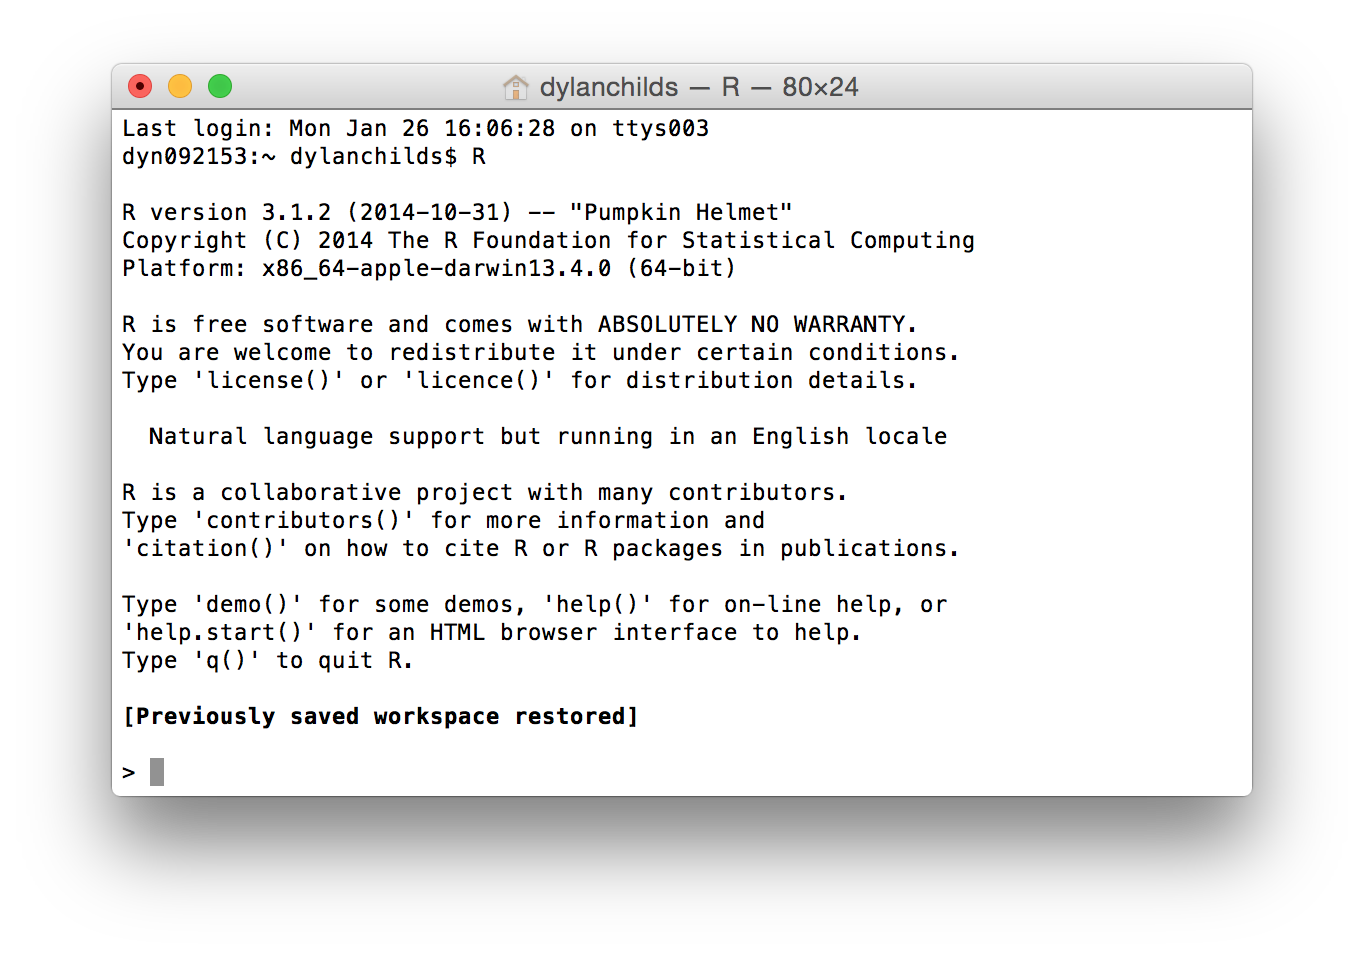
\includegraphics{images/R-terminal.png}

We can run R in much the same way on Windows using the ``Command Prompt'' if we need to. The key thing you need to take away from that screenshot is that running R like this is very ``bare bones''. We typed the letter ``R'' in the Terminal and hit Enter to start R. It printed a little information as it started up and then presented us with ``the prompt'' (\texttt{\textgreater{}}), waiting for input. This is where we type or paste in instructions telling R what to do. There is no other way to interact with it when we run R like this -- no menus or buttons, just a lonely prompt waiting for instructions.

So what is RStudio? In one sense RStudio is just another Graphical User Interface for R which improves on the ``bare bones'' experience. However, it is a GUI on steroids. It is more accurate to describe it as an \href{http://en.wikipedia.org/wiki/Integrated_development_environment}{Integrated Development Environment} (IDE). There is no all-encompassing definition of an IDE, but they all exist to make programmer's lives easier by integrating various useful tools into a single piece of software. From the perspective of this book, there are four key features that we care about:

\begin{itemize}
\item
  The R interpreter---the thing that was running in the Terminal above---runs inside RStudio. It's accessed via a window labelled Console. This is where we type in instructions we want to execute when we are working directly with R. The Console also shows us any output that R prints in response to these instructions. So if we just want the ``bare bones'' experience, we can still have it.
\item
  RStudio provides facilities for working with R programs using something called a Source Code Editor. An R program ( also called a ``script'')" is just is a collection of instructions in the R language that have been saved to a text file. Nothing more! However, it is much easier to work with a script using a proper Source Code Editor than an ordinary text editor like Notepad.
\item
  An good IDE like RStudio also gives you a visual, point-and-click means of accessing various language-specific features. This is a bit difficult to explain until we have have actually used some of these, but trust us, being able to do things like manage packages, set working directories, or inspect objects we've made simplifies day-to-day use of R. This especially true for new users.
\item
  RStudio is cross-platform---it will run on a Windows PC, a Linux PC or a Mac. In terms of the appearance and the functionality it provides, RStudio is exactly the same on each of these platforms. If we learn to work with R via RStudio on a Windows PC, it's no problem migrating to a Mac or Linux PC later on if we need to. This is a big advantage for those of us who work on multiple platforms.
\end{itemize}

We'll only scratch the surface of what RStudio can do. The reason for introducing a powerful tool like RStudio is because one day you may need to access sophisticated features like debugging facilities, package build tools, and repository management. RStudio makes it easy to use these advanced tools.

\hypertarget{how-to-use-this-book}{%
\chapter*{How to use this book}\label{how-to-use-this-book}}
\addcontentsline{toc}{chapter}{How to use this book}

We have adopted a number of formatting conventions in this book to distinguish between normal text, R code, file names, and so on. You need to be aware to make best use of the book.

\hypertarget{text-instructions-and-explanations}{%
\section*{Text, instructions, and explanations}\label{text-instructions-and-explanations}}
\addcontentsline{toc}{section}{Text, instructions, and explanations}

Normal text---instructions, explanations and so on---are written in the same type as this document. We will tend to use bold for emphasis and italics to highlight specific technical terms when they are first introduced. In addition:

\begin{itemize}
\tightlist
\item
  \texttt{This\ typeface} is used to distinguish R code within a sentence of text: e.g.~``We use the \texttt{mutate} function to change or add new variables.''
\item
  A sequence of selections from an RStudio menu is indicated as follows: e.g.~\textbf{File ▶ New File ▶ R Script}
\item
  File names referred to in general text are given in upper case in the normal typeface: e.g.~MYFILE.CSV.
\end{itemize}

At various points in the text you will come across text in different coloured boxes. These are designed to highlight stand-alone exercises or little pieces of supplementary information that might otherwise break the flow. There are three different kinds of boxes:

\begin{infobox}{action}

\hypertarget{action}{%
\subsubsection*{Action!}\label{action}}
\addcontentsline{toc}{subsubsection}{Action!}

This is an \textbf{action} box. We use these when we want you to do something. Do not ignore these boxes.

\end{infobox}

\begin{infobox}{information}

\hypertarget{information}{%
\subsubsection*{Information!}\label{information}}
\addcontentsline{toc}{subsubsection}{Information!}

This is an \textbf{information} box. These aim to offer a discussion of why something works the way it does.

\end{infobox}

\begin{infobox}{warning}

\hypertarget{warning}{%
\subsubsection*{Warning!}\label{warning}}
\addcontentsline{toc}{subsubsection}{Warning!}

This is a \textbf{warning} box. These usually highlight a common `gotcha' that might trip up new users.

\end{infobox}

\hypertarget{r-code-and-output}{%
\section*{R code and output}\label{r-code-and-output}}
\addcontentsline{toc}{section}{R code and output}

We try to illustrate ideas using snippets of real R code where possible. It's a good idea to run these when working through a topic. The best way to learn something is to use it. Of course, in order to do that we need to know what we're looking at\ldots{} Stand alone snippets will be formatted like this:

\begin{Shaded}
\begin{Highlighting}[]
\NormalTok{tmp }\OtherTok{\textless{}{-}} \DecValTok{1}
\FunctionTok{print}\NormalTok{(tmp)}
\end{Highlighting}
\end{Shaded}

\begin{verbatim}
## [1] 1
\end{verbatim}

At this point it does not matter what the above actually means. You just need to understand how the formatting of R code in this book works. The lines that start with \texttt{\#\#} show us what R prints to the screen after it evaluates an instruction and does whatever was asked of it, that is, they show the output. The lines that \textbf{do not} start with \texttt{\#\#} show us the instructions, that is, they show us the input. So remember, the absence of \texttt{\#\#} shows us what we are asking R to do, otherwise we are looking at something R prints in response to these instructions.

\hypertarget{get-up-and-running}{%
\chapter*{Get up and running}\label{get-up-and-running}}
\addcontentsline{toc}{chapter}{Get up and running}

\hypertarget{different-ways-to-run-rstudio}{%
\section*{Different ways to run RStudio}\label{different-ways-to-run-rstudio}}
\addcontentsline{toc}{section}{Different ways to run RStudio}

We can run RStudio in a variety of different ways---

\begin{enumerate}
\def\labelenumi{\arabic{enumi}.}
\tightlist
\item
  Most people use the version of RStudio called \textbf{RStudio Desktop}, either in its free-to-use guise (Open Source Edition) or the commercial version (RStudio Desktop Pro). The desktop version of RStudio are stand-alone applications that run locally on a computer and have to be installed like any other piece of software. This is generally easy, but you can run into problems if you have an old computer or a Chromebook.
\item
  The second way to use RStudio is by accessing a version called \textbf{RStudio Server} through a web browser. RStudio Server is usually administered by professional IT people. Life is easy if you belong to an organisation that has set up RStudio Server, because all you need to get going is a user account, a semi-modern web browser and an internet connection.
\item
  Finally, the company that makes RStudio also runs a commercial cloud-based solution called \href{https://rstudio.com/products/cloud/}{RStudio Cloud}. This allows anyone web browser and an internet connection to use R and RStudio. Although there is a free version, this is fairly limited meaning you end up paying a monthly fee to do `real work'. However, RStudio Cloud can be a good backup option when all else fails.
\end{enumerate}

\begin{infobox}{information}

\hypertarget{do-you-need-to-install-r-and-rstudio}{%
\subsubsection*{Do you need to install R and RStudio?}\label{do-you-need-to-install-r-and-rstudio}}
\addcontentsline{toc}{subsubsection}{Do you need to install R and RStudio?}

If you're lucky enough to have access to RStudio Server or an RStudio Cloud account you don't need to install R and RStudio on your own computer. Just access those cloud service through a decent web browser. That said, it can be useful to have a local copy on your own computer, e.g.~because you don't have a reliable internet connection. Obviously, if you can't access those cloud services you'll have to install R and RStudio to use them!

\end{infobox}

\hypertarget{installing-r-and-rstudio-locally}{%
\section*{Installing R and RStudio locally}\label{installing-r-and-rstudio-locally}}
\addcontentsline{toc}{section}{Installing R and RStudio locally}

It does not need to cost a penny to use R and RStudio. The source code for R is open source, meaning anyone with the time, energy and expertise is free to download it and alter it as they please. Open source does not necessarily mean free, as in it costs £0 to use, but luckily R \textbf{is} free in this sense. On the other hand, RStudio is developed and maintained by a for-profit company (called\ldots{} RStudio). Luckily, because they make their money selling professional software and services, the open source desktop version of RStudio is also free to use. This section will show you how to download and install R and RStudio.

\hypertarget{installing-r}{%
\subsubsection*{Installing R}\label{installing-r}}
\addcontentsline{toc}{subsubsection}{Installing R}

In order to install R you need to download the appropriate installer from the Comprehensive R Archive Network (\href{http://cran.r-project.org}{CRAN}). We are going to use the ``base distribution'' as this contains everything you need to use R under normal circumstances. There is a single \href{http://cran.r-project.org/bin/windows/base/}{installer} for Windows. On a Mac, it's important to match the \href{http://cran.r-project.org/bin/macosx/}{installer} to the version of OS X. In either case, R uses a the standard install mechanism that should be familiar to anyone who has installed an application on their machine. There is no need to change the default settings---doing so will probably lead to problems later on.

After installing R it should be visible in the Programs menu on a Windows computer or in the Applications folder on a Mac. In fact, that thing labelled `R' is very simple a \href{http://en.wikipedia.org/wiki/Graphical_user_interface}{Graphical User Interface} (GUI) for R. When we launch the R GUI we're presented with something called the Console, which is where we can interact directly with R by typing things at the so-called prompt, \texttt{\textgreater{}}, and a few buttons and menus for managing common tasks. We will not study the GUIs in any detail because we recommend using RStudio, but it's important to be aware they exist so that you don't accidentally use them instead of RStudio.

\hypertarget{installing-rstudio}{%
\subsection*{Installing RStudio}\label{installing-rstudio}}
\addcontentsline{toc}{subsection}{Installing RStudio}

RStudio can be downloaded from the RStudio \href{http://www.rstudio.com/products/RStudio/\#Desk}{download page}. The one to go for is the Open Source Edition of RStudio Desktop, \textbf{not} the commercial version of RStudio Desktop called RStudio Desktop Pro. RStudio installs like any other piece of software---just run the installer and follow the instructions. There's no need to configure after after installation.

\hypertarget{a-quick-look-at-rstudio}{%
\section*{A quick look at RStudio}\label{a-quick-look-at-rstudio}}
\addcontentsline{toc}{section}{A quick look at RStudio}

Once installed RStudio runs like any other stand-alone application via the Programs menu or the Applications folder on a Windows PC or Mac, respectively (though it will only work properly if R is also installed). Here is how RStudio appears the first time it runs on a Mac:

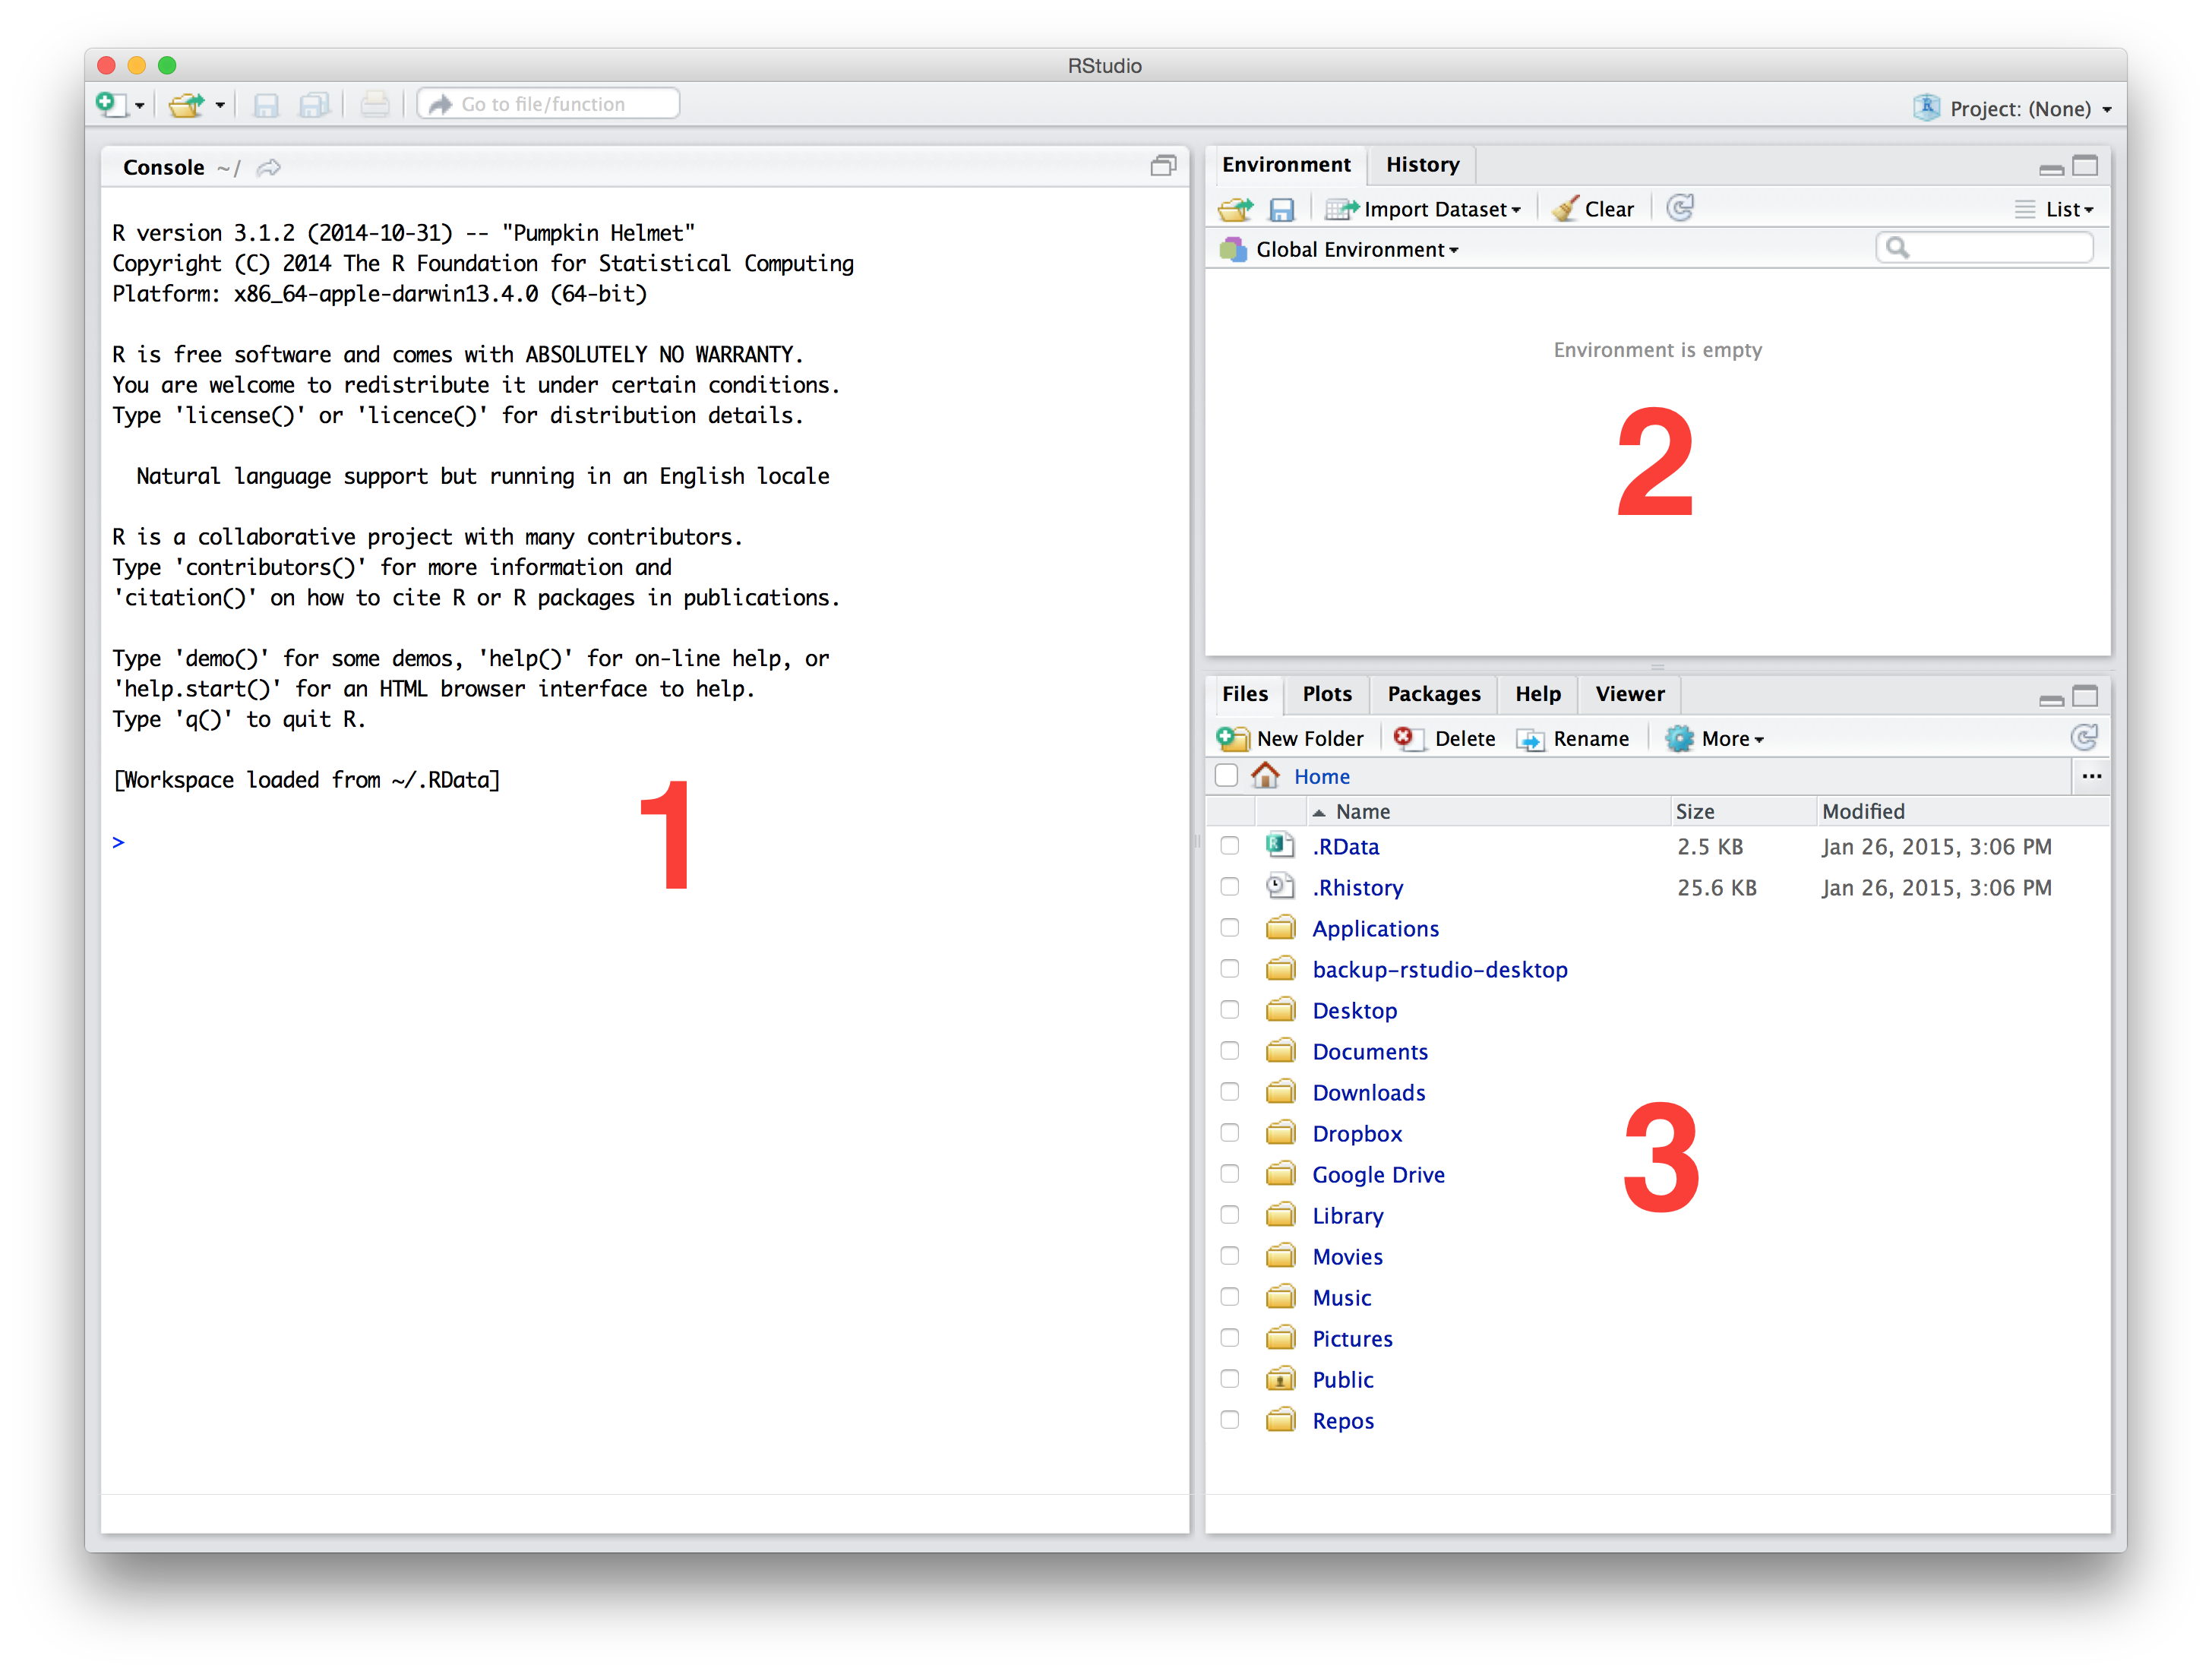
\includegraphics{images/RStudio-3-pane.png}

There are three panes inside a single window, which we have labelled with red numbers. Each of these has a well-defined purpose. Let's take a quick look at these:

\begin{enumerate}
\def\labelenumi{\arabic{enumi}.}
\item
  The large window on the left is the Console. This is basically where R lives inside RStudio. The Console lets you know what R is doing and provides a mechanism to interact with R by typing instructions. All this happens at the prompt, \texttt{\textgreater{}}. You will be working in the Console in the next chapter so we won't say any more about this here.
\item
  The window at the top right contains two or more tabs. One of these, labelled \textbf{Environment}, allows us to see all the R `objects' we can currently access. Another, labelled \textbf{History}, allows us to see a list of instructions we've previously sent to R. The buttons in this tab allow us to reuse or save these instructions.
\item
  The window at the bottom right contains five tabs. The first, labelled \textbf{Files}, gives us a way to interact with the files and folders. The next tab, labelled \textbf{Plots}, is where any figures we produce are displayed. This tab also allows you to save your figures to file. The \textbf{Packages} tab is where we view, install and update packages used to extend the functionality of R. The \textbf{Help} tab is where you can access and display various different help pages. Finally, \textbf{Viewer} is an embedded web browser.
\end{enumerate}

\begin{infobox}{information}

\hypertarget{my-rstudio-looks-different}{%
\subsubsection*{My RStudio looks different!}\label{my-rstudio-looks-different}}
\addcontentsline{toc}{subsubsection}{My RStudio looks different!}

Don't be alarmed if RStudio looks different on your computer. RStudio saves its state between different sessions, so if you've have already messed about with it you will see these changes when you restart it. For example, there is a fourth pane that is often be visible in RStudio---the source code Editor we mentioned above.

\end{infobox}

\hypertarget{working-at-console}{%
\section*{Working at the Console in RStudio}\label{working-at-console}}
\addcontentsline{toc}{section}{Working at the Console in RStudio}

R was designed to be used interactively---it is what is known as an \textbf{interpreted language}, which we can interact with via something called a Command Line Interface (CLI). This is just a fancy way of saying that we can type instructions to ``do something'' into the Console and those instructions will then be interpreted when we hit the Enter key. If our R instructions do not contain any errors, R will then do something like read in some data, perform a calculation, make a figure, and so on. What actually happens obviously depends on what we ask it to do.

Let's briefly see what all this means by doing something very simple with R. Type \texttt{1\ +\ 3} at the Console and hit the Enter key:

\begin{Shaded}
\begin{Highlighting}[]
\DecValTok{1}\SpecialCharTok{+}\DecValTok{3}
\end{Highlighting}
\end{Shaded}

\begin{verbatim}
## [1] 4
\end{verbatim}

The first line above just reminds us what we typed into the Console. The line after that beginning with \texttt{\#\#} shows us what R printed to the Console after reading and evaluating our instructions.

What just happened? We can ignore the \texttt{{[}1{]}} bit for now (the meaning of this will become clear later in the course). What are we left with -- the number 4. The instruction we gave R was in effect ``evaluate the expression \texttt{1\ +\ 3}''. R read this in, decided it was a valid R expression, evaluated the expression, and then printed the result to the Console for us. Unsurprisingly, the expression \texttt{1\ +\ 3} is a request to add the numbers 1 and 3, and so R prints the number 4 to the Console.

OK\ldots{} that was not very exciting. In the next chapter we will start learning to use R to carry out more useful calculations. The important take-away from this is that this sequence of events---reading instructions, evaluating those instructions and printing their output (if there is any output)---happens every time we type or paste something into the Console and hit Enter.

\begin{infobox}{information}

\hypertarget{what-does-that-word-expression-mean}{%
\subsubsection*{What does that word `expression' mean?}\label{what-does-that-word-expression-mean}}
\addcontentsline{toc}{subsubsection}{What does that word `expression' mean?}

Why do we keep using that word \emph{expression}? Here is what the \href{http://en.wikipedia.org/wiki/Expression_(computer_science)}{Wikipedia page} says:

\begin{quote}
An expression in a programming language is a combination of explicit values, constants, variables, operators, and functions that are interpreted according to the particular rules of precedence and of association for a particular programming language, which computes and then produces another value.
\end{quote}

That probably doesn't make much sense! In simple terms, an R expression is a small set of instructions that tell R to do something. That's it. We could write `instructions' instead of `expressions' throughout this book but we may as well use the correct word.

\end{infobox}

\hypertarget{part-introduction-to-r}{%
\part{Introduction to R}\label{part-introduction-to-r}}

\hypertarget{quick-intro-to-r}{%
\chapter{A quick introduction to R}\label{quick-intro-to-r}}

\hypertarget{r-calculator}{%
\section{Using R as a big calculator}\label{r-calculator}}

\hypertarget{basic-arithmetic}{%
\subsection{Basic arithmetic}\label{basic-arithmetic}}

The \protect\hyperlink{working-at-console}{Get up and running chapter} showed that R could handle familiar arithmetic operations: division, multiplication, addition and subtraction. If we want to add or subtract two numbers, we place the \texttt{+} or \texttt{-} symbol in between two numbers and hit Enter. R will read the arithmetic expression, evaluate it, and print the result to the Console. This works as you'd expect:

\emph{Addition}--

\begin{Shaded}
\begin{Highlighting}[]
\DecValTok{3} \SpecialCharTok{+} \DecValTok{2}
\end{Highlighting}
\end{Shaded}

\begin{verbatim}
## [1] 5
\end{verbatim}

\emph{Subtraction}--

\begin{Shaded}
\begin{Highlighting}[]
\DecValTok{5} \SpecialCharTok{{-}} \DecValTok{1}
\end{Highlighting}
\end{Shaded}

\begin{verbatim}
## [1] 4
\end{verbatim}

Multiplication and division are no different. However, we can't use \texttt{x} or \texttt{÷} symbols for these operations. Instead, use \texttt{*} and \texttt{/} to multiply and divide:

\emph{Multiplication}--

\begin{Shaded}
\begin{Highlighting}[]
\DecValTok{7} \SpecialCharTok{*} \DecValTok{2}
\end{Highlighting}
\end{Shaded}

\begin{verbatim}
## [1] 14
\end{verbatim}

\emph{Division}--

\begin{Shaded}
\begin{Highlighting}[]
\DecValTok{3} \SpecialCharTok{/} \DecValTok{2}
\end{Highlighting}
\end{Shaded}

\begin{verbatim}
## [1] 1.5
\end{verbatim}

We can also exponentiate numbers, i.e.~raise one number to the power of another. Use the \texttt{\^{}} operator to do this:

\emph{Exponentiation}--

\begin{Shaded}
\begin{Highlighting}[]
\DecValTok{4}\SpecialCharTok{\^{}}\DecValTok{2}
\end{Highlighting}
\end{Shaded}

\begin{verbatim}
## [1] 16
\end{verbatim}

This raises 4 to the power of 2 (i.e.~we squared it). In general, we can raise a number \texttt{x} to the power of \texttt{y} using \texttt{x\^{}y}. Neither \texttt{x} nor \texttt{y} need to be whole numbers either.

\begin{infobox}{information}

\hypertarget{operators}{%
\subsubsection*{Operators?}\label{operators}}
\addcontentsline{toc}{subsubsection}{Operators?}

What does `operator' mean? An operator is simply a symbol (or sequence of symbols) that does something specific with one or more inputs. For example, operators like \texttt{/}, \texttt{*}, \texttt{+} and \texttt{-} carry out arithmetic calculations with pairs of numbers. Operators are one of the basic building blocks of a programming language like R.

\end{infobox}

\hypertarget{combining-arithmetic-operations}{%
\subsection{Combining arithmetic operations}\label{combining-arithmetic-operations}}

We can also combine arithmetic operations. Assume we want to subtract 6 from 2\textsuperscript{3}. The expression to perform this calculation is:

\begin{Shaded}
\begin{Highlighting}[]
\DecValTok{2}\SpecialCharTok{\^{}}\DecValTok{3} \SpecialCharTok{{-}} \DecValTok{6}
\end{Highlighting}
\end{Shaded}

\begin{verbatim}
## [1] 2
\end{verbatim}

Simple enough, but what if we had wanted to carry out a slightly longer calculation that required the last answer to then be divided by 2? This is the \textbf{wrong} way to do this:

\begin{Shaded}
\begin{Highlighting}[]
\DecValTok{2}\SpecialCharTok{\^{}}\DecValTok{3} \SpecialCharTok{{-}} \DecValTok{6} \SpecialCharTok{/} \DecValTok{2}
\end{Highlighting}
\end{Shaded}

\begin{verbatim}
## [1] 5
\end{verbatim}

The answer we expect here is \(1\). So what happened? R evaluated \(6/2\) first and then subtracted this answer from \(2^3\).

If that's obvious, great. If not, it's time to learn about \textbf{order of precedence}. R uses a standard set of rules to decide the order in which calculations feed into one another to unambiguously evaluate any expression. It uses the same order as every other computer language, which thankfully is the same one we all learn in mathematics classes at school. The order of precedence is:

\begin{enumerate}
\def\labelenumi{\arabic{enumi}.}
\item
  exponents and roots (also, `powers' or `orders')
\item
  division and then multiplication
\item
  additional and then subtraction
\end{enumerate}

\begin{infobox}{information}

\hypertarget{bodmas-and-friends}{%
\subsubsection*{BODMAS and friends}\label{bodmas-and-friends}}
\addcontentsline{toc}{subsubsection}{BODMAS and friends}

If you find it difficult to remember the standard order of precedence there are a load of \href{http://en.wikipedia.org/wiki/Order_of_operations\#Mnemonics}{mnemonics} that can to help.

\end{infobox}

We need to control the order of evaluation to arrive at the answer we were looking for in the above example. Do this by grouping together calculations inside parentheses, i.e.~`round brackets' \texttt{(} and \texttt{)}. Here's the expression we should have used:

\begin{Shaded}
\begin{Highlighting}[]
\NormalTok{(}\DecValTok{2}\SpecialCharTok{\^{}}\DecValTok{3} \SpecialCharTok{{-}} \DecValTok{6}\NormalTok{) }\SpecialCharTok{/} \DecValTok{2}
\end{Highlighting}
\end{Shaded}

\begin{verbatim}
## [1] 1
\end{verbatim}

We can use more than one pair of parentheses to control the order of evaluation in more complex calculations. The order of evaluation then happens `inside-out'. For example, if we want to find the cube root of 2 (i.e.~2\textsuperscript{1/3}) rather than 2\textsuperscript{3} in that last calculation we would instead write:

\begin{Shaded}
\begin{Highlighting}[]
\NormalTok{(}\DecValTok{2}\SpecialCharTok{\^{}}\NormalTok{(}\DecValTok{1}\SpecialCharTok{/}\DecValTok{3}\NormalTok{) }\SpecialCharTok{{-}} \DecValTok{6}\NormalTok{) }\SpecialCharTok{/} \DecValTok{2}
\end{Highlighting}
\end{Shaded}

\begin{verbatim}
## [1] -2.370039
\end{verbatim}

The parentheses around the \texttt{1/3} are needed to ensure this is evaluated prior to being used as the exponent.

\begin{infobox}{action}

\hypertarget{working-efficiently-at-the-console}{%
\subsubsection*{Working efficiently at the Console}\label{working-efficiently-at-the-console}}
\addcontentsline{toc}{subsubsection}{Working efficiently at the Console}

Working at the Console soon gets tedious if we have to retype similar things over and over again. There is no need to do this, though. Place the cursor at the prompt and hit the up arrow. What happens? This brings back the last expression sent to R's interpreter. Hit the up arrow again to see the last-but-one expression, and so on. We go back down the list using the down arrow. Once we're at the line we need, we use the left and right arrows to move around the expression and the delete key to remove the parts we want to change. Once an expression has been edited we can hit Enter to send it to R again. Try it.

\end{infobox}

\hypertarget{problematic-calculations}{%
\section{Problematic calculations}\label{problematic-calculations}}

Now is a good time to highlight how R handles certain kinds of awkward numerical calculations. One of these involves division of a non-zero by 0. Mathematically, division of a finite number by \texttt{0} equals A Very Large Number: infinity. Some programming languages will respond to an attempt to do this with an error. R is a bit more forgiving:

\begin{Shaded}
\begin{Highlighting}[]
\DecValTok{1} \SpecialCharTok{/} \DecValTok{0}
\end{Highlighting}
\end{Shaded}

\begin{verbatim}
## [1] Inf
\end{verbatim}

R has a special built-in value that allows it to handle this kind of result. This is \texttt{Inf}, which stands for `infinity'.

The other special kind of value we sometimes run into is generated by calculations that don't have a well-defined numerical result. For example, look what happens when we try to divide 0 by 0:

\begin{Shaded}
\begin{Highlighting}[]
\DecValTok{0} \SpecialCharTok{/} \DecValTok{0}
\end{Highlighting}
\end{Shaded}

\begin{verbatim}
## [1] NaN
\end{verbatim}

The \texttt{NaN} in this result stands for `Not a Number'. R produces \texttt{NaN} because \(0 / 0\) is not defined mathematically: it produces something that is Not a Number.

The reason we are pointing out \texttt{Inf} and \texttt{NaN} is not that we expect to use them. It's important to know what they represent because they often arise due to a mistake somewhere in our code. It's hard to track down such mistakes if we don't know how \texttt{Inf} and \texttt{NaN} arise.

\begin{infobox}{information}

\hypertarget{r-as-a-fancy-calculator}{%
\subsubsection*{R as a fancy calculator}\label{r-as-a-fancy-calculator}}
\addcontentsline{toc}{subsubsection}{R as a fancy calculator}

What we've seen so far is that we can interact with R via the so-called REPL: the read-evaluate-print loop. R takes user input (e.g.~\texttt{1\ /\ 0}), evaluates it (\texttt{1\ /\ 0\ =\ Inf}), prints the results (\texttt{\#\#\ {[}1{]}\ Inf}), and then waits for the next input (e.g.~\texttt{0\ /\ 0}). This facility is handy because it means we can use R interactively, working through a set of calculations line-by-line.

\end{infobox}

\hypertarget{assignment}{%
\section{Storing and reusing results}\label{assignment}}

We've not yet tried to do anything remotely complicated or interesting beyond using parentheses to construct longer calculations. This approach is acceptable when a calculation is straightforward, but it quickly becomes unwieldy for dealing with anything more complicated.

The best way to see what we mean is by working through a simple example---solving a quadratic equation. You probably remember these from school. A quadratic equation looks like this:

\[a + bx + cx^2 = 0\] If we know the values of \(a\), \(b\) and \(c\) then we can solve this equation to find the values of \(x\) that satisfy this equation. Here's the well-known formula for these solutions: \[
x = \frac{-b\pm\sqrt{b^2-4ac}}{2a}
\] We can use R to calculate these solutions for us. Say that we want to find the solutions to the quadratic equation when \(a=1\), \(b=6\) and \(c=5\). We have to turn the above equation into a pair of R expressions:

\emph{Solution 1}--

\begin{Shaded}
\begin{Highlighting}[]
\NormalTok{(}\SpecialCharTok{{-}}\DecValTok{6} \SpecialCharTok{+}\NormalTok{ (}\DecValTok{6}\SpecialCharTok{\^{}}\DecValTok{2} \SpecialCharTok{{-}}\DecValTok{4} \SpecialCharTok{*} \DecValTok{1} \SpecialCharTok{*} \DecValTok{5}\NormalTok{)}\SpecialCharTok{\^{}}\NormalTok{(}\DecValTok{1}\SpecialCharTok{/}\DecValTok{2}\NormalTok{)) }\SpecialCharTok{/}\NormalTok{ (}\DecValTok{2} \SpecialCharTok{*} \DecValTok{1}\NormalTok{)}
\end{Highlighting}
\end{Shaded}

\begin{verbatim}
## [1] -1
\end{verbatim}

\emph{Solution 2}--

\begin{Shaded}
\begin{Highlighting}[]
\NormalTok{(}\SpecialCharTok{{-}}\DecValTok{6} \SpecialCharTok{{-}}\NormalTok{ (}\DecValTok{6}\SpecialCharTok{\^{}}\DecValTok{2} \SpecialCharTok{{-}}\DecValTok{4} \SpecialCharTok{*} \DecValTok{1} \SpecialCharTok{*} \DecValTok{5}\NormalTok{)}\SpecialCharTok{\^{}}\NormalTok{(}\DecValTok{1}\SpecialCharTok{/}\DecValTok{2}\NormalTok{)) }\SpecialCharTok{/}\NormalTok{ (}\DecValTok{2} \SpecialCharTok{*} \DecValTok{1}\NormalTok{)}
\end{Highlighting}
\end{Shaded}

\begin{verbatim}
## [1] -5
\end{verbatim}

The output tells us that the two values of \(x\) that satisfy this particular quadratic equation are -1 and -5.

But what should we do if we now need to solve a different quadratic equation? Working at the Console, we could bring up the expressions we typed (using the up arrow) and change the numbers to match the new values of \(a\), \(b\) and \(c\). However, editing expressions like this is tedious, and more importantly, it's error-prone because we have to make sure we substitute the new numbers into precisely the right positions.

A partial solution to this problem is to store the values of \(a\), \(b\) and \(c\) in some way so that we only have to change them one. We'll see why this is useful in a moment.

First, we need to learn how to store results in R. The key to this is to use the \textbf{assignment operator}, written as an arrow pointing to the left, \texttt{\textless{}-}. Sticking with the current example, we need to store the numbers 1, 6 and 5. We do this by typing out three expressions, one after the another, each time hitting enter to get R to evaluate it:

\begin{Shaded}
\begin{Highlighting}[]
\NormalTok{a }\OtherTok{\textless{}{-}} \DecValTok{1}
\end{Highlighting}
\end{Shaded}

\begin{Shaded}
\begin{Highlighting}[]
\NormalTok{b }\OtherTok{\textless{}{-}} \DecValTok{6}
\end{Highlighting}
\end{Shaded}

\begin{Shaded}
\begin{Highlighting}[]
\NormalTok{c }\OtherTok{\textless{}{-}} \DecValTok{5}
\end{Highlighting}
\end{Shaded}

The exact sequence \texttt{\textless{}-} defines the assignment operator. R won't recognise it as assignment if we try to include a space between the \texttt{\textless{}} and \texttt{-} symbols.

Notice that R didn't print anything to screen. So what actually happened? We asked R to first evaluate the expression on the right hand side of each \texttt{\textless{}-} (just a number in this case) and then \textbf{assigns the result} of that evaluation instead of printing it. Each result has a name associated with it, which appears on the left hand-side of the \texttt{\textless{}-}.

The net result of all this is that we have stored the numbers 1, 6 and 5 somewhere in R and associated them with the letters \texttt{a}, \texttt{b} and \texttt{c}, respectively. We can check whether this assignment business has worked by looking at the \textbf{Environment} tab in the top right RStudio window. There should be three `names' listed in that tab now (\texttt{a}, \texttt{b} and \texttt{c}) along with the associated numbers 1, 6 and 5.

What does this mean in practical terms? Look at what happens if we now type the letter \texttt{a} into the Console and hit Enter:

\begin{Shaded}
\begin{Highlighting}[]
\NormalTok{a}
\end{Highlighting}
\end{Shaded}

\begin{verbatim}
## [1] 1
\end{verbatim}

It looks the same as if we had typed the number \texttt{1} directly into the Console. We stored the output from three separate R expressions, associating each a name so that we can access it again\footnote{Technically, this is called \textbf{binding} the name to a value. You don't need to remember this.}. Whenever we use the assignment operator \texttt{\textless{}-} we are telling R to keep whatever kind of value results from the calculation on the right-hand side of \texttt{\textless{}-}, giving it the name on the left-hand side so that we can access it later.

Why is this useful? Let's imagine we want to do more than one thing with our three numbers. If we want to know their sum or their product we can now use:

\emph{Sum}--

\begin{Shaded}
\begin{Highlighting}[]
\NormalTok{a }\SpecialCharTok{+}\NormalTok{ b }\SpecialCharTok{+}\NormalTok{ c}
\end{Highlighting}
\end{Shaded}

\begin{verbatim}
## [1] 12
\end{verbatim}

\emph{Product}--

\begin{Shaded}
\begin{Highlighting}[]
\NormalTok{a }\SpecialCharTok{*}\NormalTok{ b }\SpecialCharTok{*}\NormalTok{ c}
\end{Highlighting}
\end{Shaded}

\begin{verbatim}
## [1] 30
\end{verbatim}

So\ldots{} once we've stored a result and associated it with a name we can reuse it whenever needed. Returning to our example, we can now calculate the solutions to the quadratic equation by typing these two expressions into the Console:

\emph{Solution 1}--

\begin{Shaded}
\begin{Highlighting}[]
\NormalTok{(}\SpecialCharTok{{-}}\NormalTok{b }\SpecialCharTok{+}\NormalTok{ (b}\SpecialCharTok{\^{}}\DecValTok{2} \SpecialCharTok{{-}}\DecValTok{4} \SpecialCharTok{*}\NormalTok{ a }\SpecialCharTok{*}\NormalTok{ c)}\SpecialCharTok{\^{}}\NormalTok{(}\DecValTok{1}\SpecialCharTok{/}\DecValTok{2}\NormalTok{)) }\SpecialCharTok{/}\NormalTok{ (}\DecValTok{2} \SpecialCharTok{*}\NormalTok{ a)}
\end{Highlighting}
\end{Shaded}

\begin{verbatim}
## [1] -1
\end{verbatim}

\emph{Solution 2}--

\begin{Shaded}
\begin{Highlighting}[]
\NormalTok{(}\SpecialCharTok{{-}}\NormalTok{b }\SpecialCharTok{{-}}\NormalTok{ (b}\SpecialCharTok{\^{}}\DecValTok{2} \SpecialCharTok{{-}}\DecValTok{4} \SpecialCharTok{*}\NormalTok{ a }\SpecialCharTok{*}\NormalTok{ c)}\SpecialCharTok{\^{}}\NormalTok{(}\DecValTok{1}\SpecialCharTok{/}\DecValTok{2}\NormalTok{)) }\SpecialCharTok{/}\NormalTok{ (}\DecValTok{2} \SpecialCharTok{*}\NormalTok{ a)}
\end{Highlighting}
\end{Shaded}

\begin{verbatim}
## [1] -5
\end{verbatim}

Imagine we'd now like to find the solutions to a different quadratic equation where \(a=1\), \(b=5\) and \(c=5\). We only changed the value of \(b\) here. To find the new solutions we have to do two things. First we change the value of the number associated with \texttt{b}\ldots{}

\begin{Shaded}
\begin{Highlighting}[]
\NormalTok{b }\OtherTok{\textless{}{-}} \DecValTok{5}
\end{Highlighting}
\end{Shaded}

\ldots then we bring up those lines that calculate the solutions to the quadratic equation and run them, one after the other:

\begin{Shaded}
\begin{Highlighting}[]
\NormalTok{(}\SpecialCharTok{{-}}\NormalTok{b }\SpecialCharTok{+}\NormalTok{ (b}\SpecialCharTok{\^{}}\DecValTok{2} \SpecialCharTok{{-}}\DecValTok{4} \SpecialCharTok{*}\NormalTok{ a }\SpecialCharTok{*}\NormalTok{ c)}\SpecialCharTok{\^{}}\NormalTok{(}\DecValTok{1}\SpecialCharTok{/}\DecValTok{2}\NormalTok{)) }\SpecialCharTok{/}\NormalTok{ (}\DecValTok{2} \SpecialCharTok{*}\NormalTok{ a)}
\end{Highlighting}
\end{Shaded}

\begin{verbatim}
## [1] -1.381966
\end{verbatim}

\begin{Shaded}
\begin{Highlighting}[]
\NormalTok{(}\SpecialCharTok{{-}}\NormalTok{b }\SpecialCharTok{{-}}\NormalTok{ (b}\SpecialCharTok{\^{}}\DecValTok{2} \SpecialCharTok{{-}}\DecValTok{4} \SpecialCharTok{*}\NormalTok{ a }\SpecialCharTok{*}\NormalTok{ c)}\SpecialCharTok{\^{}}\NormalTok{(}\DecValTok{1}\SpecialCharTok{/}\DecValTok{2}\NormalTok{)) }\SpecialCharTok{/}\NormalTok{ (}\DecValTok{2} \SpecialCharTok{*}\NormalTok{ a)}
\end{Highlighting}
\end{Shaded}

\begin{verbatim}
## [1] -3.618034
\end{verbatim}

We don't have to retype those expressions. We can use the up arrow to bring each one back to the prompt and hit Enter. This is much simpler than editing the expressions.

More importantly, we are beginning to see the benefits of using something like R---we can break down complex calculations into a series of steps, storing and reusing intermediate results as required.

\begin{infobox}{action}

\hypertarget{rstudio-shortcut}{%
\subsubsection*{RStudio shortcut}\label{rstudio-shortcut}}
\addcontentsline{toc}{subsubsection}{RStudio shortcut}

We use the assignment operator \texttt{\textless{}-} all the time when working with R. Because it's inefficient to type the \texttt{\textless{}} and \texttt{-} characters repeatedly, RStudio has a built-in shortcut for typing the assignment operator.

The shortcut is `Alt + \texttt{-}' . Try it now. Move the cursor to the Console, hold down the Alt key (`Option' on a Mac), and press the \texttt{-} sign key. RStudio will auto-magically add insert \texttt{\textless{}-}. \textbf{If you only learn one RStudio shortcut, learn this one!} It will save you a lot of time in the long run.

\end{infobox}

\hypertarget{how-does-assignment-work}{%
\section{How does assignment work?}\label{how-does-assignment-work}}

When we use the assignment operator \texttt{\textless{}-} to associate names and values, we refer to this as creating or modifying \textbf{a variable}. This is much less tedious than using words like `associate', `value', and `name' all the time. Why is it called a variable? What happens when we run these lines:

\emph{Create} \texttt{myvar} \emph{and print out its value}--

\begin{Shaded}
\begin{Highlighting}[]
\NormalTok{myvar }\OtherTok{\textless{}{-}} \DecValTok{1}
\NormalTok{myvar}
\end{Highlighting}
\end{Shaded}

\begin{verbatim}
## [1] 1
\end{verbatim}

\emph{Modify} \texttt{myvar} and \emph{and print out its new value} --

\begin{Shaded}
\begin{Highlighting}[]
\NormalTok{myvar }\OtherTok{\textless{}{-}} \DecValTok{7}
\NormalTok{myvar}
\end{Highlighting}
\end{Shaded}

\begin{verbatim}
## [1] 7
\end{verbatim}

The first time we used \texttt{\textless{}-} with \texttt{myvar} on the left-hand side, we \textbf{created} a variable \texttt{myvar} associated with the value 1. We then printed out the value associated with \texttt{myvar}. The second line \texttt{myvar\ \textless{}-\ 7} \textbf{modified} the value of \texttt{myvar} to be 7 (and printed this out again). This is why we refer to \texttt{myvar} as a variable: we can change its value as we please.

What happened to the old value associated with \texttt{myvar}? In short, it is gone, kaput, lost\ldots{} forever. The moment we assign a new value to \texttt{myvar} the old one is destroyed and can no longer be accessed. Remember this.

Keep in mind that the expression on the right-hand side of \texttt{\textless{}-} can be any kind of calculation and the variable can have any (valid) name we like. For example, if we want to perform the calculation \texttt{(1\ +\ 2\^{}3)\ /\ (2\ +\ 7)} and associate the result with the word \texttt{answer}, we would do this:

\begin{Shaded}
\begin{Highlighting}[]
\NormalTok{answer }\OtherTok{\textless{}{-}}\NormalTok{ (}\DecValTok{1} \SpecialCharTok{+} \DecValTok{2}\SpecialCharTok{\^{}}\DecValTok{3}\NormalTok{) }\SpecialCharTok{/}\NormalTok{ (}\DecValTok{2} \SpecialCharTok{+} \DecValTok{7}\NormalTok{)}
\NormalTok{answer}
\end{Highlighting}
\end{Shaded}

\begin{verbatim}
## [1] 1
\end{verbatim}

Any expression can be used on the right-hand side of the assignment operator as along as it generates an output of some kind. For example, we can create new variables from others:

\begin{Shaded}
\begin{Highlighting}[]
\NormalTok{newvar }\OtherTok{\textless{}{-}} \DecValTok{2} \SpecialCharTok{*}\NormalTok{ answer}
\end{Highlighting}
\end{Shaded}

What happened here? Start at the right-hand side of \texttt{\textless{}-}. The expression on this side contained the variable \texttt{answer} so R went to see if \texttt{answer} actually exists. It does, so it then substituted the value associated with \texttt{answer} into the calculation and assigned the resulting value of 2 to \texttt{newvar}.

Finally, look at what happens if we copy a variable using the assignment operator:

\begin{Shaded}
\begin{Highlighting}[]
\NormalTok{myvar }\OtherTok{\textless{}{-}} \DecValTok{7}
\NormalTok{mycopy }\OtherTok{\textless{}{-}}\NormalTok{ myvar}
\end{Highlighting}
\end{Shaded}

We now have a pair of variables, \texttt{myvar} and \texttt{mycopy}, associated with the number 7. Each of these is associated with a \textbf{different copy} of this number. If we change the value associated with one of these variables it does not change the value of the other, as this shows:

\begin{Shaded}
\begin{Highlighting}[]
\NormalTok{myvar }\OtherTok{\textless{}{-}} \DecValTok{10}
\end{Highlighting}
\end{Shaded}

\begin{Shaded}
\begin{Highlighting}[]
\NormalTok{myvar}
\end{Highlighting}
\end{Shaded}

\begin{verbatim}
## [1] 10
\end{verbatim}

\begin{Shaded}
\begin{Highlighting}[]
\NormalTok{mycopy}
\end{Highlighting}
\end{Shaded}

\begin{verbatim}
## [1] 7
\end{verbatim}

R always behaves like this unless we work hard to alter this behaviour. Remember that---every time we assign one variable to another, we actually make a completely new, independent copy of its associated value. That probably doesn't seem like an obvious or important point, but trust us, it is. It will be critical to remember this behaviour when we start learning how to manipulate data sets.

\hypertarget{global-environment}{%
\section{Global environment}\label{global-environment}}

Whenever we associate a name with a value we create a copy of both these things somewhere in the computer's memory. In R the ``somewhere'' is called an environment. We aren't going to get into a discussion of R's many different kinds of environments---that's an advanced topic well beyond the scope of this book. The one environment we do need to be aware of is the \textbf{Global Environment}.

Whenever we perform an assignment in the Console the variable we create is placed into the Global Environment. The set of variables currently in existence are listed in the \textbf{Environment} tab in RStudio. Take a look. There are two columns in the \textbf{Environment} tab: the first shows the names of the variables, the second summarises their values.

\begin{infobox}{warning}

\hypertarget{the-global-environment-is-temporary}{%
\subsubsection*{The Global Environment is temporary}\label{the-global-environment-is-temporary}}
\addcontentsline{toc}{subsubsection}{The Global Environment is temporary}

By default, R will try to save everything in the Global Environment when we close it down and restore everything when we start the next R session. It does this by writing a copy of the Global Environment to disk. In theory, this means we can close down R, reopen it, and pick things up from where we left off. \textbf{Don't rely on this behaviour!} It just increases the risk of making a mistake.

\end{infobox}

\hypertarget{naming-rules-and-conventions}{%
\section{Naming rules and conventions}\label{naming-rules-and-conventions}}

We don't have to use a single letter to name things in R. We could use the words \texttt{tom}, \texttt{dick} and \texttt{harry} in place of \texttt{a}, \texttt{b} and \texttt{c}. It might be confusing to use them, but \texttt{tom}, \texttt{dick} and \texttt{harry} are all legal names as far as to R is concerned:

\begin{itemize}
\item
  A legal name in R is any sequence of letters, numbers, \texttt{.}, or \texttt{\_}, but the sequence of characters we use must begin with a letter. Both upper and lower case letters are allowed. For example, \texttt{num\_1}, \texttt{num.1}, \texttt{num1}, \texttt{NUM1}, \texttt{myNum1} are all legal names, but \texttt{1num} and \texttt{\_num1} are not because they begin with \texttt{1} and \texttt{\_}.
\item
  R is case sensitive---it treats upper and lower case letters as different characters. This means R treats \texttt{num} and \texttt{Num} as distinct names. Forgetting about case sensitivity is a good way to create errors when using R. Try to remember that.
\end{itemize}

\begin{infobox}{warning}

\hypertarget{dont-begin-a-name-with-.}{%
\subsubsection*{\texorpdfstring{Don't begin a name with \texttt{.}}{Don't begin a name with .}}\label{dont-begin-a-name-with-.}}
\addcontentsline{toc}{subsubsection}{Don't begin a name with \texttt{.}}

We are allowed to begin a name with a \texttt{.}, but this usually is A Bad Idea. Why? Because variable names that begin with \texttt{.} are hidden from view in the Global Environment---the value it refers to exists but it's invisible. This behaviour exists to allow R to create invisible variables that control how it behaves. This is useful, but it isn't really meant to be used by the average user.

\end{infobox}

\hypertarget{using-functions}{%
\chapter{Using functions}\label{using-functions}}

\hypertarget{intro-functions}{%
\section{Introduction}\label{intro-functions}}

Functions are an essential building block of any programming language. The job of a function is to carry out a calculation or computation that would typically require many lines code to do `from scratch'. Functions allow us to reuse common computations while offering some control over the precise details of what happens. To use R effectively---even if our needs are very simple---we need to understand how to use functions. This chapter aims to explain what functions are for, how to use them, and how to avoid mistakes when doing so, without getting lost in the detail of how they work.

\hypertarget{functions-and-arguments}{%
\section{Functions and arguments}\label{functions-and-arguments}}

Functions allow us to reuse a calculation. The best way to see what we mean by this is to see one in action. The \texttt{round} function rounds numbers to a significant number of digits (no surprises there). To use it, we could type this into the Console and hit Enter:

\begin{Shaded}
\begin{Highlighting}[]
\FunctionTok{round}\NormalTok{(}\AttributeTok{x =} \FloatTok{3.141593}\NormalTok{, }\AttributeTok{digits =} \DecValTok{2}\NormalTok{)}
\end{Highlighting}
\end{Shaded}

We have suppressed the output so that we can unpack things a bit first. We rely on the same basic construct every time we use a function. This starts with the name of the function as the prefix. In the example above, the function name is \texttt{round}. After the function name, we need a pair of opening and closing parentheses. This combination of name and parentheses alerts R to fact that we are using a function.

What about the bits inside the parentheses? These are called the \textbf{arguments} of the function. That's a horrible name, but it is the one that everyone uses, so we have to get used to it. Depending on how it was defined, a function can take zero, one, or more arguments. We will discuss this idea in more detail later in this section. In simple terms, the arguments control the behaviour of a function.

We used the \texttt{round} function with two arguments. We supplied each one as a name-value pair separated by a comma. When working with arguments, name-value pairs occur either side of the equals sign (\texttt{=}), with the argument \textbf{name} on the left-hand side and its \textbf{value} on the right-hand side. The name serves to identify which argument we are working with, and the value is the thing that controls what that argument does.

We call the process of associating argument names and values `setting the arguments' of the function (or `supplying the arguments'). Notice the similarity between supplying function arguments and the assignment operation discussed in the last topic. The difference is that name-value pairs are associated with the \texttt{=} symbol when involved in arguments.

\begin{infobox}{warning}

\hypertarget{use-to-assign-arguments}{%
\subsubsection*{\texorpdfstring{Use \texttt{=} to assign arguments}{Use = to assign arguments}}\label{use-to-assign-arguments}}
\addcontentsline{toc}{subsubsection}{Use \texttt{=} to assign arguments}

\textbf{Do not} use the assignment operator \texttt{\textless{}-} inside the parentheses when working with functions. This is a ``trust us'' situation---you will end up in all kinds of difficulty if you do this!

\end{infobox}

The arguments control the behaviour of a function. Our job as users is to set the values of these to get the behaviour we want. However, The function determines arguments we are allowed to use, i.e.~we are not free to choose whatever name we like\footnote{We say ``typically'', because R is a very flexible language and so there are certain exceptions to this simple rule of thumb. For now it is simpler to think of the names as constrained by the particular function we're using. Let's return to th example to see how all this works:}.

\begin{Shaded}
\begin{Highlighting}[]
\FunctionTok{round}\NormalTok{(}\AttributeTok{x =} \FloatTok{3.141593}\NormalTok{, }\AttributeTok{digits =} \DecValTok{2}\NormalTok{)}
\end{Highlighting}
\end{Shaded}

\begin{verbatim}
## [1] 3.14
\end{verbatim}

The \texttt{round} function rounds one or more numeric inputs and rounds these to a particular number of significant digits. The argument that specifies the number(s) to round is \texttt{x}; the second argument, \texttt{digits}, specifies the number of decimal places we require. Based on the supplied values of these arguments, \texttt{3.141593} and \texttt{2}, respectively, the \texttt{round} function spits out a value of \texttt{3.14}, which is then printed to the Console.

What if we had wanted to the answer to 3 significant digits? We would set the \texttt{digits} argument to 3:

\begin{Shaded}
\begin{Highlighting}[]
\FunctionTok{round}\NormalTok{(}\AttributeTok{x =} \FloatTok{3.141593}\NormalTok{, }\AttributeTok{digits =} \DecValTok{3}\NormalTok{)}
\end{Highlighting}
\end{Shaded}

\begin{verbatim}
## [1] 3.142
\end{verbatim}

This illustrates what we mean when we say arguments control the behaviour of the function---\texttt{digits} sets the number of significant digits calculated by \texttt{round}.

\hypertarget{evaluating-arguments-and-returning-results}{%
\section{Evaluating arguments and returning results}\label{evaluating-arguments-and-returning-results}}

Whenever R evaluates a function, we refer to this action as `calling the function'. In our simple example, we called the \texttt{round} function with arguments \texttt{x} and \texttt{digits}. That said, we often just say `use the function' because that is more natural to most users.

Several things happen when we call functions: first they \textbf{evaluate} their arguments, then they perform some action, and finally (optionally) \textbf{return} a value to us. Let's work through what all that means\ldots{}

What do we mean by the word `evaluate'? When we call a function, what typically happens is:

\begin{enumerate}
\def\labelenumi{\arabic{enumi}.}
\tightlist
\item
  the R expression on the right-hand side of an \texttt{=} is evaluated,
\item
  the result is associated with the corresponding argument name, and
\item
  the function does its calculations using the resulting name-value pairs.
\end{enumerate}

To see how the evaluation step works, take a look at a new example using \texttt{round}:

\begin{Shaded}
\begin{Highlighting}[]
\FunctionTok{round}\NormalTok{(}\AttributeTok{x =} \FloatTok{2.3} \SpecialCharTok{+} \FloatTok{1.4}\NormalTok{, }\AttributeTok{digits =} \DecValTok{0}\NormalTok{)}
\end{Highlighting}
\end{Shaded}

\begin{verbatim}
## [1] 4
\end{verbatim}

What happened above is that R evaluated \texttt{2.3\ +\ 1.4}, resulting in the number \texttt{3.7}, which was then associated with the argument \texttt{x}. We set \texttt{digits} to \texttt{0} this time so that \texttt{round} returns a whole number, \texttt{4}.

The important thing to realise is that the expression(s) on the right-hand side of the \texttt{=} can be anything we like. This third example essentially equivalent to the last one:

\begin{Shaded}
\begin{Highlighting}[]
\NormalTok{y }\OtherTok{\textless{}{-}} \FloatTok{2.3} \SpecialCharTok{+} \FloatTok{1.4}
\FunctionTok{round}\NormalTok{(}\AttributeTok{x =}\NormalTok{ y, }\AttributeTok{digits =} \DecValTok{0}\NormalTok{)}
\end{Highlighting}
\end{Shaded}

\begin{verbatim}
## [1] 4
\end{verbatim}

This time we created a new variable called \texttt{y} and supplied this as the value of the \texttt{x} argument. When we use the \texttt{round} function like this, the R interpreter spots that something on the right-hand side of an \texttt{=} is a variable and associates the value of this variable with \texttt{x} argument. As long as we have defined the numeric variable \texttt{y} at some point we can use it as the value of an argument.

At the beginning of this section, we said that a function may optionally \textbf{return} a value to us when it completes its task. That word `return' refers to the process by which a function outputs a value. If we use a function at the Console the returned value is printed out. However, we can use this value in other ways. For example, there is nothing to stop us combining function calls with the arithmetic operations:

\begin{Shaded}
\begin{Highlighting}[]
\DecValTok{2} \SpecialCharTok{*} \FunctionTok{round}\NormalTok{(}\AttributeTok{x =} \FloatTok{2.64}\NormalTok{, }\AttributeTok{digits =} \DecValTok{0}\NormalTok{)}
\end{Highlighting}
\end{Shaded}

\begin{verbatim}
## [1] 6
\end{verbatim}

Here the R interpreter evaluates the function call and then multiplies the value it returns by 2. If we want to reuse this value, we have to assign the result of function call, for example:

\begin{Shaded}
\begin{Highlighting}[]
\NormalTok{roundnum }\OtherTok{\textless{}{-}} \DecValTok{2} \SpecialCharTok{*} \FunctionTok{round}\NormalTok{(}\AttributeTok{x =} \FloatTok{2.64}\NormalTok{, }\AttributeTok{digits =} \DecValTok{0}\NormalTok{)}
\end{Highlighting}
\end{Shaded}

Using a function with \texttt{\textless{}-} is no different from the examples using multiple arithmetic operations in the last topic. The R interpreter starts on the right-hand side of the \texttt{\textless{}-}, evaluates the function call there, and only then assigns the value to \texttt{roundnum}.

\begin{infobox}{information}

\hypertarget{argument-names-vs-variable-names}{%
\subsubsection*{Argument names vs variable names}\label{argument-names-vs-variable-names}}
\addcontentsline{toc}{subsubsection}{Argument names vs variable names}

Keeping in mind what we've just learned, take a careful look at this example:

\begin{Shaded}
\begin{Highlighting}[]
\NormalTok{x }\OtherTok{\textless{}{-}} \DecValTok{0}
\FunctionTok{round}\NormalTok{(}\AttributeTok{x =} \FloatTok{3.7}\NormalTok{, }\AttributeTok{digits =}\NormalTok{ x)}
\end{Highlighting}
\end{Shaded}

\begin{verbatim}
## [1] 4
\end{verbatim}

What is going on here? The key to understanding this is to realise that the symbol \texttt{x} is used in two different ways here. When it appears on the left-hand side of the \texttt{=} it represents an argument name. When it appears on the right-hand side, it is treated as a variable name, which must have a value associated with it for the above to be valid. That is a confusing way to use the \texttt{round} function, but it is perfectly valid.

The message here is that what matters is where things appear relative to the \texttt{=}, not the symbols used to represent them.

\end{infobox}

\hypertarget{function-arguments}{%
\section{Specifying function arguments}\label{function-arguments}}

So far, we have been concentrating on functions that carry out mathematical calculations with numbers. Functions can do all kinds of things. For example, some functions are designed to extract information about other functions. Take a look at the \texttt{args} function:

\begin{Shaded}
\begin{Highlighting}[]
\FunctionTok{args}\NormalTok{(}\AttributeTok{name =}\NormalTok{ round)}
\end{Highlighting}
\end{Shaded}

\begin{verbatim}
## function (x, digits = 0) 
## NULL
\end{verbatim}

\texttt{args} prints a summary of the main arguments of a function. What can we learn from the summary of the arguments of \texttt{round}? Notice that the first one, \texttt{x}, is shown without an associated value, whereas the \texttt{digits} part of the summary is printed as \texttt{digits\ =\ 0}.

\textbf{The significance of this is that} \texttt{digits} \textbf{has a default value} (0 in this case). This means that we can leave out \texttt{digits} when using the round function:

\begin{Shaded}
\begin{Highlighting}[]
\FunctionTok{round}\NormalTok{(}\AttributeTok{x =} \FloatTok{3.7}\NormalTok{)}
\end{Highlighting}
\end{Shaded}

\begin{verbatim}
## [1] 4
\end{verbatim}

This is the same result as we would get using \texttt{round(x\ =\ 3.7,\ digits\ =\ 0)}. This `default value' behaviour is useful because it allows us keep our R code concise. Some functions take a large number of arguments, many of which are defined with sensible defaults. Unless we need to change these default arguments, we can ignore them when we call such functions.

Notice that the \texttt{x} argument of \texttt{round} does not have a default, which means we have to supply a value. This is sensible, as the whole purpose of \texttt{round} is to round any number we give it.

There is another way to simplify our use of functions. Take a look at this example:

\begin{Shaded}
\begin{Highlighting}[]
\FunctionTok{round}\NormalTok{(}\FloatTok{3.72}\NormalTok{, }\AttributeTok{digits =} \DecValTok{1}\NormalTok{)}
\end{Highlighting}
\end{Shaded}

\begin{verbatim}
## [1] 3.7
\end{verbatim}

What does this demonstrate? \textbf{We do not have to specify argument names}. In the absence of a name R uses the position of the supplied argument to work out which name to associate it with. In this example we left out the name of the argument at position 1. This is where \texttt{x} belongs, so we end up rounding 3.71 to 1 decimal place.

R is even more flexible than this. \textbf{We don't necessarily have to use the full name of an argument,} because R can use partial matching on argument names:

\begin{Shaded}
\begin{Highlighting}[]
\FunctionTok{round}\NormalTok{(}\FloatTok{3.72}\NormalTok{, }\AttributeTok{dig =} \DecValTok{1}\NormalTok{)}
\end{Highlighting}
\end{Shaded}

\begin{verbatim}
## [1] 3.7
\end{verbatim}

This also works because R can unambiguously match the argument we named \texttt{dig} to \texttt{digits}.

\begin{infobox}{warning}

\hypertarget{be-careful-with-your-arguments}{%
\subsubsection*{Be careful with your arguments}\label{be-careful-with-your-arguments}}
\addcontentsline{toc}{subsubsection}{Be careful with your arguments}

Here is some advice. Do not rely on partial matching of function names. It just leads to confusion and the odd error. If you use it a lot, you end up forgetting the true name of arguments, and if you abbreviate too much, you create name matching conflicts. For example, if a function has arguments \texttt{arg1} and \texttt{arg2} and you use the partial name \texttt{a} for an argument, there is no way to know which argument you meant. We are pointing out partial matching so that you are aware of the behaviour. It is not worth the hassle of getting it wrong to save on a little typing, so do not use it.

What about position matching? This can also cause problems if we're not paying attention. For example, if you forget the order of the arguments to a function and then place your arguments in the wrong place, you will either generate an error or produce a nonsensical result. It is nice not to have to type out the \texttt{name\ =\ value} construct all the time though, so our advice is to rely on positional matching only for the first argument. This is a common convention in R that makes sense because it is often obvious what kind of information the first argument should carry.

\end{infobox}

\hypertarget{combining-functions}{%
\section{Combining functions}\label{combining-functions}}

Using R to do `real work' usually involves linked steps, each facilitated by a different function. There is more than one way to achieve this. Here's a simple example that uses an approach we already know about---storing intermediate results:

\begin{Shaded}
\begin{Highlighting}[]
\NormalTok{y }\OtherTok{\textless{}{-}} \FunctionTok{sqrt}\NormalTok{(}\DecValTok{10}\NormalTok{)}
\FunctionTok{round}\NormalTok{(y, }\AttributeTok{digits =} \DecValTok{1}\NormalTok{)}
\end{Highlighting}
\end{Shaded}

\begin{verbatim}
## [1] 3.2
\end{verbatim}

These two lines calculate the square root of the number 10 and assigned the result to \texttt{y}, then round this to one decimal place and print the result. We linked the two calculations by assigning a name to the first result and then used this as the input to a function in the second step.

Here is another way to replicate the same calculation:

\begin{Shaded}
\begin{Highlighting}[]
\FunctionTok{round}\NormalTok{(}\FunctionTok{sqrt}\NormalTok{(}\DecValTok{10}\NormalTok{), }\AttributeTok{digits =} \DecValTok{1}\NormalTok{)}
\end{Highlighting}
\end{Shaded}

\begin{verbatim}
## [1] 3.2
\end{verbatim}

The technical name for this is \textbf{function composition} or \textbf{function nesting}: the \texttt{sqrt} function is `nested inside' the \texttt{round} function. The way we have to read these constructs is \textbf{from the inside out}. The \texttt{sqrt(10)} expression is inside the \texttt{round} function, so this is evaluated first. The result of \texttt{sqrt(10)} is then associated with the first argument of the \texttt{round} function, and only then does the \texttt{round} function do its job.

There aren't any new ideas here. We have already seen that R evaluates whatever is on the right-hand side of the \texttt{=} symbol first before associating the resulting value with the appropriate argument name.

We can extend this nesting idea to do more complicated calculations, i.e.~there's nothing to stop us using multiple levels of nesting either. Take a look at this example:

\begin{Shaded}
\begin{Highlighting}[]
\FunctionTok{round}\NormalTok{(}\FunctionTok{sqrt}\NormalTok{(}\FunctionTok{abs}\NormalTok{(}\SpecialCharTok{{-}}\DecValTok{10}\NormalTok{)), }\AttributeTok{digits =} \DecValTok{1}\NormalTok{)}
\end{Highlighting}
\end{Shaded}

\begin{verbatim}
## [1] 3.2
\end{verbatim}

The \texttt{abs} function takes the absolute value of a number, i.e.~removes the \texttt{-} sign if it is there. Remember, read nested calls from the inside out:

\begin{enumerate}
\def\labelenumi{\arabic{enumi}.}
\tightlist
\item
  we find the absolute value of -10,
\item
  we calculate the square root of the resulting number (+10), and
\item
  then we rounded this to a whole number.
\end{enumerate}

Nested function calls can be useful because they make R code less verbose (we write less), but this comes at a high cost of reduced readability. No reasonable person would say that \texttt{round(sqrt(abs(-10)),\ digits\ =\ 1)} is easy to read! For this reason, we aim to keep function nesting to a minimum. We will occasionally have to use the nesting construct, so it is important to understand how it works even if we don't like it.

The good news is that we'll see a much-easier-to-read method for applying a series of functions in the Data Wrangling block.

\hypertarget{functions-do-not-have-side-effects}{%
\section{Functions do not have `side effects'}\label{functions-do-not-have-side-effects}}

We'll finish this chapter with an idea every R user needs to understand to avoid confusion. It relates to how functions modify their arguments, or more accurately, how they \textbf{do not} modify their arguments. Take a look at this example:

\begin{Shaded}
\begin{Highlighting}[]
\NormalTok{y }\OtherTok{\textless{}{-}} \FloatTok{3.7}
\FunctionTok{round}\NormalTok{(y, }\AttributeTok{digits =} \DecValTok{0}\NormalTok{)}
\end{Highlighting}
\end{Shaded}

\begin{verbatim}
## [1] 4
\end{verbatim}

\begin{Shaded}
\begin{Highlighting}[]
\NormalTok{y}
\end{Highlighting}
\end{Shaded}

\begin{verbatim}
## [1] 3.7
\end{verbatim}

We created a variable \texttt{y} with the value 3.7, rounded this to a whole number with \texttt{round}, printed out the result, and then printed the value of \texttt{y}. Notice that \textbf{the value of \texttt{y} has not changed} after using it as an argument to \texttt{round}.

This is important. R functions do not typically alter the values of their arguments (we say `typically' because there are ways to alter this behaviour if we really want to). This behaviour is captured by the phrase `functions do not have side effects'.

If we had intended to round the value of \texttt{y} so that we can use this new value later on, we have to assign the result of function evaluation, like this:

\begin{Shaded}
\begin{Highlighting}[]
\NormalTok{y }\OtherTok{\textless{}{-}} \FloatTok{3.7}
\NormalTok{y }\OtherTok{\textless{}{-}} \FunctionTok{round}\NormalTok{(y, }\AttributeTok{digits =} \DecValTok{0}\NormalTok{)}
\end{Highlighting}
\end{Shaded}

The reason for pointing out this behaviour is because new R users sometimes assume a function will change its arguments. R functions do not typically do this. If we want to make use of changes, rather than print them to the Console, we need to assign the result a name, either by creating a new variable or overwriting the old one. Remember---functions do not have side effects! Forgetting this creates all kinds of headaches.

\hypertarget{vectors}{%
\chapter{Vectors}\label{vectors}}

\hypertarget{introduction}{%
\section{Introduction}\label{introduction}}

This chapter has three goals. First, we want to learn how to work with a vector, one of the basic structures used to represent data in R-land. Second, we'll learn how to work with vectors by using \textbf{numeric} vectors to perform simple calculations. Finally, we'll introduce a couple of different kinds of vectors---\textbf{character} vectors and \textbf{logical} vectors. This material provides a foundation for working with real data sets in the next block.

\begin{infobox}{information}

\hypertarget{data-structures}{%
\subsubsection*{Data structures?}\label{data-structures}}
\addcontentsline{toc}{subsubsection}{Data structures?}

The term `data structure' is used to describe conventions or rules for organising and storing data on a computer. Computer languages use many different kinds of data structures. Fortunately, we only need to learn about a couple of relatively simple ones to use R for data analysis: `vectors' and `data frames'. This chapter will consider vectors. The next chapter will look at collections of vectors (a.k.a. data frames).

\end{infobox}

\hypertarget{atomic-vectors}{%
\section{Atomic vectors}\label{atomic-vectors}}

We'll start with a definition, even though it probably won't make much sense yet: a \textbf{vector} is a 1-dimensional data structure for storing a set of values, each accessible by its position in the vector. The simplest kind of vectors in R are called \textbf{atomic vectors}\footnote{The other common vector is called a ``list''. Lists are very useful but we won't cover them in this book.}.

There are different kinds of atomic vector, but their defining, common feature is that it can only contain data of one `type'. They might contain all integers (e.g.~2, 4, 6, \ldots) or all characters (e.g.~``A'', ``B'', ``C''), but they can't mix and match integers and characters (e.g.~``A'', 2, ``C'', 5).

The word `atomic' in the name refers to the fact that an atomic vector can't be broken down into anything simpler---they are the simplest kind of data structure R knows. Even when working with a single number we're actually dealing with an atomic vector. Here's the very first expression we evaluated in the \protect\hyperlink{r-calculator}{Introduction to R chapter}:

\begin{Shaded}
\begin{Highlighting}[]
\DecValTok{1} \SpecialCharTok{+} \DecValTok{1}
\end{Highlighting}
\end{Shaded}

\begin{verbatim}
## [1] 2
\end{verbatim}

Look at the output. What is that \texttt{{[}1{]}} at the beginning? It's actually a clue that the output resulting from \texttt{1\ +\ 1} is an atomic vector. We can verify this with the \texttt{is.atomic} functions. First, make a variable called \texttt{x} with the result of the \texttt{1\ +\ 1} calculation:

\begin{Shaded}
\begin{Highlighting}[]
\NormalTok{x }\OtherTok{\textless{}{-}} \DecValTok{1} \SpecialCharTok{+} \DecValTok{1}
\NormalTok{x}
\end{Highlighting}
\end{Shaded}

\begin{verbatim}
## [1] 2
\end{verbatim}

Then use \texttt{is.atomic} to check whether \texttt{x} really is an atomic vector:

\begin{Shaded}
\begin{Highlighting}[]
\FunctionTok{is.atomic}\NormalTok{(x)}
\end{Highlighting}
\end{Shaded}

\begin{verbatim}
## [1] TRUE
\end{verbatim}

Atomic vectors really are the simplest kind of data structure in R. Unlike many other languages, there is simply no way to represent just a number. Instead, a single number is always stored as a vector of length one\footnote{The same is true for things like sets of characters (\texttt{"dog"}, \texttt{"cat"}, \texttt{"fish"}, \ldots) and logical values (\texttt{TRUE} or \texttt{FALSE}) discussed in the next two chapters.}.

\hypertarget{intro-vectors}{%
\section{Numeric vectors}\label{intro-vectors}}

A lot of work in R involves \textbf{numeric vectors}. After all, data analysis is all about numbers. Here's one simple way to construct a numeric vector (and print it out):

\begin{Shaded}
\begin{Highlighting}[]
\NormalTok{numvec }\OtherTok{\textless{}{-}} \FunctionTok{numeric}\NormalTok{(}\AttributeTok{length =} \DecValTok{50}\NormalTok{)}
\NormalTok{numvec}
\end{Highlighting}
\end{Shaded}

\begin{verbatim}
##  [1] 0 0 0 0 0 0 0 0 0 0 0 0 0 0 0 0 0 0 0 0 0 0 0 0 0 0 0 0 0 0 0 0 0 0 0 0 0 0
## [39] 0 0 0 0 0 0 0 0 0 0 0 0
\end{verbatim}

What happened? We made a numeric vector with 50 \textbf{elements}, each of which is the number 0. The word `element' is used to refer to the values that reside in a vector.

When we create a vector but don't assign it to a name using \texttt{\textless{}-} R just prints it for us. Notice what happens when a vector is printed to the screen. Since a length-50 vector can't fit on one line, it was printed over two. At the beginning of each line there is a \texttt{{[}X{]}}: the number \texttt{X} gives the position of the elements printed at the beginning of each line.

If we need to check that we really have made a numeric vector, we can use the \texttt{is.numeric}\footnote{This may not look like the most useful function in the world, but sometimes we need functions like \texttt{is.numeric} to understand what R is doing or root out mistakes in our scripts.} function to do this:

\begin{Shaded}
\begin{Highlighting}[]
\FunctionTok{is.numeric}\NormalTok{(numvec)}
\end{Highlighting}
\end{Shaded}

\begin{verbatim}
## [1] TRUE
\end{verbatim}

This confirms \texttt{numvec} is numeric by returning \texttt{TRUE} (a value of \texttt{FALSE} would mean that \texttt{numvec} is some other kind of object).

Keep in mind that R won't always print the exact values of the elements of a vector. For example, when R prints a numeric vector, it only prints the elements to 7 significant figures by default. We can see this by printing the built in constant \texttt{pi} to the Console:

\begin{Shaded}
\begin{Highlighting}[]
\NormalTok{pi}
\end{Highlighting}
\end{Shaded}

\begin{verbatim}
## [1] 3.141593
\end{verbatim}

The actual value stored in \texttt{pi} is much more precise than this. We can see this by printing \texttt{pi} again using the \texttt{print} function:

\begin{Shaded}
\begin{Highlighting}[]
\FunctionTok{print}\NormalTok{(pi, }\AttributeTok{digits =} \DecValTok{16}\NormalTok{)}
\end{Highlighting}
\end{Shaded}

\begin{verbatim}
## [1] 3.141592653589793
\end{verbatim}

\begin{infobox}{information}

\hypertarget{different-kinds-of-numbers}{%
\subsubsection*{Different kinds of numbers}\label{different-kinds-of-numbers}}
\addcontentsline{toc}{subsubsection}{Different kinds of numbers}

Roughly speaking, R stores numbers in two different ways depending of whether they are whole numbers (``integers'') or numbers containing decimal points (``doubles'' -- don't ask). We're not going to worry about this difference. Most of the time, the distinction is invisible to users, so it is easier to think in terms of numeric vectors. We can mix and match integers and doubles in R without having to worry about how it is storing the numbers.

\end{infobox}

\hypertarget{constructing-numeric-vectors}{%
\section{Constructing numeric vectors}\label{constructing-numeric-vectors}}

We just saw to make a numeric vector of zeros using the \texttt{numeric} function. This is arguably not a particularly useful skill because we usually need to work vectors of particular values (not just 0). A useful function for creating custom vectors is the \texttt{c} function. Take a look at this example:

\begin{Shaded}
\begin{Highlighting}[]
\FunctionTok{c}\NormalTok{(}\FloatTok{1.1}\NormalTok{, }\FloatTok{2.3}\NormalTok{, }\FloatTok{4.0}\NormalTok{, }\FloatTok{5.7}\NormalTok{)}
\end{Highlighting}
\end{Shaded}

\begin{verbatim}
## [1] 1.1 2.3 4.0 5.7
\end{verbatim}

The `c' in the function name stands for `combine'. The \texttt{c} function takes a variable number of arguments, each of which must be a vector of some kind, and combines these into a single vector. We supplied the \texttt{c} function with four arguments, each of which was a single number (i.e.~a length-one vector). The \texttt{c} function combines these to generate a vector of length 4. Simple.

Now look at this example:

\begin{Shaded}
\begin{Highlighting}[]
\NormalTok{vec1 }\OtherTok{\textless{}{-}} \FunctionTok{c}\NormalTok{(}\FloatTok{1.1}\NormalTok{, }\FloatTok{2.3}\NormalTok{)}
\NormalTok{vec2 }\OtherTok{\textless{}{-}} \FunctionTok{c}\NormalTok{(}\FloatTok{4.0}\NormalTok{, }\FloatTok{5.7}\NormalTok{, }\FloatTok{3.6}\NormalTok{)}
\FunctionTok{c}\NormalTok{(vec1, vec2)}
\end{Highlighting}
\end{Shaded}

\begin{verbatim}
## [1] 1.1 2.3 4.0 5.7 3.6
\end{verbatim}

This shows that we can use the \texttt{c} function to combine two or more vectors of any length. We combined a length-2 vector with a length-3 vector to produce a new length-5 vector.

\begin{infobox}{information}

\hypertarget{the-c-function-is-odd}{%
\subsubsection*{\texorpdfstring{The \texttt{c} function is odd}{The c function is odd}}\label{the-c-function-is-odd}}
\addcontentsline{toc}{subsubsection}{The \texttt{c} function is odd}

Notice that we did not have to name the arguments in those two examples---there were no \texttt{=} involved. The \texttt{c} function is an example of one of those flexible functions that breaks the simple rules of thumb for using arguments that we set out earlier: it can take a variable number of arguments that do not have predefined names. This behaviour is necessary for \texttt{c} to be of any use: to be useful it needs to be flexible enough to take any combination of arguments.

\end{infobox}

\hypertarget{named-vectors}{%
\section{Named vectors}\label{named-vectors}}

What happens if use named arguments with \texttt{c}? Take a look at this:

\begin{Shaded}
\begin{Highlighting}[]
\NormalTok{namedv }\OtherTok{\textless{}{-}} \FunctionTok{c}\NormalTok{(}\AttributeTok{a =} \DecValTok{1}\NormalTok{, }\AttributeTok{b =} \DecValTok{2}\NormalTok{, }\AttributeTok{c =} \DecValTok{3}\NormalTok{)}
\NormalTok{namedv}
\end{Highlighting}
\end{Shaded}

\begin{verbatim}
## a b c 
## 1 2 3
\end{verbatim}

What happened? R used the argument names to set the names of each element in the vector. The resulting vector is still a 1-dimensional data structure. When printed to the Console, each element's value is printed along with its associated name above it. We can extract the names from a named vector using the \texttt{names} function:

\begin{Shaded}
\begin{Highlighting}[]
\FunctionTok{names}\NormalTok{(namedv)}
\end{Highlighting}
\end{Shaded}

\begin{verbatim}
## [1] "a" "b" "c"
\end{verbatim}

Being able to name the elements of a vector is useful because it makes it easier to identify and extract the bits we need.

\hypertarget{vectorised-operations}{%
\section{Vectorised operations}\label{vectorised-operations}}

All the simple arithmetic operators (e.g.~\texttt{+} and \texttt{-}) and many mathematical functions are \textbf{vectorised} in R. When we use a vectorised function it operates on vectors on an element-by-element basis. We'll make a couple of simple vectors to illustrate what we mean:

\begin{Shaded}
\begin{Highlighting}[]
\NormalTok{x }\OtherTok{\textless{}{-}} \FunctionTok{c}\NormalTok{(}\DecValTok{1}\NormalTok{, }\DecValTok{2}\NormalTok{, }\DecValTok{3}\NormalTok{, }\DecValTok{4}\NormalTok{, }\DecValTok{5}\NormalTok{, }\DecValTok{6}\NormalTok{, }\DecValTok{7}\NormalTok{, }\DecValTok{8}\NormalTok{, }\DecValTok{9}\NormalTok{, }\DecValTok{10}\NormalTok{)}
\NormalTok{x}
\end{Highlighting}
\end{Shaded}

\begin{verbatim}
##  [1]  1  2  3  4  5  6  7  8  9 10
\end{verbatim}

\begin{Shaded}
\begin{Highlighting}[]
\NormalTok{y }\OtherTok{\textless{}{-}} \FunctionTok{c}\NormalTok{(}\FloatTok{0.1}\NormalTok{, }\FloatTok{0.2}\NormalTok{, }\FloatTok{0.3}\NormalTok{, }\FloatTok{0.4}\NormalTok{, }\FloatTok{0.5}\NormalTok{, }\FloatTok{0.6}\NormalTok{, }\FloatTok{0.7}\NormalTok{, }\FloatTok{0.8}\NormalTok{, }\FloatTok{0.9}\NormalTok{, }\FloatTok{1.0}\NormalTok{)}
\NormalTok{y}
\end{Highlighting}
\end{Shaded}

\begin{verbatim}
##  [1] 0.1 0.2 0.3 0.4 0.5 0.6 0.7 0.8 0.9 1.0
\end{verbatim}

This constructed two length-10 numeric vectors, called \texttt{x} and \texttt{y}, where \texttt{x} is a sequence from 1 to 6 and \texttt{y} is a sequence from 0.1 to 0.6. \texttt{x} and \texttt{y} are the same length. Now look at what happens when we add these using \texttt{+}:

\begin{Shaded}
\begin{Highlighting}[]
\NormalTok{x }\SpecialCharTok{+}\NormalTok{ y}
\end{Highlighting}
\end{Shaded}

\begin{verbatim}
##  [1]  1.1  2.2  3.3  4.4  5.5  6.6  7.7  8.8  9.9 11.0
\end{verbatim}

When R evaluates the expression \texttt{x\ +\ y} it does this by adding the first element of \texttt{x} to the first element of \texttt{y}, the second element of \texttt{x} to the second element of \texttt{y}, and so on, working through all ten elements of \texttt{x} and \texttt{y}. That's what is meant by a \textbf{vectorised} operation.

Vectorisation is implemented in all the standard mathematical functions. For example, the \texttt{round} function rounds each element of a numeric vector to the nearest integer by default:

\begin{Shaded}
\begin{Highlighting}[]
\FunctionTok{round}\NormalTok{(y)}
\end{Highlighting}
\end{Shaded}

\begin{verbatim}
##  [1] 0 0 0 0 0 1 1 1 1 1
\end{verbatim}

The same behaviour is seen with other mathematical functions like \texttt{sin}, \texttt{cos}, \texttt{exp}, and \texttt{log}---they apply the relevant function to each element of a numeric vector.

It is important to realise that not all functions are vectorised. For example, the \texttt{sum} function takes a vector of numbers and adds them up:

\begin{Shaded}
\begin{Highlighting}[]
\FunctionTok{sum}\NormalTok{(y)}
\end{Highlighting}
\end{Shaded}

\begin{verbatim}
## [1] 5.5
\end{verbatim}

Although \texttt{sum} obviously works on a numeric vector it is not `vectorised' in the sense that it works element-by-element to return an output vector of the same length as its main argument. It just returns a single number---the sum total of the elements of its input.

\begin{infobox}{information}

\hypertarget{vectorisation-is-not-the-norm}{%
\subsubsection*{Vectorisation is not the norm}\label{vectorisation-is-not-the-norm}}
\addcontentsline{toc}{subsubsection}{Vectorisation is not the norm}

R's vectorised behaviour may seem like the obvious thing to do, but most computer languages do not work like this. In other languages, we typically have to write a much more complicated expression to do something so simple. This is one reason R is such a good data analysis language: vectorisation allows us to express repetitious calculations in a simple, intuitive way. This behaviour can save a lot of time.

\end{infobox}

\hypertarget{other-vectors}{%
\section{Other kinds of atomic vectors}\label{other-vectors}}

The data we collect and analyse are often in the form of numbers. It comes as no surprise, therefore, that we work with numeric vectors a lot in R. Nonetheless, we also need to use other kinds of vectors, either to represent different types of data, or to help us manipulate our data. This section introduces two new types of atomic vector to help us do this: character vectors and logical vectors.

\hypertarget{character-vectors}{%
\subsection{Character vectors}\label{character-vectors}}

Each element of a \textbf{character vectors} is what is known as a ``character string'' (or ``string'' if we are feeling lazy). That term ``character string'' refers to a sequence of characters, such as ``Treatment 1'', ``University of Sheffield'', ``Population Density''. A character vector is an atomic vector that stores an ordered collection of one or more character strings.

If we want to construct a character vector in R, we have to place double (\texttt{"}) or single (\texttt{\textquotesingle{}}) quotation marks around the characters. For example, we can print the name ``Dylan'' to the Console like this:

\begin{Shaded}
\begin{Highlighting}[]
\StringTok{"Dylan"}
\end{Highlighting}
\end{Shaded}

\begin{verbatim}
## [1] "Dylan"
\end{verbatim}

Notice the \texttt{{[}1{]}}. This shows that what we just printed is an atomic vector of some kind. We know it's a character vector because the output is printed with double quotes around the value. We often need to make simple character vectors containing only one value---for example, to set the values of arguments to a function.

The quotation marks are not optional---they tell R we want to treat whatever is inside them as a literal value. The quoting is important. If we try to do the same thing as above without the quotes, we end up with an error:

\begin{Shaded}
\begin{Highlighting}[]
\NormalTok{Dylan}
\end{Highlighting}
\end{Shaded}

\begin{verbatim}
## Error in eval(expr, envir, enclos): object 'Dylan' not found
\end{verbatim}

What happened? When the interpreter sees the word \texttt{Dylan} without quotes it assumes that this must be the name of a variable, so it goes in search of it in the global environment. We haven't made a variable called Dylan, so there is no way to evaluate the expression and R spits out an error to let us know there's a problem.

Character vectors are typically constructed to represent data of some kind. The \texttt{c} function is one starting point for this kind of thing:

\begin{Shaded}
\begin{Highlighting}[]
\CommentTok{\# make a length{-}3 character vector}
\NormalTok{my\_name }\OtherTok{\textless{}{-}} \FunctionTok{c}\NormalTok{(}\StringTok{"Dylan"}\NormalTok{, }\StringTok{"Zachary"}\NormalTok{, }\StringTok{"Childs"}\NormalTok{)}
\NormalTok{my\_name}
\end{Highlighting}
\end{Shaded}

\begin{verbatim}
## [1] "Dylan"   "Zachary" "Childs"
\end{verbatim}

Here we made a length-3 character vector, with elements corresponding to a first name, middle name, and last name. If we want to extract one or more elements from a character vector by their position

Take note, this is \textbf{not} equivalent to the above :

\begin{Shaded}
\begin{Highlighting}[]
\NormalTok{my\_name }\OtherTok{\textless{}{-}} \FunctionTok{c}\NormalTok{(}\StringTok{"Dylan Zachary Childs"}\NormalTok{)}
\NormalTok{my\_name}
\end{Highlighting}
\end{Shaded}

\begin{verbatim}
## [1] "Dylan Zachary Childs"
\end{verbatim}

This length-1 character vector's only element is a single character string containing the first, middle and last name separated by spaces. We didn't even need to use the the \texttt{c} function here because we were only ever working with a length-1 character vector. i.e.~we could have typed \texttt{"Dylan\ Zachary\ Childs"} and we would have ended up with exactly the same text printed at the Console.

\hypertarget{logical-vectors}{%
\subsection{Logical vectors}\label{logical-vectors}}

The elements of \textbf{logical vectors} only take two values: \texttt{TRUE} or \texttt{FALSE}. Don't let the simplicity of logical vectors fool you. They're very useful. As with other kinds of atomic vectors, the \texttt{c} function can be used to construct a logical vector:

\begin{Shaded}
\begin{Highlighting}[]
\NormalTok{l\_vec }\OtherTok{\textless{}{-}} \FunctionTok{c}\NormalTok{(}\ConstantTok{TRUE}\NormalTok{, }\ConstantTok{FALSE}\NormalTok{)}
\NormalTok{l\_vec}
\end{Highlighting}
\end{Shaded}

\begin{verbatim}
## [1]  TRUE FALSE
\end{verbatim}

So why are logical vectors useful? Their allow us to represent the results of questions such as, ``is x greater than y'' or ``is x equal to y''. The results of such comparisons may then be used to carry out various kinds of subsetting operations.

Before we can look at how to use logical vectors to evaluate comparisons, we need to introduce \textbf{relational operators}. These sound fancy, but they are very simple: we use relational operators to evaluate the relative value of vector elements. Six are available in R:

\begin{itemize}
\tightlist
\item
  \texttt{x\ \textless{}\ y}: is x less than y?
\item
  \texttt{x\ \textgreater{}\ y}: is x greater than y?
\item
  \texttt{x\ \textless{}=\ y}: is x less than or equal to y?
\item
  \texttt{x\ \textgreater{}=\ y}: is x greater than or equal to y?
\item
  \texttt{x\ ==\ y}: is x equal to y?
\item
  \texttt{x\ !=\ y}: is x not equal to y?
\end{itemize}

The easiest way to understand how these work is by example. We need a couple of numeric variables first:

\begin{Shaded}
\begin{Highlighting}[]
\NormalTok{x }\OtherTok{\textless{}{-}} \FunctionTok{c}\NormalTok{(}\DecValTok{11}\NormalTok{, }\DecValTok{12}\NormalTok{, }\DecValTok{13}\NormalTok{, }\DecValTok{14}\NormalTok{, }\DecValTok{15}\NormalTok{, }\DecValTok{16}\NormalTok{, }\DecValTok{17}\NormalTok{, }\DecValTok{18}\NormalTok{, }\DecValTok{19}\NormalTok{, }\DecValTok{20}\NormalTok{)}
\NormalTok{y }\OtherTok{\textless{}{-}} \FunctionTok{c}\NormalTok{(}\DecValTok{3}\NormalTok{, }\DecValTok{6}\NormalTok{, }\DecValTok{9}\NormalTok{, }\DecValTok{12}\NormalTok{, }\DecValTok{15}\NormalTok{, }\DecValTok{18}\NormalTok{, }\DecValTok{21}\NormalTok{, }\DecValTok{24}\NormalTok{, }\DecValTok{27}\NormalTok{, }\DecValTok{30}\NormalTok{)}
\NormalTok{x}
\end{Highlighting}
\end{Shaded}

\begin{verbatim}
##  [1] 11 12 13 14 15 16 17 18 19 20
\end{verbatim}

\begin{Shaded}
\begin{Highlighting}[]
\NormalTok{y}
\end{Highlighting}
\end{Shaded}

\begin{verbatim}
##  [1]  3  6  9 12 15 18 21 24 27 30
\end{verbatim}

Now, if we need to evaluate and represent a question like, ``is x greater than than y'', we can use either \texttt{\textless{}} or \texttt{\textgreater{}}:

\begin{Shaded}
\begin{Highlighting}[]
\NormalTok{x }\SpecialCharTok{\textgreater{}}\NormalTok{ y}
\end{Highlighting}
\end{Shaded}

\begin{verbatim}
##  [1]  TRUE  TRUE  TRUE  TRUE FALSE FALSE FALSE FALSE FALSE FALSE
\end{verbatim}

The \texttt{x\ \textgreater{}\ y} expression produces a logical vector, with \texttt{TRUE} values associated with elements in \texttt{x} are less than \texttt{y}, and \texttt{FALSE} otherwise. In this example, x is less than y until we reach the value of 15 in each sequence. Notice too that relational operators are vectorised: they work on an element by element basis.

What does the \texttt{==} operator do? It compares the elements of two vectors to determine if they are exactly equal:

\begin{Shaded}
\begin{Highlighting}[]
\NormalTok{x }\SpecialCharTok{==}\NormalTok{ y}
\end{Highlighting}
\end{Shaded}

\begin{verbatim}
##  [1] FALSE FALSE FALSE FALSE  TRUE FALSE FALSE FALSE FALSE FALSE
\end{verbatim}

The output of this comparison is true only for one element, the number 15, which is at the 5\textsuperscript{th} position in both \texttt{x} and \texttt{y}. The \texttt{!=} operator is essentially the opposite of \texttt{==}. It identifies cases where two elements are not exactly equal. We could step through each of the different relational operators, but hopefully, they are self-explanatory at this point (if not, experiment with them).

\begin{infobox}{warning}

\hypertarget{and-are-not-the-same}{%
\subsubsection*{\texorpdfstring{\texttt{=} and \texttt{==} are not the same}{= and == are not the same}}\label{and-are-not-the-same}}
\addcontentsline{toc}{subsubsection}{\texttt{=} and \texttt{==} are not the same}

If we want to test for equivalence between the elements of two vectors we must use double equals (\texttt{==}), not single equals (\texttt{=}). Forgetting to use \texttt{==} instead of \texttt{=} is a very common source of mistakes. The \texttt{=} symbol already has a use in R---assigning name-value pairs---so it can't also be used to compare vectors because this would lead to ambiguity in our R scripts. Using \texttt{=} when you meant to use \texttt{==} is a very common mistake. If you make it, this will lead to all kinds of difficult-to-comprehend problems with your scripts. Try to remember the difference!

\end{infobox}

\hypertarget{data-frames}{%
\chapter{Data frames}\label{data-frames}}

\hypertarget{introduction-1}{%
\section{Introduction}\label{introduction-1}}

The \protect\hyperlink{quick-intro-to-r}{quick introduction to R} chapter introduced the word `variable' as a short-hand for a named object. For example, we can make a variable called \texttt{num\_vec} that refers to a simple numeric vector using:

\begin{Shaded}
\begin{Highlighting}[]
\NormalTok{num\_vec }\OtherTok{\textless{}{-}} \FunctionTok{c}\NormalTok{(}\FloatTok{1.1}\NormalTok{, }\FloatTok{2.3}\NormalTok{, }\FloatTok{4.0}\NormalTok{, }\FloatTok{5.7}\NormalTok{)}
\NormalTok{num\_vec}
\end{Highlighting}
\end{Shaded}

\begin{verbatim}
## [1] 1.1 2.3 4.0 5.7
\end{verbatim}

When a computer scientist talks about variables they're referring to these sorts of name-value associations.

However, the word `variable' has a second, more abstract meaning in the world of statistics: it refers to anything we can control or measure. For example, data from an experiment will involve variables whose values describe the experimental conditions (e.g.~low temperature vs.~high temperature) and the quantities we chose to measure (e.g.~enzyme activity). We refer to these kinds of variables as `statistical variables'.

We'll discuss these statistical variables later on. We're pointing out the dual meaning of the word `variable' now because we need to work with both interpretations. The duality can be confusing at times, but both meanings are in widespread use, so we just have to get used to them. We try to minimise confusion by using the phrase ``statistical variable'' when referring to data, rather than R objects.

We're introducing these ideas now because we're going to consider a new type of data object in this chapter---the \textbf{data frame}. Real-world data analysis involves collections of related statistical variables. How should we keep a large collection of variables organised? We could work with them individually, but this tends to be error prone. Instead, we need a way to keep related variables together. This is the problem that \textbf{data frames} are designed to manage.

\hypertarget{data-frames-intro}{%
\section{Data frames}\label{data-frames-intro}}

Data frames are one of R's features that mark it out as particularly good for data analysis. We can think of a data frame as a table-like object with rows and columns. A data frame collects together different statistical variables, storing each of them as a separate column. Related observations are all found in the same row.

We'll think about the columns first.

Each column of a data frame is a vector of some kind. These are usually simple atomic vectors containing numbers or character strings, though it is possible to include more complicated vectors. The critical constraint that a data frame applies is that each vector must have the same length. This is what gives a data frame it table-like structure.

The simplest way to get a feel for data frames is to make one. We can make one `by hand' using some artificial data describing a made-up experiment. Imagine we had conducted a small experiment to examine biomass and community diversity in six field plots. Three plots were subjected to fertiliser enrichment. The other three plots act as experimental controls.

We could store the data describing this experiment in three vectors:

\begin{itemize}
\tightlist
\item
  \texttt{trt} (short for ``treatment'') shows which experimental manipulation was used in a given plot.
\item
  \texttt{bms} (short for ``biomass'') shows the total biomass measured at the end of the experiment.
\item
  \texttt{div} (short for ``diversity'') shows the number of species present at the end of the experiment.
\end{itemize}

Here's some R code to generate these three vectors (it doesn't matter what the actual values are, they're made up):

\begin{Shaded}
\begin{Highlighting}[]
\NormalTok{trt }\OtherTok{\textless{}{-}} \FunctionTok{rep}\NormalTok{(}\FunctionTok{c}\NormalTok{(}\StringTok{"Control"}\NormalTok{,}\StringTok{"Fertilser"}\NormalTok{), }\AttributeTok{each =} \DecValTok{3}\NormalTok{) }
\NormalTok{bms }\OtherTok{\textless{}{-}} \FunctionTok{c}\NormalTok{(}\DecValTok{284}\NormalTok{, }\DecValTok{328}\NormalTok{, }\DecValTok{291}\NormalTok{, }\DecValTok{956}\NormalTok{, }\DecValTok{954}\NormalTok{, }\DecValTok{685}\NormalTok{)}
\NormalTok{div }\OtherTok{\textless{}{-}} \FunctionTok{c}\NormalTok{(}\DecValTok{8}\NormalTok{, }\DecValTok{12}\NormalTok{, }\DecValTok{11}\NormalTok{, }\DecValTok{8}\NormalTok{, }\DecValTok{4}\NormalTok{, }\DecValTok{5}\NormalTok{)}
\end{Highlighting}
\end{Shaded}

\begin{Shaded}
\begin{Highlighting}[]
\NormalTok{trt}
\end{Highlighting}
\end{Shaded}

\begin{verbatim}
## [1] "Control"   "Control"   "Control"   "Fertilser" "Fertilser" "Fertilser"
\end{verbatim}

\begin{Shaded}
\begin{Highlighting}[]
\NormalTok{bms}
\end{Highlighting}
\end{Shaded}

\begin{verbatim}
## [1] 284 328 291 956 954 685
\end{verbatim}

\begin{Shaded}
\begin{Highlighting}[]
\NormalTok{div}
\end{Highlighting}
\end{Shaded}

\begin{verbatim}
## [1]  8 12 11  8  4  5
\end{verbatim}

Notice that the information about different observations are linked by their positions in these vectors. For example, the third control plot had a biomass of `291' and a species diversity `11'.

We use the \texttt{data.frame} function to construct a data frame from one or more vectors, i.e.~to build a data frame from the three vectors we just created:

\begin{Shaded}
\begin{Highlighting}[]
\NormalTok{experim.data }\OtherTok{\textless{}{-}} \FunctionTok{data.frame}\NormalTok{(trt, bms, div)}
\NormalTok{experim.data}
\end{Highlighting}
\end{Shaded}

\begin{verbatim}
##         trt bms div
## 1   Control 284   8
## 2   Control 328  12
## 3   Control 291  11
## 4 Fertilser 956   8
## 5 Fertilser 954   4
## 6 Fertilser 685   5
\end{verbatim}

Notice what happens when we print the data frame: it is displayed as though it has rows and columns. That's what we meant when we said a data frame is a table-like structure.

The \texttt{data.frame} function takes a variable number of arguments. We used the \texttt{trt}, \texttt{bms} and \texttt{div} vectors, resulting in a data frame with three columns. Each of these vectors has 6 elements, so the resulting data frame has 6 rows. The names of the vectors were used to name its columns. The rows do not have names, but they are numbered to reflect their position.

The words \texttt{trt}, \texttt{bms} and \texttt{div} are not very informative. If we prefer to work with more meaningful column names---which is always a good idea---then we can name the \texttt{data.frame} arguments:

\begin{Shaded}
\begin{Highlighting}[]
\NormalTok{experim.data }\OtherTok{\textless{}{-}} \FunctionTok{data.frame}\NormalTok{(}\AttributeTok{Treatment =}\NormalTok{ trt, }\AttributeTok{Biomass =}\NormalTok{ bms, }\AttributeTok{Diversity =}\NormalTok{ div)}
\NormalTok{experim.data}
\end{Highlighting}
\end{Shaded}

\begin{verbatim}
##   Treatment Biomass Diversity
## 1   Control     284         8
## 2   Control     328        12
## 3   Control     291        11
## 4 Fertilser     956         8
## 5 Fertilser     954         4
## 6 Fertilser     685         5
\end{verbatim}

The new data frame contains the same data as the previous one but now the column names correspond to the human-readable words we chose.

\begin{infobox}{warning}

\hypertarget{dont-bother-with-row-names}{%
\subsubsection*{Don't bother with row names}\label{dont-bother-with-row-names}}
\addcontentsline{toc}{subsubsection}{Don't bother with row names}

We can also name the rows of a data frame using the \texttt{row.names} argument of the \texttt{data.frame} function. We won't bother to show an example of this, though. Why? We can't easily work with the information in row names which means there's not much point adding it. If we need to include row-specific information in a data frame it's best to include an additional variable, i.e.~an extra column.

\end{infobox}

\hypertarget{exploring-data-frames}{%
\section{Exploring data frames}\label{exploring-data-frames}}

The first things to do when presented with a new data set is to explore its structure to understand what we're dealing with. There are plenty of options for doing this when the data are stored in a data frame. For example, the \texttt{head} and \texttt{tail} functions extract the first and last few rows of a data set:

\begin{Shaded}
\begin{Highlighting}[]
\FunctionTok{head}\NormalTok{(experim.data, }\AttributeTok{n =} \DecValTok{3}\NormalTok{)}
\end{Highlighting}
\end{Shaded}

\begin{verbatim}
##   Treatment Biomass Diversity
## 1   Control     284         8
## 2   Control     328        12
## 3   Control     291        11
\end{verbatim}

\begin{Shaded}
\begin{Highlighting}[]
\FunctionTok{tail}\NormalTok{(experim.data, }\AttributeTok{n =} \DecValTok{3}\NormalTok{)}
\end{Highlighting}
\end{Shaded}

\begin{verbatim}
##   Treatment Biomass Diversity
## 4 Fertilser     956         8
## 5 Fertilser     954         4
## 6 Fertilser     685         5
\end{verbatim}

Notice that the \texttt{n} argument controls the number of rows printed. The \texttt{View} function can be used to open up the whole data set in a table- or spreadsheet-like like view:

\begin{Shaded}
\begin{Highlighting}[]
\FunctionTok{View}\NormalTok{(experim.data)}
\end{Highlighting}
\end{Shaded}

Exactly what happens when we use \texttt{View} depends on how we're interacting with R. When we run it in RStudio a new tab opens up with the data shown inside it.

\begin{infobox}{warning}

\hypertarget{view-only-displays-the-data}{%
\subsubsection*{\texorpdfstring{\texttt{View} only displays the data}{View only displays the data}}\label{view-only-displays-the-data}}
\addcontentsline{toc}{subsubsection}{\texttt{View} only displays the data}

The \texttt{View} function is only designed to display a data frame as a table of rows and columns. We can't change the data in any way with the \texttt{View} function. We can reorder the way the data are presented, but keep in mind that this won't alter the underlying data.

\end{infobox}

There are quite a few different R functions that will extract information about a data frame. The \texttt{nrow} and \texttt{ncol} functions return the number of rows and columns, respectively:

\begin{Shaded}
\begin{Highlighting}[]
\FunctionTok{nrow}\NormalTok{(experim.data)}
\end{Highlighting}
\end{Shaded}

\begin{verbatim}
## [1] 6
\end{verbatim}

\begin{Shaded}
\begin{Highlighting}[]
\FunctionTok{ncol}\NormalTok{(experim.data)}
\end{Highlighting}
\end{Shaded}

\begin{verbatim}
## [1] 3
\end{verbatim}

The \texttt{names} function can be used to extract the column names from a data frame:

\begin{Shaded}
\begin{Highlighting}[]
\FunctionTok{colnames}\NormalTok{(experim.data)}
\end{Highlighting}
\end{Shaded}

\begin{verbatim}
## [1] "Treatment" "Biomass"   "Diversity"
\end{verbatim}

The \texttt{experim.data} data frame has three columns, so \texttt{names} returns a character vector of length three, where each element corresponds to a column name.

\hypertarget{extracting-and-adding-a-single-variable}{%
\section{Extracting and adding a single variable}\label{extracting-and-adding-a-single-variable}}

Remember, each column of a data frame can be thought of as a variable. Data frames would not be much use if we could not extract and modify the variables they contain. In this section, we will briefly review how to extract a variable. We'll examine ways to manipulate the data within a data frame in later chapters.

One way of extracting a variable from a data frame uses a double square brackets construct, \texttt{{[}{[}}. For example, we extract the \texttt{Biomass} variable from our example data frame with the double square brackets like this:

\begin{Shaded}
\begin{Highlighting}[]
\NormalTok{experim.data[[}\StringTok{"Biomass"}\NormalTok{]]}
\end{Highlighting}
\end{Shaded}

\begin{verbatim}
## [1] 284 328 291 956 954 685
\end{verbatim}

This prints whatever is in the \texttt{Biomass} column to the Console. What kind of object is this? It's a numeric vector:

\begin{Shaded}
\begin{Highlighting}[]
\FunctionTok{is.numeric}\NormalTok{(experim.data[[}\StringTok{"Biomass"}\NormalTok{]])}
\end{Highlighting}
\end{Shaded}

\begin{verbatim}
## [1] TRUE
\end{verbatim}

See? A data frame is a collection of vectors. Notice that all we did was print the resulting vector to the Console. If we want to do something with this numeric vector we need to assign the result:

\begin{Shaded}
\begin{Highlighting}[]
\NormalTok{bmass }\OtherTok{\textless{}{-}}\NormalTok{ experim.data}\SpecialCharTok{$}\NormalTok{Biomass}
\NormalTok{bmass}\SpecialCharTok{\^{}}\DecValTok{2}
\end{Highlighting}
\end{Shaded}

\begin{verbatim}
## [1]  80656 107584  84681 913936 910116 469225
\end{verbatim}

Here, we extracted the \texttt{Biomass} variable, assigned it to \texttt{bmass}, and then squared this.

Notice that we used \texttt{"Biomass"} instead of \texttt{Biomass} inside the double square brackets, i.e.~we quoted the name of the variable. This is because we want R to treat the word ``Biomass'' as a literal value. This little detail is important! If we don't quote the name, R will assume that \texttt{Biomass} is the name of an object and go in search of it in the global environment. Since we haven't created something called \texttt{Biomass}, leaving out the quotes would generate an error:

\begin{Shaded}
\begin{Highlighting}[]
\NormalTok{experim.data[[Biomass]]}
\end{Highlighting}
\end{Shaded}

\begin{verbatim}
## Error in (function(x, i, exact) if (is.matrix(i)) as.matrix(x)[[i]] else .subset2(x, : object 'Biomass' not found
\end{verbatim}

The error message is telling us that R can't find a variable called \texttt{Biomass}.

The second method for extracting a variable uses the \texttt{\$} operator. For example, to extract the \texttt{Biomass} column from \texttt{experim.data}, we use:

\begin{Shaded}
\begin{Highlighting}[]
\NormalTok{experim.data}\SpecialCharTok{$}\NormalTok{Biomass}
\end{Highlighting}
\end{Shaded}

\begin{verbatim}
## [1] 284 328 291 956 954 685
\end{verbatim}

We use the \texttt{\$} operator by placing the name of the data frame we want to work with on the left-hand side and the name of the column (i.e.~the variable) we want to extract on the right-hand side. Notice that we didn't have to put quotes around the variable name when using the \texttt{\$} operator. We can do this if we want to---i.e.~\texttt{experim.data\$"Biomass"} also works---but \texttt{\$} doesn't require it.

\begin{infobox}{warning}

\hypertarget{why-is-there-more-than-one-way-to-extract-variables}{%
\subsubsection*{Why is there more than one way to extract variables?}\label{why-is-there-more-than-one-way-to-extract-variables}}
\addcontentsline{toc}{subsubsection}{Why is there more than one way to extract variables?}

There's no simple way to answer this question without getting into the details of how R represents data frames. The simple answer is that \texttt{\$} and \texttt{{[}{[}} are not strictly equivalent, even though they appear to do much the same thing. The \texttt{\$} method is a bit easier to read, and people tend to prefer it for interactive data analysis tasks, whereas the \texttt{{[}{[}} construct tends to be used when we need a bit more flexibility for programming.

\end{infobox}

\hypertarget{packages}{%
\chapter{Packages}\label{packages}}

\hypertarget{package-system}{%
\section{The R package system}\label{package-system}}

The R package system is the most important single factor driving increased adoption of R. Packages are used to extend the basic capabilities of R. In \href{http://r-pkgs.had.co.nz}{his book} about R packages Hadley Wickam says,

\begin{quote}
Packages are the fundamental units of reproducible R code. They include reusable R functions, the documentation that describes how to use them, and sample data.
\end{quote}

An R package is a collection of folders and files in a standard, well-defined format that bundles together computer code, data, and documentation in a way that is easy to use and share with other users. The computer code might all be R code, but it can also include code written in other languages. Packages provide an R-friendly interface to use this ``foreign'' code without needing to understand how it works.

The base R distribution it comes with quite a few pre-installed packages. These base R packages represent a tiny subset of all available R packages. The majority of these are hosted on a worldwide network of web servers collectively know as \href{http://cran.r-project.org}{CRAN}: the Comprehensive R Archive Network, pronounced either ``see-ran'' or ``kran''.

CRAN is a fairly spartan web site, so it's easy to navigate. The \href{http://cran.r-project.org}{landing page} has about a dozen links on the right-hand side. Under the \emph{Software} section there is a link called \href{http://cran.r-project.org/web/packages/}{Packages}. Near the top of that packages page there is a link called \href{http://cran.r-project.org/web/packages/available_packages_by_name.html}{Table of available packages, sorted by name} that points to a very long list of all the packages on CRAN. The column on the left shows each package name, followed by a brief description of what the package does on the right. There are 1000s of packages listed there.

\hypertarget{task-views}{%
\section{Task views}\label{task-views}}

The huge list of packages on the \href{http://cran.r-project.org/web/packages/available_packages_by_name.html}{available packages} is pretty overwhelming. A more user-friendly view of many R packages is found on the \href{http://cran.r-project.org/web/views/}{Task Views} page (the link is on the left hand side, under the section labelled \emph{CRAN}). A Task View is basically a curated guide to the packages and functions that are useful for certain disciplines. The Task Views page shows a list of these discipline-specific topics, along with a brief description. For example---

\begin{itemize}
\tightlist
\item
  The \href{http://cran.r-project.org/web/views/Environmetrics.html}{Environmentrics} Task View contains information about using R to analyse ecological and environmental data.
\item
  The \href{https://cran.r-project.org/web/views/ClinicalTrials.html}{Clinical Trials} Task View contains information about using R to design, monitor, and analyse data from clinical trials.
\item
  The \href{https://cran.r-project.org/web/views/MedicalImaging.html}{Medical Image Analysis} Task View contains information about packages for working with commercial medical image data.
\item
  The \href{https://cran.r-project.org/web/views/Pharmacokinetics.html}{Pharmacokinetic} Task View contains information about packages for working with pharmacokinetic (PK) data.
\end{itemize}

Task views are often a good place to start looking for a new package to support a particular analysis in future projects.

\hypertarget{use-packages}{%
\section{Using packages}\label{use-packages}}

Two things need to happen to make use of a package. First, we need to copy the folders and files that make up the package to an appropriate location on our computer. This process is called \textbf{installing} the package. Second, we need to \textbf{load and attach} the package for use in an R session. The word ``session'' refers to the time between when we start up R and close it down again.

It's worth unpacking these two ideas because packages are a very frequent source of confusion for new users:

\begin{itemize}
\item
  If we don't have a copy of a package's folders and files our computer, we can't use it. The process of making this copy is called \textbf{installing} the package. It's possible to manually install packages by going to the CRAN website, downloading the package, and then using various tools to install it. We don't recommend using this approach though, because it's inefficient and error-prone. Instead, use built-in R functions to grab the package from CRAN and install it one step.
\item
  Once we have a copy of the package on our computer, it will remain there for us to use. We don't need to re-install a package we want to use every time we start a new R session. It is worth saying that again, \textbf{there is no need to install a package every time we start up R / RStudio}. The only exception to this rule is that a major update to R will sometimes require a complete re-install of the packages. Such major updates are infrequent.
\item
  Installing a package does nothing more than place a copy of the relevant files on our hard drive. If we want to use the functions or the data that comes with a package we need to make them available in our current R session. Unlike package installation, this \textbf{load and attach} process as it's known has to be repeated every time we restart R. If we forget to load up the package we can't use it.
\end{itemize}

\hypertarget{viewing-installed-packages}{%
\subsection{Viewing installed packages}\label{viewing-installed-packages}}

We sometimes need to check whether a package is currently installed. RStudio provides a simple, intuitive way to see which packages are installed on our computer. The \textbf{Packages} tab in the bottom right pane shows the name of every installed package, a brief description and a version number.

There are also a few R functions that can be used to check whether a package is currently installed. For example, the \texttt{find.package} function can do this:

\begin{Shaded}
\begin{Highlighting}[]
\FunctionTok{find.package}\NormalTok{(}\StringTok{"MASS"}\NormalTok{)}
\end{Highlighting}
\end{Shaded}

\begin{verbatim}
## [1] "/Library/Frameworks/R.framework/Versions/4.0/Resources/library/MASS"
\end{verbatim}

The \texttt{find.package} function either prints a ``file path'' showing us where the package is located, as above, or return an error if the package can't be found. Alternatively, a function called \texttt{installed.packages} will return a data frame containing a lot of information about the installed packages.

\hypertarget{installing-packages}{%
\subsection{Installing packages}\label{installing-packages}}

R packages can be installed from several different sources. For example, they can be installed from a local file on a computer, from the CRAN repository, or from an other kind of online repository called Github. Although various alternatives to CRAN are becoming more popular, we're only going to worry about installing packages that live on CRAN.

To install a package from an online repository like CRAN we have to download the package files, uncompress them (like we would a ZIP file), and move them to the correct location. All of this can be done using a single function: \texttt{install.packages}. For example, to install a package called \textbf{fortunes} we use:

\begin{Shaded}
\begin{Highlighting}[]
\FunctionTok{install.packages}\NormalTok{(}\StringTok{"fortunes"}\NormalTok{)}
\end{Highlighting}
\end{Shaded}

The quotes are necessary by the way. If everything is working---we have an active internet connection, the package name is valid, and so on---R will briefly pause while it communicates with the CRAN servers, we should see some red text reporting back what's happening, and then we're returned to the prompt. The red text is just letting us know what R is up to. As long as this text does not include the word ``error'', there is usually no need to worry about it.

There are a couple of things to keep in mind. First, package names are case sensitive. For example, \textbf{fortunes} is not the same as \textbf{Fortunes}. Quite often package installations fail because we used the wrong case somewhere in the package name. The other aspect of packages we need to know about is related to \textbf{dependencies}: some packages rely on other packages in order to work properly. By default \texttt{install.packages} will install these dependencies, so we don't usually have to worry too much about them. Just don't be surprised if the \texttt{install.packages} function installs more than one package when only one was requested.

RStudio provides a way of interacting with \texttt{install.packages} via point-and-click. The \textbf{Packages} tab has an ``Install''" button at the top right. Clicking on this brings up a small window with three main fields: ``Install from'', ``Packages'', and ``Install to Library''. We only need to work with the ``Packages'' field -- the other two can be left at their defaults. When we start typing in the first few letters of a package name (e.g.~\textbf{dplyr}) RStudio provides a list of available packages that match this. After we select the one we want and click the ``Install'' button, RStudio invokes \texttt{install.packages} for us.

\hypertarget{loading-and-attaching-packages}{%
\subsection{Loading and attaching packages}\label{loading-and-attaching-packages}}

Once we've installed a package or two, we'll probably want to use them. Two things have to happen to access a package's facilities: the package has to be loaded into memory, and then it has to attached to something called a search path so that R can find it.

It is beyond the scope of this book to get in to ``how'' and ``why'' of these events. Fortunately, there's no need to worry about these details, as both loading and attaching can be done in a single step with a function called \texttt{library}. The \texttt{library} function works as we might expect it to. If we want to start using the \texttt{fortunes} package---which was just installed above---all we need is:

\begin{Shaded}
\begin{Highlighting}[]
\FunctionTok{library}\NormalTok{(}\StringTok{"fortunes"}\NormalTok{)}
\end{Highlighting}
\end{Shaded}

Nothing much happens if everything is working as it should. R just returns us to the prompt without printing anything to the Console. The difference is that now we can use the functions that \textbf{fortunes} provides. As it turns out, there is only one function, called fortune:

\begin{Shaded}
\begin{Highlighting}[]
\FunctionTok{fortune}\NormalTok{()}
\end{Highlighting}
\end{Shaded}

\begin{verbatim}
## 
## Friends don't let friends use Excel for statistics!
##    -- Jonathan D. Cryer (about problems with using Microsoft Excel for
##       statistics)
##       JSM 2001, Atlanta (August 2001)
\end{verbatim}

The \textbf{fortunes} package is either very useful or utterly pointless, depending on one's perspective. It dispenses quotes from various R experts delivered to the venerable R mailing list.

\begin{infobox}{warning}

\hypertarget{dont-use-rstudio-for-loading-packages}{%
\subsection{Don't use RStudio for loading packages!}\label{dont-use-rstudio-for-loading-packages}}

As usual, if we don't like working in the Console RStudio can help us out. There is a small button next to each package listed in the \textbf{Packages} tab. Packages that have been loaded and attached have a blue check box next to them, whereas this is absent from those that have not. Clicking on an empty check box will load up the package. We mention this because at some point most people realise they can use RStudio to load and attach packages. \textbf{We don't recommend using this route}. It's much better to put \texttt{library} statements into your R script. Read the relevant appendix if you're not sure what a script is yet.

\end{infobox}

\hypertarget{an-analogy}{%
\subsection{An analogy}\label{an-analogy}}

The package system frequently confuses new users. This stems from the fact that they aren't clear about what the \texttt{install.packages} and \texttt{library} functions are doing. One way to think about these is by analogy with smartphone ``Apps''. Think of an R package as analogous to a smartphone App--- a package effectively extends what R can do, just as an App extends what a phone can do.

When we want to use a new App, we download it from the App store and install it on our phone. Once downloaded, the App lives permanently on the phone and can be used whenever it's needed. Downloading and installing the App is something we only have to do once. Packages are no different. When we want to use an R package we first have to make sure it is installed on the computer (e.g.~using \texttt{install.packages}). Installing a package is a `do once' operation. Once installed, we don't need to install a package again each time we restart R.

To actually use an App on our phone we open it up by tapping on its icon. This has to happen every time we want to use the App. The package equivalent of opening a smartphone App is the ``load and attach'' operation. This is what \texttt{library} does. It makes a package available for use in a particular session. We have to use \texttt{library} to load the package every time we start a new R session if we plan to access the functions in that package: loading and attaching a package via \texttt{library} is a ``do every time'' operation.

\hypertarget{package-data}{%
\section{Package data}\label{package-data}}

Remember what Hadley Wickam said about packages? ``\ldots{} include reusable R functions, the documentation that describes how to use them, \textbf{and sample data}.'' Many packages include sample data sets for use in examples and package vignettes. Use the \texttt{data} function to list the data sets hiding away in packages:

\begin{Shaded}
\begin{Highlighting}[]
\FunctionTok{data}\NormalTok{(}\AttributeTok{package =} \FunctionTok{.packages}\NormalTok{(}\AttributeTok{all.available =} \ConstantTok{TRUE}\NormalTok{))}
\end{Highlighting}
\end{Shaded}

The mysterious \texttt{.packages(all.available\ =\ TRUE)} part of this generates a character vector with the names of all the installed packages in it. If we only use \texttt{data()} then R only lists the data sets found in a package called \texttt{datasets} and any additional packages we have loaded in the current R session.

The \texttt{datasets} package is part of the base R distribution. It exists for one reason---to store example data sets. The \texttt{datasets} package is automatically loaded when we start R, i.e.~there's no need to use \texttt{library} to access it, meaning any data stored in this package can be accessed every time we start R.

From the perspective of learning to use R, working with package data is really useful because it allows us to work with `well-behaved' data sets without having to worry about getting them into R. Importing data is certainly an important skill but it's not necessarily something a new user wants to worry about. For this reason, we tend to use package data sets in this book.

\hypertarget{the-tidyverse-ecosystem-of-packages}{%
\section{The tidyverse ecosystem of packages}\label{the-tidyverse-ecosystem-of-packages}}

We're going to be using several packages that belong to a widely used, well-known ecosystem of packages known as the \textbf{tidyverse}. Here is the description of the tidyverse on its \href{https://www.tidyverse.org/}{website}:

\begin{quote}
The tidyverse is an opinionated collection of R packages designed for data science. All packages share an underlying design philosophy, grammar, and data structures.
\end{quote}

Using the tidyverse makes data analysis simpler, faster and a more entertaining experience (honestly).

\hypertarget{part-data-wrangling}{%
\part{Data Wrangling}\label{part-data-wrangling}}

\hypertarget{getting-ready-to-use-dplyr}{%
\chapter{\texorpdfstring{Getting ready to use \textbf{dplyr}}{Getting ready to use dplyr}}\label{getting-ready-to-use-dplyr}}

\hypertarget{introduction-2}{%
\section{Introduction}\label{introduction-2}}

Data wrangling is the process of cleaning and manipulating data to get it ready for analysis, for example, by creating derived variables and subsets of the data. Although not the most exciting part of a study---we want to answer questions, not format data---data wrangling is critical. This step in a data analysis workflow can become very time-consuming if not tackled with the right tools.

The next few chapters will introduce the \textbf{dplyr} package. \textbf{dplyr} is an important member of the tidyverse ecosystem. Its job is to provide a set of tools to address common data manipulation tasks, such as selecting subsets of data, making new variables, and summarising data in various ways.

However, before we can start to use these tools, we need a bit of a foundation. That is the aim of this chapter. We will provide some background to the so-called tidy data principles, introduce the data set we'll be using in our examples, discuss the tidyverse version of data frames known as the tibble, and finally, introduce the \textbf{dplyr} package.

\hypertarget{tidy-data}{%
\section{Tidy data}\label{tidy-data}}

\textbf{dplyr} will work with any data frame. However, it is most powerful when data are organised according to \href{http://vita.had.co.nz/papers/tidy-data.pdf}{tidy data} conventions for rectangular data sets. Tidy data has a specific structure that makes it easy to manipulate, model and visualise. A tidy data set is one where each variable is only found in one column and each row contains one unique observation (an imaged cell, a treated organism, an experimental plot, and so on).

The basic principles of tidy data are not too difficult to understand. We'll use an example to illustrate what the ``one variable = one column'' and ``one observation = one row'' idea means. Let's return to the made-up experiment investigating the response of communities to fertilizer addition. This time, imagine we had only measured biomass, but that we had measured it at two time points throughout the experiment.

We'll look at two ways to organise some artificial data from this experimental setup. The first uses a separate column for each biomass measurement:

\begin{verbatim}
##   Treatment BiomassT1 BiomassT2
## 1   Control       284       324
## 2   Control       328       400
## 3   Control       291       355
## 4 Fertilser       956      1197
## 5 Fertilser       954      1012
## 6 Fertilser       685       859
\end{verbatim}

This feels like a reasonable way to store such data, especially for an Excel user. However, this format is \textbf{not} \textbf{tidy}. Why? The biomass variable has been split across two columns (\texttt{BiomassT1} and \texttt{BiomassT2}), which means each row corresponds to two distinct observations. We won't go into the `whys' here but take our word for it---adopting this format makes it difficult to use \textbf{dplyr} efficiently.

A tidy version of that example data set would still have three columns but now these would be: \texttt{Treatment}, denoting the experimental treatment applied; \texttt{Time}, denoting the sampling occasion; and \texttt{Biomass}, denoting the biomass measured:

\begin{verbatim}
##    Treatment Time Biomass
## 1    Control   T1     284
## 2    Control   T1     328
## 3    Control   T1     291
## 4  Fertilser   T1     956
## 5  Fertilser   T1     954
## 6  Fertilser   T1     685
## 7    Control   T2     324
## 8    Control   T2     400
## 9    Control   T2     355
## 10 Fertilser   T2    1197
## 11 Fertilser   T2    1012
## 12 Fertilser   T2     859
\end{verbatim}

The change we made was to create an indicator variable called \texttt{Time} for the sampling occasion. In version one of the data, the time information was implicit---the time associated with a biomass measurement was encoded by column membership (\texttt{BiomassT1} vs \texttt{BiomassT2}). In the second version of the data set an indicator variable, \texttt{Time}, was created to label the sampling occasion explicitly. That simple change means each row corresponds to one distinct observation and each variable lives in one column. These data are now tidy and ideally set up for use with \textbf{dplyr}.

\begin{infobox}{warning}

\hypertarget{always-try-to-start-with-tidy-data}{%
\subsubsection*{Always try to start with tidy data}\label{always-try-to-start-with-tidy-data}}
\addcontentsline{toc}{subsubsection}{Always try to start with tidy data}

The best way to make sure your data set is tidy is to store in that format \textbf{when it's first collected and recorded}. Some packages can help convert non-tidy data into the tidy data format (e.g.~the \textbf{tidyr} package), but life is much simpler if we ensure our data are tidy from the very beginning.

\end{infobox}

\hypertarget{penguins-data-overview}{%
\section{Penguins! 🐧+📊= 😃}\label{penguins-data-overview}}

To make progress with \textbf{dplyr}, we are going to need some data to play around with. The data we'll use contains measurements taken from penguins on the Palmer Archipelago, off the north-western coast of the Antarctic Peninsula. Each row contains information about an individual penguin, including:

\begin{itemize}
\tightlist
\item
  the species it belongs to,
\item
  the island it was found on,
\item
  morphometric data (flipper length, body mass, bill dimensions)
\item
  its body mass and sex,
\item
  and finally, the year of capture.
\end{itemize}

\begin{figure}

{\centering 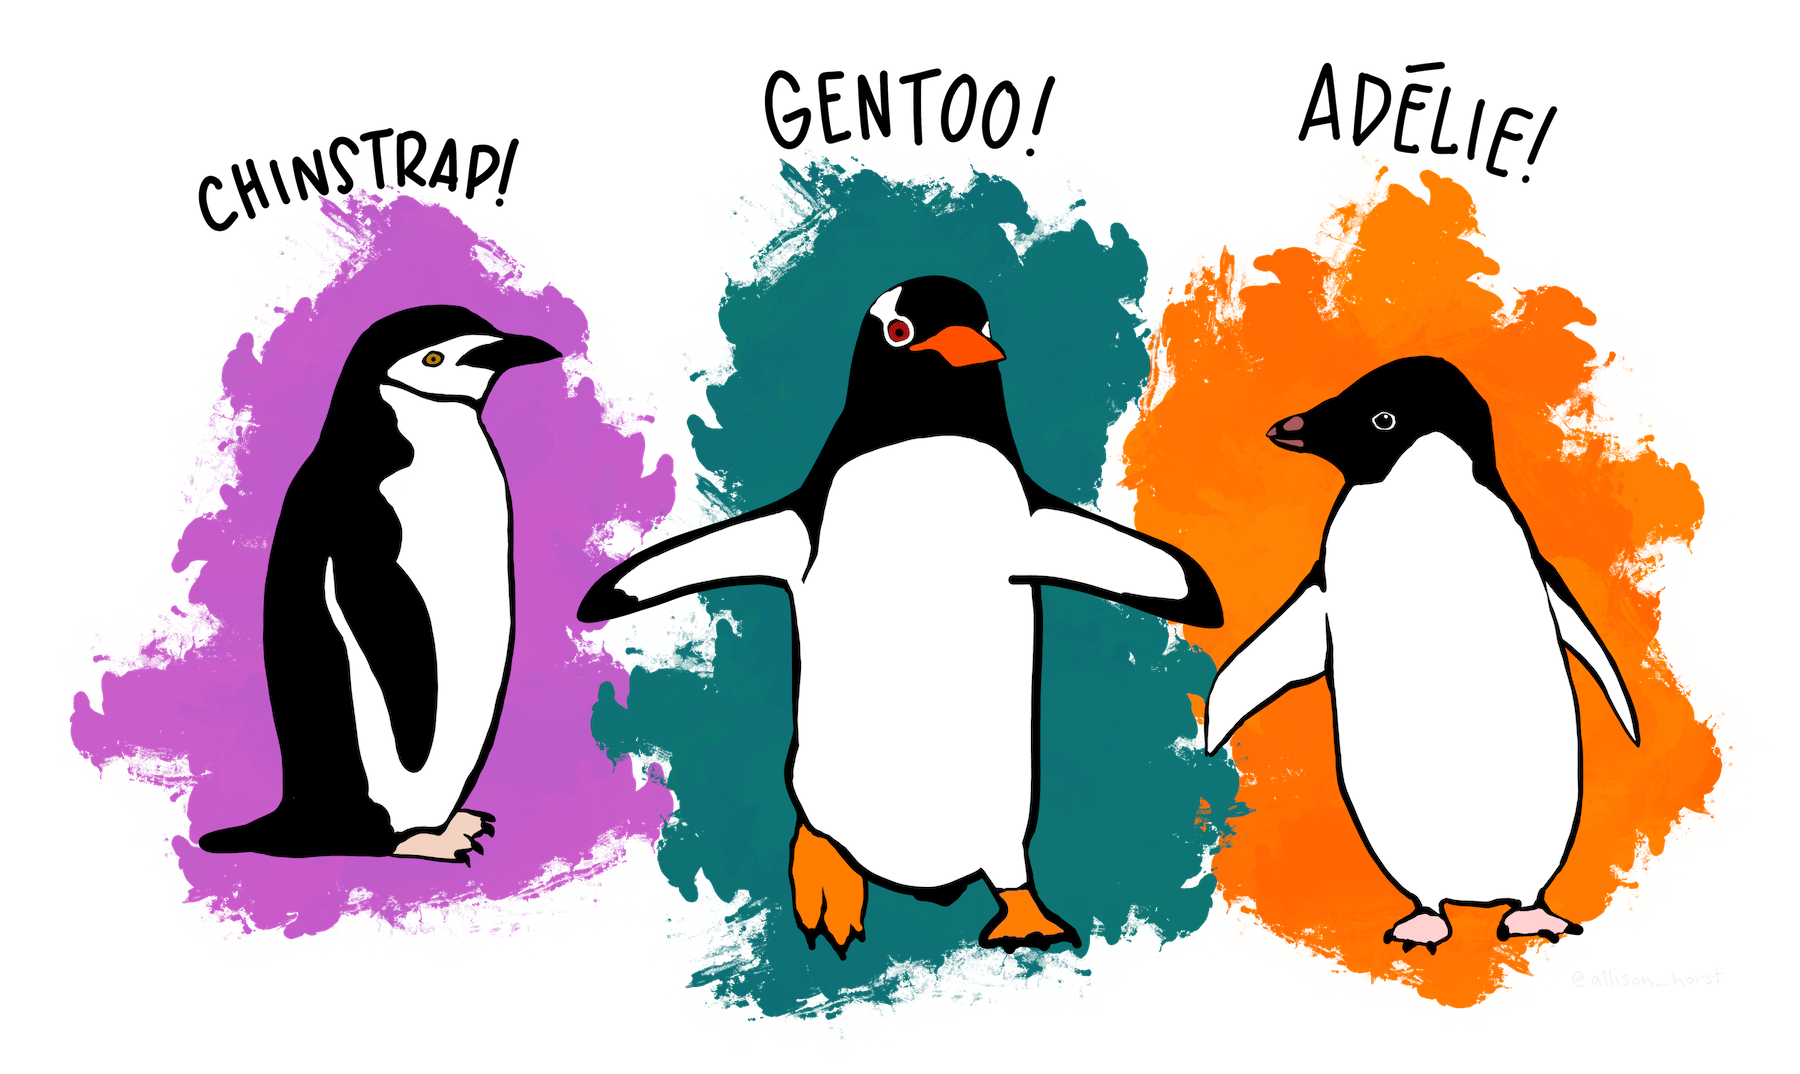
\includegraphics[width=0.75\linewidth]{./images/lter_penguins} 

}

\caption{Meet the Palmer penguins (artwork by Allison Horst)}\label{fig:unnamed-chunk-102}
\end{figure}

Why use this data set? Apart from the fact that everyone likes penguins, obviously, these data are sufficiently complex to demonstrate everything we want to do, while remaining easily understandable. Here is the full data set shown as a table:

\emph{N.B. --- the data will only show up in the HTML version of the book.}

This shows the first ten rows along with the first few columns. The \emph{Previous / Next} links at the bottom right can be used to navigate the rows; the arrows in the top header row are used to view the different columns. Below each column name you can also see three-letter abbreviations like \texttt{\textless{}dbl\textgreater{}}, \texttt{\textless{}int\textgreater{}} and \texttt{\textless{}chr\textgreater{}}. These are telling us that each column is a vector of some kind:

\begin{itemize}
\item
  \texttt{\textless{}dbl\textgreater{}} = a numeric `double' vector (real numbers, i.e.~with decimals)
\item
  \texttt{\textless{}int\textgreater{}} = a numeric integer vector (integer numbers)
\item
  \texttt{\textless{}chr\textgreater{}} = character vector.
\end{itemize}

So\ldots{} data frames are table-like objects with rows and columns. They can also be seen in even simpler terms---data frames are simply collections of vectors, where each one represents a different aspect of a multi-faceted data set.

We're going to be seeing a lot of this data set in the remaining chapters so we won't say anything more about it now.

\begin{infobox}{information}

\hypertarget{where-can-we-get-the-penguins-data}{%
\subsubsection*{Where can we get the penguins data?}\label{where-can-we-get-the-penguins-data}}
\addcontentsline{toc}{subsubsection}{Where can we get the penguins data?}

The Palmer penguins data were collected and made available by \href{https://www.uaf.edu/cfos/people/faculty/detail/kristen-gorman.php}{Dr.~Kristen Gorman} and the \href{https://pal.lternet.edu/}{Palmer Station}. The data set exists mostly to support people learning and teaching R. It isn't part of base R, though. We have to import it into R somehow. There are two options:

\begin{enumerate}
\def\labelenumi{\arabic{enumi}.}
\item
  The data are available in an R package called\ldots{} \href{https://allisonhorst.github.io/palmerpenguins/index.html}{palmerpenguins}. Like other packages, \textbf{palmerpenguins} can be installed from \href{https://cran.r-project.org/web/packages/palmerpenguins/index.html}{CRAN} using either \texttt{install.packages} or the usual RStudio point-and-click mechanism. Once installed, we can make it available by running \texttt{library(palmerpenguins)} in any R session. After that, just type the name of the data set and R will find it and use it. The version in \textbf{palmerpenguins} is called \texttt{penguins}, by the way.
\item
  We could get a copy of the data set and store it as a file on our hard drive, ideally using a standard data format. The most common and portable format for storing rectangular data is as a `Comma Separated Value' (CSV) text file. Once you have a copy of the data as a CSV file, it's just a matter of using a function like read\_csv from the readr package to import the data into R. This is explained in the \protect\hyperlink{project-scripts-data}{Managing projects, scripts and data files} appendix.
\end{enumerate}

\end{infobox}

\hypertarget{um-tibbles}{%
\section{Um\ldots{} tibbles?}\label{um-tibbles}}

To increase the scope of what the tidyverse can do, its makers created a special kind of data object known as a `tibble'. This is meant to sound like the word `table' pronounced by a New Zealander. We're not lying---the person who started the tidyverse is from New Zealand. Its name is a clue that a tibble is a table-like object, i.e.~a rectangular data structure similar to a data frame.

In fact, the easiest way to conceptualise a tibble is as a special data frame with a few extra whistles and bells. More often than not, it's not necessary to pay attention to whether we're working with an ordinary data frame or a tidyverse tibble---we can often treat them as though they are interchangeable.

That said, there are exceptions to this rule of thumb, and we do occasionally need to work out which one we're using. A simple way to do this is by printing the data object. Imagine that we've imported the Palmer penguins into R and stored it in a tibble called \texttt{penguins}. This is what that would look like if we printed it at the Console:

\begin{Shaded}
\begin{Highlighting}[]
\NormalTok{penguins}
\end{Highlighting}
\end{Shaded}

\begin{verbatim}
## # A tibble: 344 x 8
##    species island bill_length_mm bill_depth_mm flipper_length_~ body_mass_g
##    <chr>   <chr>           <dbl>         <dbl>            <int>       <int>
##  1 Adelie  Torge~           39.1          18.7              181        3750
##  2 Adelie  Torge~           39.5          17.4              186        3800
##  3 Adelie  Torge~           40.3          18                195        3250
##  4 Adelie  Torge~           NA            NA                 NA          NA
##  5 Adelie  Torge~           36.7          19.3              193        3450
##  6 Adelie  Torge~           39.3          20.6              190        3650
##  7 Adelie  Torge~           38.9          17.8              181        3625
##  8 Adelie  Torge~           39.2          19.6              195        4675
##  9 Adelie  Torge~           34.1          18.1              193        3475
## 10 Adelie  Torge~           42            20.2              190        4250
## # ... with 334 more rows, and 2 more variables: sex <chr>, year <int>
\end{verbatim}

The formatting applied to the output is telling us \texttt{penguins} is a tibble rather than an ordinary data frame (we only called it a data frame earlier because we had not introduced the concept of a tibble yet). There are a couple of clues about this in that printout. The very obvious one is the first line: \texttt{\#\ A\ tibble:\ 344\ x\ 8}. The printed output states \texttt{penguins} is a tibble! The output is also truncated---only the first ten lines were printed, and any columns that won't fit on one row are summarised at the bottom (i.e.~\texttt{sex} and \texttt{year}).

\hypertarget{missing-values}{%
\section{Missing values}\label{missing-values}}

Take a close look at the values of the body mass data (\texttt{body\_mass\_g}) in \texttt{penguins} (we're using \texttt{\$} to extract the whole column):

\begin{Shaded}
\begin{Highlighting}[]
\NormalTok{penguins}\SpecialCharTok{$}\NormalTok{body\_mass\_g}
\end{Highlighting}
\end{Shaded}

\begin{verbatim}
##   [1] 3750 3800 3250   NA 3450 3650 3625 4675 3475 4250 3300 3700 3200 3800 4400
##  [16] 3700 3450 4500 3325 4200 3400 3600 3800 3950 3800 3800 3550 3200 3150 3950
##  [31] 3250 3900 3300 3900 3325 4150 3950 3550 3300 4650 3150 3900 3100 4400 3000
##  [46] 4600 3425 2975 3450 4150 3500 4300 3450 4050 2900 3700 3550 3800 2850 3750
##  [61] 3150 4400 3600 4050 2850 3950 3350 4100 3050 4450 3600 3900 3550 4150 3700
##  [76] 4250 3700 3900 3550 4000 3200 4700 3800 4200 3350 3550 3800 3500 3950 3600
##  [91] 3550 4300 3400 4450 3300 4300 3700 4350 2900 4100 3725 4725 3075 4250 2925
## [106] 3550 3750 3900 3175 4775 3825 4600 3200 4275 3900 4075 2900 3775 3350 3325
## [121] 3150 3500 3450 3875 3050 4000 3275 4300 3050 4000 3325 3500 3500 4475 3425
## [136] 3900 3175 3975 3400 4250 3400 3475 3050 3725 3000 3650 4250 3475 3450 3750
## [151] 3700 4000 4500 5700 4450 5700 5400 4550 4800 5200 4400 5150 4650 5550 4650
## [166] 5850 4200 5850 4150 6300 4800 5350 5700 5000 4400 5050 5000 5100 4100 5650
## [181] 4600 5550 5250 4700 5050 6050 5150 5400 4950 5250 4350 5350 3950 5700 4300
## [196] 4750 5550 4900 4200 5400 5100 5300 4850 5300 4400 5000 4900 5050 4300 5000
## [211] 4450 5550 4200 5300 4400 5650 4700 5700 4650 5800 4700 5550 4750 5000 5100
## [226] 5200 4700 5800 4600 6000 4750 5950 4625 5450 4725 5350 4750 5600 4600 5300
## [241] 4875 5550 4950 5400 4750 5650 4850 5200 4925 4875 4625 5250 4850 5600 4975
## [256] 5500 4725 5500 4700 5500 4575 5500 5000 5950 4650 5500 4375 5850 4875 6000
## [271] 4925   NA 4850 5750 5200 5400 3500 3900 3650 3525 3725 3950 3250 3750 4150
## [286] 3700 3800 3775 3700 4050 3575 4050 3300 3700 3450 4400 3600 3400 2900 3800
## [301] 3300 4150 3400 3800 3700 4550 3200 4300 3350 4100 3600 3900 3850 4800 2700
## [316] 4500 3950 3650 3550 3500 3675 4450 3400 4300 3250 3675 3325 3950 3600 4050
## [331] 3350 3450 3250 4050 3800 3525 3950 3650 3650 4000 3400 3775 4100 3775
\end{verbatim}

The body mass information lives in a numeric (integer) vector, but not every element in that vector is a number. Two values are \texttt{NA}. That stands for `Not Available'---the \texttt{NA}'s job is to label cases where a value is missing or unknown. If you scroll around the table view of \texttt{penguins} above you'll find \texttt{NA}'s in several of the columns.

Missing data crop up all the time. They are just one of those facts of life---maybe the recording machine broke one afternoon, perhaps one of our organisms was infected by a pathogen, or maybe a cow ate one of our experimental plots. One of the nice things about R is that it knows how to represent missing data. It does this using the \texttt{NA} symbol.

You need to be aware of missing values when they are present. Why? Because the behaviour of many functions is affected by the presence of \texttt{NA}s. Things get confusing if we don't understand that behaviour. We will see some examples of this in the next few chapters.

\hypertarget{why-dplyr}{%
\section{\texorpdfstring{Introducing \textbf{dplyr}}{Introducing dplyr}}\label{why-dplyr}}

The \textbf{dplyr} package has been carefully designed to make it easy to manipulate `rectangular data', such as data frames. \textbf{dplyr} is very consistent in the way its functions work. For example, the first argument of the main \textbf{dplyr} functions is always an object containing our data. This consistency makes it very easy to get to grips with each of the main \textbf{dplyr} functions---it's often possible to understand how one works by seeing one or two examples of its use.

Another reason for using \textbf{dplyr} is that it is orientated around a few core functions, each designed to do one thing well. These \textbf{dplyr} functions are sometimes referred to as its `verbs' to reflect the fact that they `do something' to data. For example:

\begin{itemize}
\tightlist
\item
  \texttt{select} is obtains a subset of variables,
\item
  \texttt{mutate} is constructs new variables,
\item
  \texttt{filter} is obtains a subset of rows,
\item
  \texttt{arrange} is reorders rows, and
\item
  \texttt{summarise} is calculates information about groups.
\end{itemize}

Notice that the names are chosen to reflect what each verb/function does to the input data. We'll cover each of these verbs in detail in later chapters, as well as a few additional ones, such as \texttt{rename} and \texttt{group\_by}.

Apart from being easy to use, \textbf{dplyr} is also fast. This doesn't matter for small data sets but can be important when working with data sets with hundreds of thousands of rows. The \textbf{dplyr} package also allows us to work with data stored in different ways, for example, by interacting directly with several database systems. We're going to focus on using it with data frames and tibbles. But remember---once you know how to use \textbf{dplyr} with data frames its easy to use it for work with other kinds of data sources.

\begin{infobox}{information}

\hypertarget{a-dplyr-cheat-sheet}{%
\subsubsection*{\texorpdfstring{A \textbf{dplyr} cheat sheet}{A dplyr cheat sheet}}\label{a-dplyr-cheat-sheet}}
\addcontentsline{toc}{subsubsection}{A \textbf{dplyr} cheat sheet}

The developers of RStudio have produced a very usable \href{http://www.rstudio.com/resources/cheatsheets/}{cheat sheat} that summarises the main data wrangling tools provided by \textbf{dplyr}.

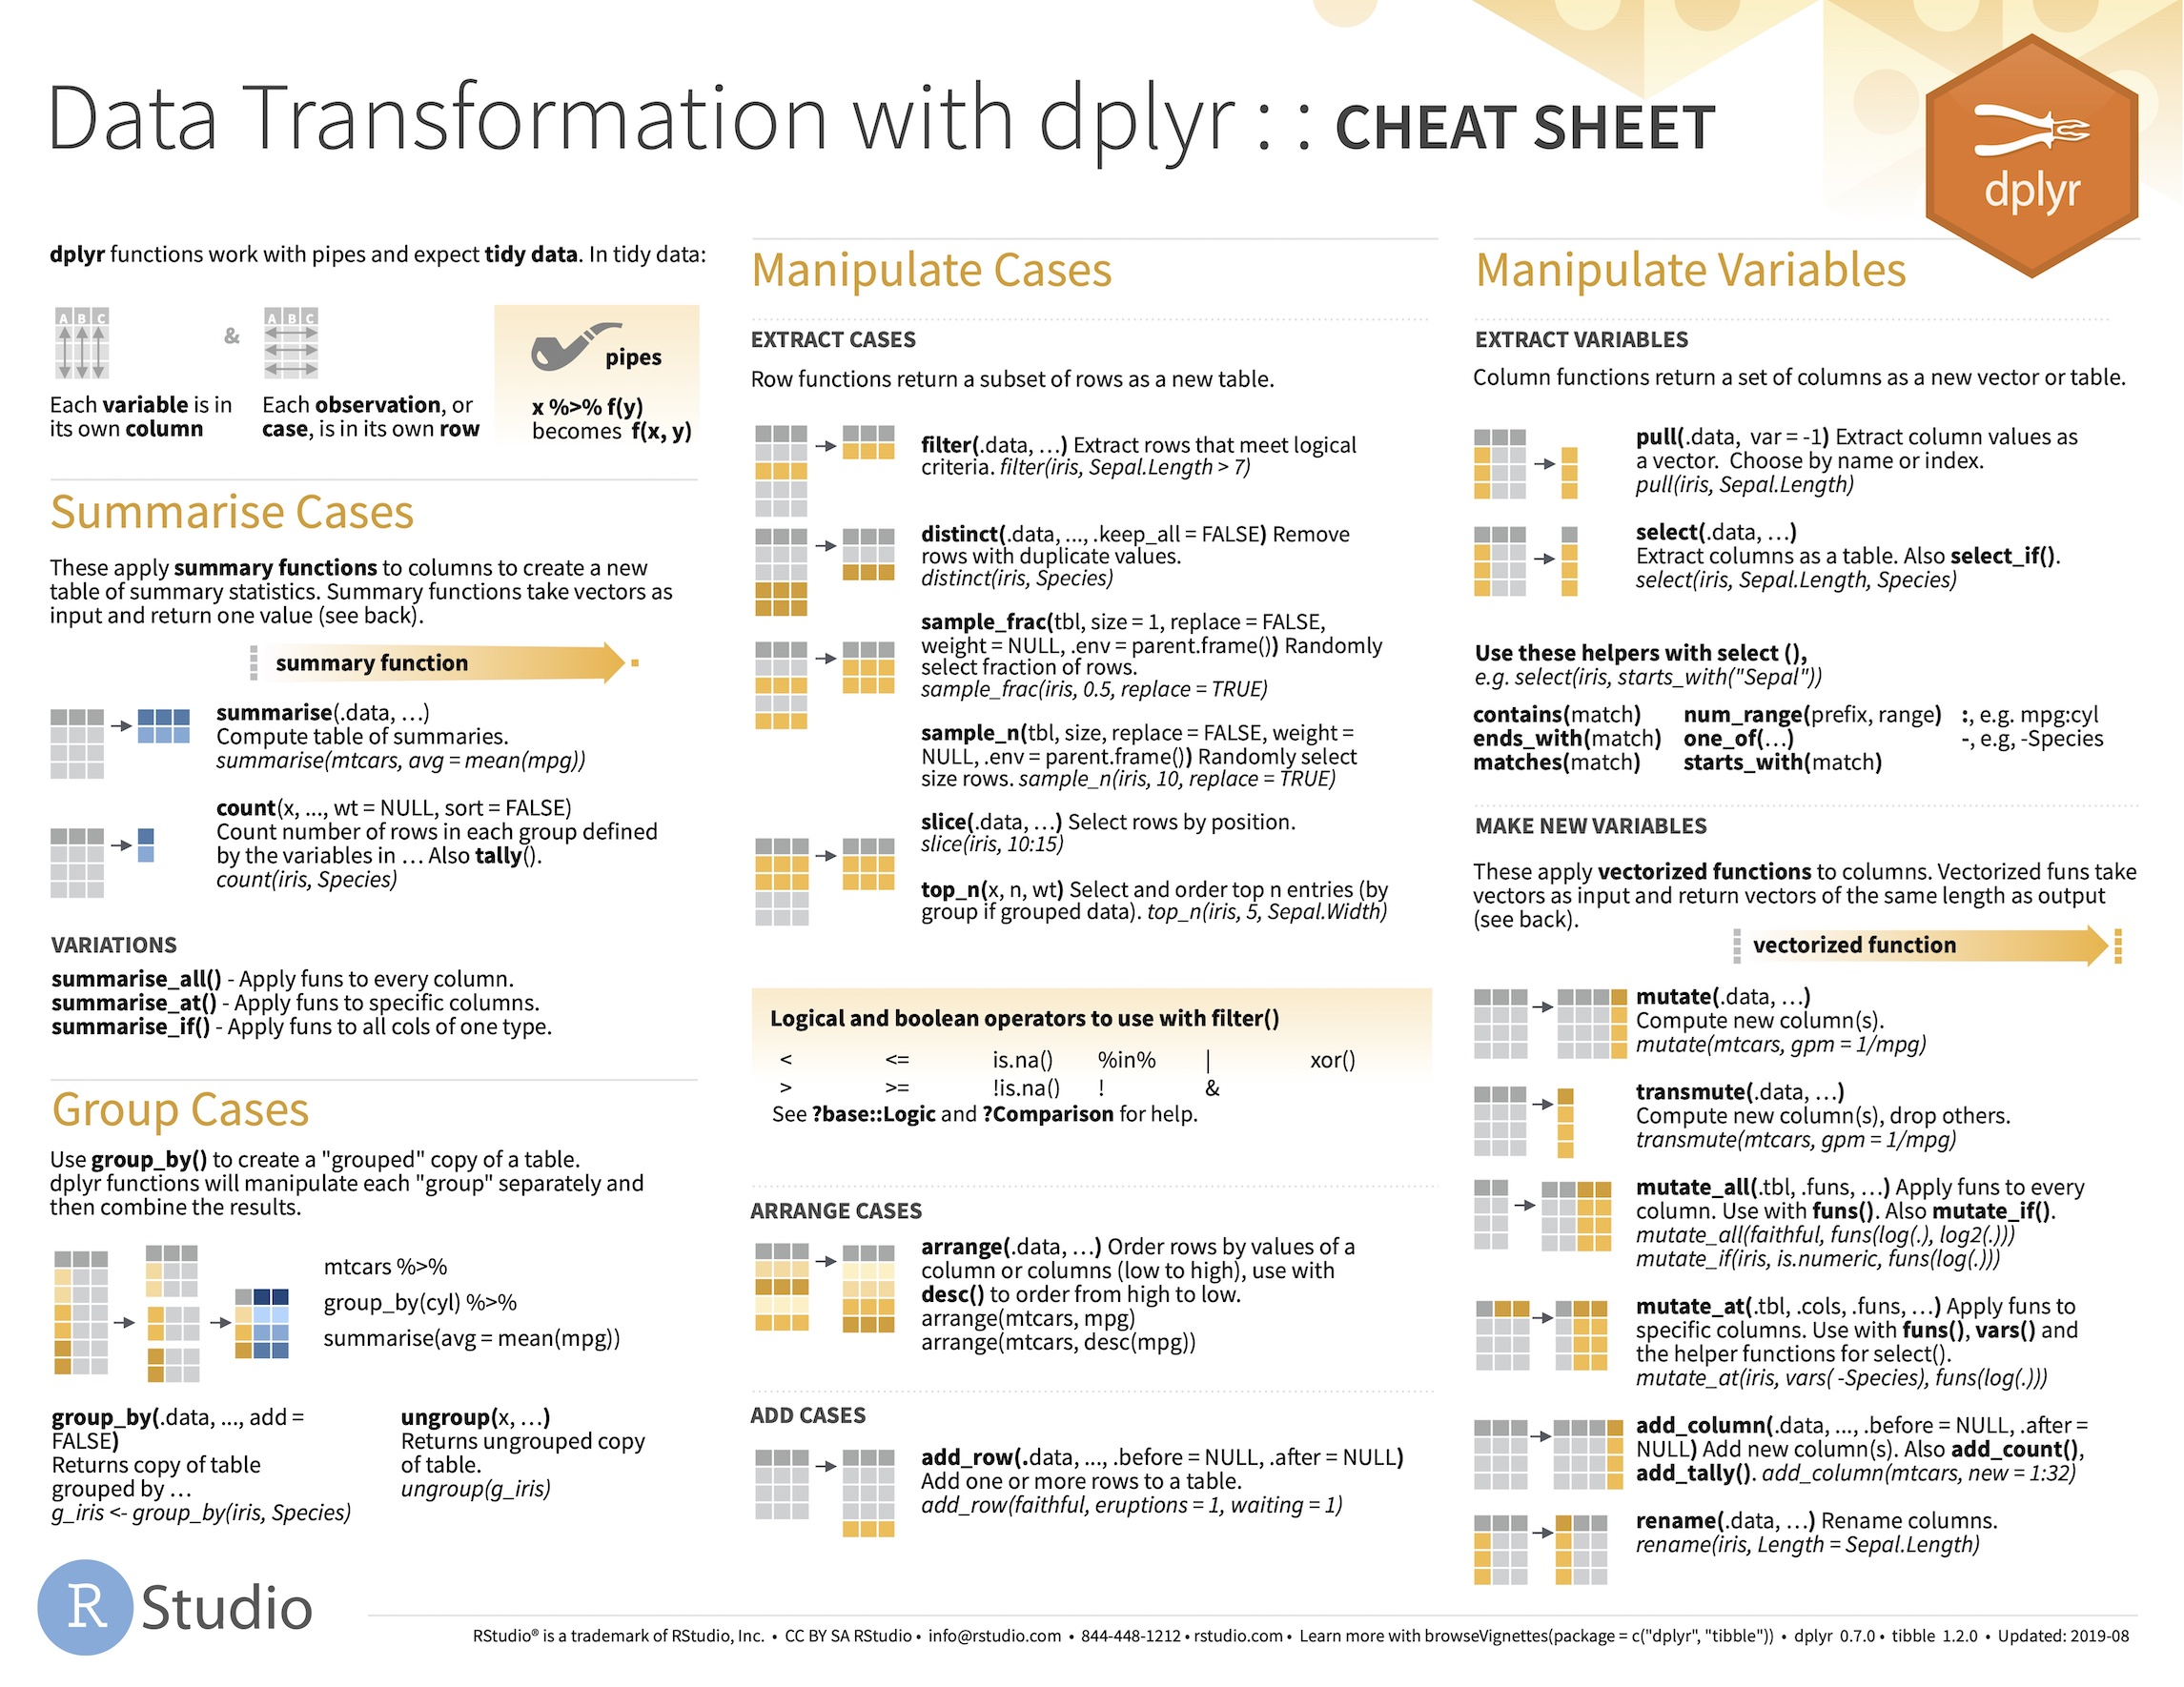
\includegraphics{images/data-transformation.jpg}

Our advice is to download this, print out a copy, and refer to it often as you start working with \textbf{dplyr}.

\end{infobox}

\hypertarget{more-dplyr}{%
\subsection{\texorpdfstring{A first look at \textbf{dplyr}}{A first look at dplyr}}\label{more-dplyr}}

We'll draw this chapter to a close by taking a preliminary look at the \textbf{dplyr} package. The package is not part of the base R installation, so we have to have installed it first. Remember, once installed, there is no need to install the package every time we need to use it. We do have to use \texttt{library} to load and attach the package every time we want to use it:

\begin{Shaded}
\begin{Highlighting}[]
\FunctionTok{library}\NormalTok{(}\StringTok{"dplyr"}\NormalTok{)}
\end{Highlighting}
\end{Shaded}

Let's look at one handy \textbf{dplyr} function now. Sometimes we just need a quick, compact summary of a data frame or tibble. This is the job of the \texttt{glimpse} function from \textbf{dplyr}:

\begin{Shaded}
\begin{Highlighting}[]
\FunctionTok{glimpse}\NormalTok{(penguins)}
\end{Highlighting}
\end{Shaded}

\begin{verbatim}
## Rows: 344
## Columns: 8
## $ species           <chr> "Adelie", "Adelie", "Adelie", "Adelie", "Adelie",...
## $ island            <chr> "Torgersen", "Torgersen", "Torgersen", "Torgersen...
## $ bill_length_mm    <dbl> 39.1, 39.5, 40.3, NA, 36.7, 39.3, 38.9, 39.2, 34....
## $ bill_depth_mm     <dbl> 18.7, 17.4, 18.0, NA, 19.3, 20.6, 17.8, 19.6, 18....
## $ flipper_length_mm <int> 181, 186, 195, NA, 193, 190, 181, 195, 193, 190, ...
## $ body_mass_g       <int> 3750, 3800, 3250, NA, 3450, 3650, 3625, 4675, 347...
## $ sex               <chr> "male", "female", "female", NA, "female", "male",...
## $ year              <int> 2007, 2007, 2007, 2007, 2007, 2007, 2007, 2007, 2...
\end{verbatim}

The function takes one argument: the name of a data frame or tibble. It then tells us how many rows it has, how many columns there are, what these columns are called, and what type of data is associated with them. This function is useful when we need a quick overview of what's inside our data set. Some advice---use this function on any new data set before trying to do anything with it.

\hypertarget{dplyr-pseudocode}{%
\subsection{\texorpdfstring{\textbf{dplyr} pseudocode}{dplyr pseudocode}}\label{dplyr-pseudocode}}

We'll wrap-up this chapter with a quick mention of `pseudocode'. Pseudocode uses structural conventions of normal R code but is intended for us (humans) to read rather than the computer. We use it summarise how \textbf{dplyr} functions work. Here's an example you will encounter in the next chapter:

\begin{Shaded}
\begin{Highlighting}[]
\FunctionTok{select}\NormalTok{(}\SpecialCharTok{\textless{}}\NormalTok{data}\SpecialCharTok{\textgreater{}}\NormalTok{, }\SpecialCharTok{\textless{}}\NormalTok{variable}\DecValTok{{-}1}\SpecialCharTok{\textgreater{}}\NormalTok{, }\SpecialCharTok{\textless{}}\NormalTok{variable}\DecValTok{{-}2}\SpecialCharTok{\textgreater{}}\NormalTok{, ...)}
\end{Highlighting}
\end{Shaded}

\textbf{This is not an example we can run.} It is pseudocode that serves as a template for using the \textbf{dplyr} \texttt{select} function. The words surrounded by `angle brackets' (\texttt{\textless{}\ \textgreater{}}) are placeholders. If we want to turn this pseudocode into real R code we have to \textbf{replace those placeholders}. For example, \texttt{\textless{}data\textgreater{}} is a placeholder for the name of a data set. We would replace that with the word \texttt{penguins} if we want to use select on our example data set (we'd also have to do something with the other placeholders (e.g.~\texttt{\textless{}variable-1\textgreater{}})---we'll get to that later).

That's enough about pseudocode and \textbf{dplyr} templates. We'll see plenty of these in the next few chapters.

\hypertarget{working-with-variables}{%
\chapter{Working with variables}\label{working-with-variables}}

\hypertarget{introduction-3}{%
\section{Introduction}\label{introduction-3}}

This chapter will explore the \textbf{dplyr} \texttt{select} and \texttt{mutate} verbs, and the closely related \texttt{rename} and \texttt{transmute} verbs. We consider these functions together because they operate on the variables (i.e.~the columns) of a data frame or tibble:

\begin{itemize}
\tightlist
\item
  The \texttt{select} function selects a subset of variables to retain and (optionally) renames them in the process.
\item
  The \texttt{mutate} function creates new variables from pre-existing ones and retains the original variables.
\item
  The \texttt{rename} function renames one or more variables while keeping the remaining variable names unchanged.
\item
  The \texttt{transmute} function creates new variables from pre-existing ones and drops the original variables.
\end{itemize}

\hypertarget{getting-ready}{%
\subsection{Getting ready}\label{getting-ready}}

Obviously, we need to have first installed \textbf{dplyr} package to use it. Assuming that's been done, we need to load and attach the package in the current session:

\begin{Shaded}
\begin{Highlighting}[]
\FunctionTok{library}\NormalTok{(}\StringTok{"dplyr"}\NormalTok{)}
\end{Highlighting}
\end{Shaded}

We will use the Palmer penguins data to illustrate the ideas in this chapter. Remember---the \protect\hyperlink{penguins-data-overview}{previous chapter} described this data set and explained where to find it. The examples below assume it was read into R as a tibble with the name \texttt{penguins}.

\hypertarget{subset-variables-with-select}{%
\section{\texorpdfstring{Subset variables with \texttt{select}}{Subset variables with select}}\label{subset-variables-with-select}}

We use \texttt{select} to \textbf{select variables} from a data frame or tibble. This is used when we have a data set with many variables but only need to work with a subset of these. Basic usage of \texttt{select} looks like this:

\begin{Shaded}
\begin{Highlighting}[]
\FunctionTok{select}\NormalTok{(}\SpecialCharTok{\textless{}}\NormalTok{data}\SpecialCharTok{\textgreater{}}\NormalTok{, }\SpecialCharTok{\textless{}}\NormalTok{variable}\DecValTok{{-}1}\SpecialCharTok{\textgreater{}}\NormalTok{, }\SpecialCharTok{\textless{}}\NormalTok{variable}\DecValTok{{-}2}\SpecialCharTok{\textgreater{}}\NormalTok{, ...)}
\end{Highlighting}
\end{Shaded}

Remember---this is not an example we can run. This is a pseudocode designed to provide a generic description of how we use \texttt{select}. Let's look at the arguments of select:

\begin{itemize}
\tightlist
\item
  The first argument, \texttt{\textless{}data\textgreater{}}, must be the name of the object containing our data (usually a data frame or tibble). This is not optional---\textbf{dplyr} functions only exist to manipulate data.
\item
  We then include a series of one or more additional arguments, where each one is the name of a variable in \texttt{\textless{}data\textgreater{}}. We've expressed this as \texttt{\textless{}variable-1\textgreater{},\ \textless{}variable-2\textgreater{},\ ...}, where \texttt{\textless{}variable-1\textgreater{}} and \texttt{\textless{}variable-2\textgreater{}} are names of the first two variables. The \texttt{...} is acting as a placeholder for the remaining variables. There could be any number of these.
\end{itemize}

It's easiest to understand how a function like \texttt{select} works by seeing it in action. We select the \texttt{species}, \texttt{bill\_length\_mm} and \texttt{bill\_depth\_mm} variables from \texttt{penguins} like this:

\begin{Shaded}
\begin{Highlighting}[]
\FunctionTok{select}\NormalTok{(penguins, species, bill\_length\_mm, bill\_depth\_mm)}
\end{Highlighting}
\end{Shaded}

\begin{verbatim}
## # A tibble: 344 x 3
##    species bill_length_mm bill_depth_mm
##    <chr>            <dbl>         <dbl>
##  1 Adelie            39.1          18.7
##  2 Adelie            39.5          17.4
##  3 Adelie            40.3          18  
##  4 Adelie            NA            NA  
##  5 Adelie            36.7          19.3
##  6 Adelie            39.3          20.6
##  7 Adelie            38.9          17.8
##  8 Adelie            39.2          19.6
##  9 Adelie            34.1          18.1
## 10 Adelie            42            20.2
## # ... with 334 more rows
\end{verbatim}

Hopefully, nothing about this example is too surprising. However, there are a few subtleties buried in that example:

\begin{itemize}
\tightlist
\item
  The \texttt{select} function is designed to work in a non-standard way which means variable names should \textbf{not} be surrounded by quotes. The one exception is when a name has a space in it. Under those circumstances, it has to be quoted with backticks, e.g.~\texttt{\textasciigrave{}variable\ 1\textasciigrave{}}.
\item
  The \texttt{select} function does not have `side effects'. This means is that it does not change the original \texttt{penguins} object. We printed the result produced by \texttt{select} to the Console, so we can't access the modified data set. If we need to use the result, we have to assign it a name using \texttt{\textless{}-}.
\item
  The order of variables (i.e.~the column order) in the resulting object is the same as the order in which they were supplied to the argument list. This means we can reorder variables at the same time as selecting them if we need to.
\item
  The \texttt{select} function will return the same kind of data object we give it to work on. It returns a data frame if our data was in a data frame and a tibble if it was a tibble. In this example, R prints a tibble because \texttt{penguins} was a tibble.
\end{itemize}

That second point is important---we have to remember to assign the result a name using \texttt{\textless{}-} if we want to keep it and use it later. For example, we might call the result of that last example \texttt{penguins\_bill}:

\begin{Shaded}
\begin{Highlighting}[]
\NormalTok{penguins\_bill }\OtherTok{\textless{}{-}} \FunctionTok{select}\NormalTok{(penguins, species, bill\_length\_mm, bill\_depth\_mm)}
\end{Highlighting}
\end{Shaded}

Now that we've named the new data set created by \texttt{select} we can refer to it by that name whenever we need it:

\begin{Shaded}
\begin{Highlighting}[]
\NormalTok{penguins\_bill}
\end{Highlighting}
\end{Shaded}

\begin{verbatim}
## # A tibble: 344 x 3
##    species bill_length_mm bill_depth_mm
##    <chr>            <dbl>         <dbl>
##  1 Adelie            39.1          18.7
##  2 Adelie            39.5          17.4
##  3 Adelie            40.3          18  
##  4 Adelie            NA            NA  
##  5 Adelie            36.7          19.3
##  6 Adelie            39.3          20.6
##  7 Adelie            38.9          17.8
##  8 Adelie            39.2          19.6
##  9 Adelie            34.1          18.1
## 10 Adelie            42            20.2
## # ... with 334 more rows
\end{verbatim}

Remember---the original \texttt{penguins} data is completely unchanged:

\begin{Shaded}
\begin{Highlighting}[]
\NormalTok{penguins}
\end{Highlighting}
\end{Shaded}

\begin{verbatim}
## # A tibble: 344 x 8
##    species island bill_length_mm bill_depth_mm flipper_length_~ body_mass_g
##    <chr>   <chr>           <dbl>         <dbl>            <int>       <int>
##  1 Adelie  Torge~           39.1          18.7              181        3750
##  2 Adelie  Torge~           39.5          17.4              186        3800
##  3 Adelie  Torge~           40.3          18                195        3250
##  4 Adelie  Torge~           NA            NA                 NA          NA
##  5 Adelie  Torge~           36.7          19.3              193        3450
##  6 Adelie  Torge~           39.3          20.6              190        3650
##  7 Adelie  Torge~           38.9          17.8              181        3625
##  8 Adelie  Torge~           39.2          19.6              195        4675
##  9 Adelie  Torge~           34.1          18.1              193        3475
## 10 Adelie  Torge~           42            20.2              190        4250
## # ... with 334 more rows, and 2 more variables: sex <chr>, year <int>
\end{verbatim}

\hypertarget{alternative-ways-to-identify-variables-with-select}{%
\subsection{\texorpdfstring{Alternative ways to identify variables with \texttt{select}}{Alternative ways to identify variables with select}}\label{alternative-ways-to-identify-variables-with-select}}

It's sometimes more convenient to use \texttt{select} to subset variables by specifying those we do \textbf{not} need, rather than specifying of the ones to keep. We can use the \texttt{!} operator to indicate that certain variables should be dropped. For example, to get rid of the \texttt{bill\_depth\_mm} and \texttt{bill\_length\_mm} columns, we could use:

\begin{Shaded}
\begin{Highlighting}[]
\FunctionTok{select}\NormalTok{(penguins, }\SpecialCharTok{!}\NormalTok{bill\_depth\_mm, }\SpecialCharTok{!}\NormalTok{bill\_length\_mm)}
\end{Highlighting}
\end{Shaded}

\begin{verbatim}
## # A tibble: 344 x 8
##    species island bill_length_mm flipper_length_~ body_mass_g sex    year
##    <chr>   <chr>           <dbl>            <int>       <int> <chr> <int>
##  1 Adelie  Torge~           39.1              181        3750 male   2007
##  2 Adelie  Torge~           39.5              186        3800 fema~  2007
##  3 Adelie  Torge~           40.3              195        3250 fema~  2007
##  4 Adelie  Torge~           NA                 NA          NA <NA>   2007
##  5 Adelie  Torge~           36.7              193        3450 fema~  2007
##  6 Adelie  Torge~           39.3              190        3650 male   2007
##  7 Adelie  Torge~           38.9              181        3625 fema~  2007
##  8 Adelie  Torge~           39.2              195        4675 male   2007
##  9 Adelie  Torge~           34.1              193        3475 <NA>   2007
## 10 Adelie  Torge~           42                190        4250 <NA>   2007
## # ... with 334 more rows, and 1 more variable: bill_depth_mm <dbl>
\end{verbatim}

This returns a tibble with all the other variables: \texttt{species}, \texttt{island}, \texttt{flipper\_length\_mm}, \texttt{body\_mass\_g}, \texttt{sex} and \texttt{year}.

The \texttt{select} function can also be used to grab (or drop) a set of variables that occur in a sequence next to one another. We specify a series of adjacent variables using the \texttt{:} operator. We use this with two variable names, one on the left-hand side and one on the right. When we use \texttt{:} like this, \texttt{select} will subset both those two variables along with any others that fall in between them.

For example, if we want only the morphometric variables (\texttt{bill\_length\_mm}, \texttt{bill\_depth\_mm}, \texttt{flipper\_length\_mm} and \texttt{body\_mass\_g}) we could use:

\begin{Shaded}
\begin{Highlighting}[]
\FunctionTok{select}\NormalTok{(penguins, bill\_length\_mm}\SpecialCharTok{:}\NormalTok{body\_mass\_g)}
\end{Highlighting}
\end{Shaded}

\begin{verbatim}
## # A tibble: 344 x 4
##    bill_length_mm bill_depth_mm flipper_length_mm body_mass_g
##             <dbl>         <dbl>             <int>       <int>
##  1           39.1          18.7               181        3750
##  2           39.5          17.4               186        3800
##  3           40.3          18                 195        3250
##  4           NA            NA                  NA          NA
##  5           36.7          19.3               193        3450
##  6           39.3          20.6               190        3650
##  7           38.9          17.8               181        3625
##  8           39.2          19.6               195        4675
##  9           34.1          18.1               193        3475
## 10           42            20.2               190        4250
## # ... with 334 more rows
\end{verbatim}

The \texttt{:} operator can also be combined with \texttt{!} if we need to drop a series of variables according to their position in a data frame or tibble. For example, we can use this trick to get the complement of the previous example, i.e.~throw away the morphometric variables:

\begin{Shaded}
\begin{Highlighting}[]
\FunctionTok{select}\NormalTok{(penguins, }\SpecialCharTok{!}\NormalTok{bill\_length\_mm}\SpecialCharTok{:}\NormalTok{body\_mass\_g)}
\end{Highlighting}
\end{Shaded}

\begin{verbatim}
## # A tibble: 344 x 4
##    species island    sex     year
##    <chr>   <chr>     <chr>  <int>
##  1 Adelie  Torgersen male    2007
##  2 Adelie  Torgersen female  2007
##  3 Adelie  Torgersen female  2007
##  4 Adelie  Torgersen <NA>    2007
##  5 Adelie  Torgersen female  2007
##  6 Adelie  Torgersen male    2007
##  7 Adelie  Torgersen female  2007
##  8 Adelie  Torgersen male    2007
##  9 Adelie  Torgersen <NA>    2007
## 10 Adelie  Torgersen <NA>    2007
## # ... with 334 more rows
\end{verbatim}

\hypertarget{renaming-variables-with-select-and-rename}{%
\subsection{\texorpdfstring{Renaming variables with \texttt{select} and \texttt{rename}}{Renaming variables with select and rename}}\label{renaming-variables-with-select-and-rename}}

The \texttt{select} function can also rename variables at the same time as selecting them. To do this, we name the arguments using the \texttt{name\ =\ value} construct, where the name of the selected variable is placed on the right-hand side (\texttt{value}), and the new name goes on the left-hand side (\texttt{name}).

For example, to select the\texttt{species}, \texttt{bill\_length\_mm} and \texttt{bill\_depth\_mm} variables from \texttt{penguins}, and in the process, rename \texttt{bill\_length\_mm} and \texttt{bill\_depth\_mm} to \texttt{BillLength} and \texttt{BillDepth}, use:

\begin{Shaded}
\begin{Highlighting}[]
\FunctionTok{select}\NormalTok{(penguins, species, }\AttributeTok{BillLength =}\NormalTok{ bill\_length\_mm, }\AttributeTok{BillDepth =}\NormalTok{ bill\_depth\_mm)}
\end{Highlighting}
\end{Shaded}

\begin{verbatim}
## # A tibble: 344 x 3
##    species BillLength BillDepth
##    <chr>        <dbl>     <dbl>
##  1 Adelie        39.1      18.7
##  2 Adelie        39.5      17.4
##  3 Adelie        40.3      18  
##  4 Adelie        NA        NA  
##  5 Adelie        36.7      19.3
##  6 Adelie        39.3      20.6
##  7 Adelie        38.9      17.8
##  8 Adelie        39.2      19.6
##  9 Adelie        34.1      18.1
## 10 Adelie        42        20.2
## # ... with 334 more rows
\end{verbatim}

Renaming the variables is a common task. What should we do if the only thing we want to achieve is to rename variables, rather than rename \emph{and} select them? \textbf{dplyr} provides an additional function called \texttt{rename} for exactly this purpose. This function renames some variables while retaining all others. It works like \texttt{select}. For example, to rename \texttt{bill\_length\_mm} and \texttt{bill\_depth\_mm} to \texttt{BillLength} and \texttt{BillDepth} but keep all the variables, use:

\begin{Shaded}
\begin{Highlighting}[]
\FunctionTok{rename}\NormalTok{(penguins, }\AttributeTok{BillLength =}\NormalTok{ bill\_length\_mm, }\AttributeTok{BillDepth =}\NormalTok{ bill\_depth\_mm)}
\end{Highlighting}
\end{Shaded}

\begin{verbatim}
## # A tibble: 344 x 8
##    species island  BillLength BillDepth flipper_length_~ body_mass_g sex    year
##    <chr>   <chr>        <dbl>     <dbl>            <int>       <int> <chr> <int>
##  1 Adelie  Torger~       39.1      18.7              181        3750 male   2007
##  2 Adelie  Torger~       39.5      17.4              186        3800 fema~  2007
##  3 Adelie  Torger~       40.3      18                195        3250 fema~  2007
##  4 Adelie  Torger~       NA        NA                 NA          NA <NA>   2007
##  5 Adelie  Torger~       36.7      19.3              193        3450 fema~  2007
##  6 Adelie  Torger~       39.3      20.6              190        3650 male   2007
##  7 Adelie  Torger~       38.9      17.8              181        3625 fema~  2007
##  8 Adelie  Torger~       39.2      19.6              195        4675 male   2007
##  9 Adelie  Torger~       34.1      18.1              193        3475 <NA>   2007
## 10 Adelie  Torger~       42        20.2              190        4250 <NA>   2007
## # ... with 334 more rows
\end{verbatim}

Notice \texttt{rename} also preserves the order of the variables found in the original data.

\hypertarget{creating-variables-with-mutate}{%
\section{\texorpdfstring{Creating variables with \texttt{mutate}}{Creating variables with mutate}}\label{creating-variables-with-mutate}}

We use \texttt{mutate} to \textbf{add new variables} to a data frame or tibble. This is useful if we need to construct one or more derived variables to support an analysis. Basic usage of \texttt{mutate} looks like this:

\begin{Shaded}
\begin{Highlighting}[]
\FunctionTok{mutate}\NormalTok{(}\SpecialCharTok{\textless{}}\NormalTok{data}\SpecialCharTok{\textgreater{}}\NormalTok{, }\SpecialCharTok{\textless{}}\NormalTok{expression}\DecValTok{{-}1}\SpecialCharTok{\textgreater{}}\NormalTok{, }\SpecialCharTok{\textless{}}\NormalTok{expression}\DecValTok{{-}2}\SpecialCharTok{\textgreater{}}\NormalTok{, ...)}
\end{Highlighting}
\end{Shaded}

Again, this is not an example we can run---it's pseudocode highlighting how to use \texttt{mutate} in abstract terms.

The first argument, \texttt{\textless{}data\textgreater{}}, must be the name of the object containing our data. We then include a series of one or more additional arguments, where each of these is a valid R expression involving one or more variables in \texttt{\textless{}data\textgreater{}}. We've have expressed these as \texttt{\textless{}expression-1\textgreater{},\ \textless{}expression-2\textgreater{}}, where \texttt{\textless{}expression-1\textgreater{}} and \texttt{\textless{}expression-2\textgreater{}} represent the first two expressions, and the \texttt{...} is acting as a placeholder for the remaining expressions. These can be any valid R code that refers to variables in \texttt{\textless{}data\textgreater{}}. This is often a simple calculation (e.g.~involving arithmetic), but it can be arbitrarily complex.

To see \texttt{mutate} in action, let's construct a new version of \texttt{penguins} that contains one extra variable---body mass measured in kilograms:

\begin{Shaded}
\begin{Highlighting}[]
\FunctionTok{mutate}\NormalTok{(penguins, body\_mass\_g }\SpecialCharTok{/} \DecValTok{1000}\NormalTok{)}
\end{Highlighting}
\end{Shaded}

\begin{verbatim}
## # A tibble: 344 x 9
##    species island bill_length_mm bill_depth_mm flipper_length_~ body_mass_g
##    <chr>   <chr>           <dbl>         <dbl>            <int>       <int>
##  1 Adelie  Torge~           39.1          18.7              181        3750
##  2 Adelie  Torge~           39.5          17.4              186        3800
##  3 Adelie  Torge~           40.3          18                195        3250
##  4 Adelie  Torge~           NA            NA                 NA          NA
##  5 Adelie  Torge~           36.7          19.3              193        3450
##  6 Adelie  Torge~           39.3          20.6              190        3650
##  7 Adelie  Torge~           38.9          17.8              181        3625
##  8 Adelie  Torge~           39.2          19.6              195        4675
##  9 Adelie  Torge~           34.1          18.1              193        3475
## 10 Adelie  Torge~           42            20.2              190        4250
## # ... with 334 more rows, and 3 more variables: sex <chr>, year <int>,
## #   `body_mass_g/1000` <dbl>
\end{verbatim}

This creates a copy of \texttt{penguins} with a new column called \texttt{body\_mass\_g/1000} (look at the bottom of the printed output). That is not a very good name but do not worry---we will improve on it in a moment. Most of the rules that apply to \texttt{select} also apply to \texttt{mutate}:

\begin{itemize}
\tightlist
\item
  Quotes must not be placed around an expression that performs a calculation.~ This makes sense because the expression is meant to be evaluated so that it ``does something''. It is not a value.
\item
  The \texttt{mutate} function does not have side effects, meaning it does not change the original \texttt{penguins} in any way. In the example, we printed the result produced by \texttt{mutate} rather than assigning it a name using \texttt{\textless{}-}, which means we have no way to access the result.
\item
  The \texttt{mutate} function returns the same kind of object as the one it is working on: a data frame if our data was originally in a data frame, a tibble if it was a tibble.
\end{itemize}

Creating a variable called something like \texttt{body\_mass\_g/1000} is not ideal because that is a difficult name to work with. Fortunately, the \texttt{mutate} function can name new variables at the same time as it creates them. We just name the arguments using \texttt{=}, placing the name on the left-hand side. Look at how to use this construct to name the new area variable \texttt{body\_mass\_kg}:

\begin{Shaded}
\begin{Highlighting}[]
\FunctionTok{mutate}\NormalTok{(penguins, }\AttributeTok{body\_mass\_kg =}\NormalTok{ body\_mass\_g }\SpecialCharTok{/} \DecValTok{1000}\NormalTok{)}
\end{Highlighting}
\end{Shaded}

\begin{verbatim}
## # A tibble: 344 x 9
##    species island bill_length_mm bill_depth_mm flipper_length_~ body_mass_g
##    <chr>   <chr>           <dbl>         <dbl>            <int>       <int>
##  1 Adelie  Torge~           39.1          18.7              181        3750
##  2 Adelie  Torge~           39.5          17.4              186        3800
##  3 Adelie  Torge~           40.3          18                195        3250
##  4 Adelie  Torge~           NA            NA                 NA          NA
##  5 Adelie  Torge~           36.7          19.3              193        3450
##  6 Adelie  Torge~           39.3          20.6              190        3650
##  7 Adelie  Torge~           38.9          17.8              181        3625
##  8 Adelie  Torge~           39.2          19.6              195        4675
##  9 Adelie  Torge~           34.1          18.1              193        3475
## 10 Adelie  Torge~           42            20.2              190        4250
## # ... with 334 more rows, and 3 more variables: sex <chr>, year <int>,
## #   body_mass_kg <dbl>
\end{verbatim}

We can create more than one variable by supplying \texttt{mutate} multiple (named) arguments:

\begin{Shaded}
\begin{Highlighting}[]
\FunctionTok{mutate}\NormalTok{(penguins, }
       \AttributeTok{bill\_size =}\NormalTok{ bill\_depth\_mm }\SpecialCharTok{*}\NormalTok{ bill\_length\_mm,}
       \AttributeTok{scaled\_bill\_size =}\NormalTok{ bill\_size }\SpecialCharTok{/}\NormalTok{ body\_mass\_g)}
\end{Highlighting}
\end{Shaded}

\begin{verbatim}
## # A tibble: 344 x 10
##    species island bill_length_mm bill_depth_mm flipper_length_~ body_mass_g
##    <chr>   <chr>           <dbl>         <dbl>            <int>       <int>
##  1 Adelie  Torge~           39.1          18.7              181        3750
##  2 Adelie  Torge~           39.5          17.4              186        3800
##  3 Adelie  Torge~           40.3          18                195        3250
##  4 Adelie  Torge~           NA            NA                 NA          NA
##  5 Adelie  Torge~           36.7          19.3              193        3450
##  6 Adelie  Torge~           39.3          20.6              190        3650
##  7 Adelie  Torge~           38.9          17.8              181        3625
##  8 Adelie  Torge~           39.2          19.6              195        4675
##  9 Adelie  Torge~           34.1          18.1              193        3475
## 10 Adelie  Torge~           42            20.2              190        4250
## # ... with 334 more rows, and 4 more variables: sex <chr>, year <int>,
## #   bill_size <dbl>, scaled_bill_size <dbl>
\end{verbatim}

Notice that we placed each calculation on a new line, remembering to use a comma to separate arguments. We can do this because R ignores white space. Splitting long a function call across multiple lines in this way is helpful because it makes it easier to read and understand the sequence of calculations.

This last example reveals a nice feature of \texttt{mutate}---we can use newly created variables in further calculations. Here we constructed a synthetic bill size variable, and used that to calculate a second variable representing the ratio of bill size to body mass.

\hypertarget{transforming-and-dropping-variables}{%
\subsection{Transforming and dropping variables}\label{transforming-and-dropping-variables}}

Occasionally we need to construct one or more new variables and then drop all the other ones in the original dataset. The \texttt{transmute} function is designed to do this. It works exactly like \texttt{mutate}, but it has a slightly different behaviour:

\begin{Shaded}
\begin{Highlighting}[]
\FunctionTok{transmute}\NormalTok{(penguins, }
          \AttributeTok{bill\_size =}\NormalTok{ bill\_depth\_mm }\SpecialCharTok{*}\NormalTok{ bill\_length\_mm,}
          \AttributeTok{scaled\_bill\_size =}\NormalTok{ bill\_size }\SpecialCharTok{/}\NormalTok{ body\_mass\_g)}
\end{Highlighting}
\end{Shaded}

\begin{verbatim}
## # A tibble: 344 x 2
##    bill_size scaled_bill_size
##        <dbl>            <dbl>
##  1      731.            0.195
##  2      687.            0.181
##  3      725.            0.223
##  4       NA            NA    
##  5      708.            0.205
##  6      810.            0.222
##  7      692.            0.191
##  8      768.            0.164
##  9      617.            0.178
## 10      848.            0.200
## # ... with 334 more rows
\end{verbatim}

Here we repeated the previous example, but now only the new variables were retained in the resulting tibble. If we also want to retain additional variables without altering them, we can pass them as unnamed arguments. For example, to retain \texttt{species} identity in the output, use:

\begin{Shaded}
\begin{Highlighting}[]
\FunctionTok{transmute}\NormalTok{(penguins,}
\NormalTok{          species,}
          \AttributeTok{bill\_size =}\NormalTok{ bill\_depth\_mm }\SpecialCharTok{*}\NormalTok{ bill\_length\_mm,}
          \AttributeTok{scaled\_bill\_size =}\NormalTok{ bill\_size }\SpecialCharTok{/}\NormalTok{ body\_mass\_g)}
\end{Highlighting}
\end{Shaded}

\begin{verbatim}
## # A tibble: 344 x 3
##    species bill_size scaled_bill_size
##    <chr>       <dbl>            <dbl>
##  1 Adelie       731.            0.195
##  2 Adelie       687.            0.181
##  3 Adelie       725.            0.223
##  4 Adelie        NA            NA    
##  5 Adelie       708.            0.205
##  6 Adelie       810.            0.222
##  7 Adelie       692.            0.191
##  8 Adelie       768.            0.164
##  9 Adelie       617.            0.178
## 10 Adelie       848.            0.200
## # ... with 334 more rows
\end{verbatim}

\hypertarget{working-with-observations}{%
\chapter{Working with observations}\label{working-with-observations}}

\hypertarget{introduction-4}{%
\section{Introduction}\label{introduction-4}}

This chapter will explore the \texttt{filter} and \texttt{arrange} verbs. We discuss these functions together because they manipulate observations (i.e.~rows) of a data frame or tibble:

\begin{itemize}
\tightlist
\item
  The \texttt{filter} function extracts a subset of observations based on supplied criteria.
\item
  The \texttt{arrange} function reorders the rows according to the values in one or more variables.
\end{itemize}

\hypertarget{getting-ready-1}{%
\subsection{Getting ready}\label{getting-ready-1}}

We'll be using the \textbf{dplyr} package, so we need to remember to load and attach the package in the current session:

\begin{Shaded}
\begin{Highlighting}[]
\FunctionTok{library}\NormalTok{(}\StringTok{"dplyr"}\NormalTok{)}
\end{Highlighting}
\end{Shaded}

We'll use the Palmer penguins data again to illustrate the ideas in this chapter. The examples below assume those data been read into R as a tibble with the name \texttt{penguins}.

\hypertarget{relational-and-logical-operators}{%
\section{Relational and logical operators}\label{relational-and-logical-operators}}

Most \texttt{filter} operations rely on some combination of \textbf{relational and logical operators}. Relational operators allow us to ask questions like, ``are the values of `x' greater than those of `y': \texttt{x\ \textgreater{}\ y}''. These sorts of comparisons are used by R to express whether or not a particular condition is met (because they generate a logical vector of TRUE/FALSE values). Logical operators allow us to combine such conditions, thereby building up complex conditions from simpler ones.

This is best understood by example. We'll do that in a moment. For now, simply make a mental note of the different relational and logical operators:

\begin{enumerate}
\def\labelenumi{\arabic{enumi}.}
\item
  Use \textbf{relational operators} to make comparisons between a pair of variables on the basis of conditions like `less than' or `equal to':

  \begin{itemize}
  \tightlist
  \item
    \texttt{x\ \textless{}\ y}: is x less than y?
  \item
    \texttt{x\ \textgreater{}\ y}: is x greater than y?
  \item
    \texttt{x\ \textless{}=\ y}: is x less than or equal to y?
  \item
    \texttt{x\ \textgreater{}=\ y}: is x greater than or equal to y?
  \item
    \texttt{x\ ==\ y}: is x equal to y?
  \item
    \texttt{x\ !=\ y}: is x not equal to y?
  \end{itemize}
\item
  Use \textbf{logical operators} to connect two or more comparisons to arrive at a single overall criterion:

  \begin{itemize}
  \tightlist
  \item
    \texttt{x\ \&\ y}: are both x AND y true?
  \item
    \texttt{x\ \textbar{}\ y}: is x OR y true?
  \end{itemize}
\end{enumerate}

\begin{infobox}{warning}

\hypertarget{double-or-single}{%
\subsubsection*{\texorpdfstring{Double \texttt{==} or single \texttt{=}?}{Double == or single =?}}\label{double-or-single}}
\addcontentsline{toc}{subsubsection}{Double \texttt{==} or single \texttt{=}?}

Remember to use `double equals' \texttt{==} when testing for equivalence between \texttt{x} and \texttt{y}. We all forget this from time to time and use `single equals' \texttt{=} instead. This will lead to an error. \textbf{dplyr} is pretty good at spotting this mistake these days and will warn you in its error message that you used \texttt{=} when you meant to use \texttt{==}. Of course, if you don't read the error messages, you won't benefit from this helpful behaviour.

\end{infobox}

\hypertarget{subset-observations-with-filter}{%
\section{\texorpdfstring{Subset observations with \texttt{filter}}{Subset observations with filter}}\label{subset-observations-with-filter}}

We use \texttt{filter} to \textbf{subset observations} in a data frame or tibble containing our data. This is useful when we want to limit an analysis to a particular group of observations. Basic usage of \texttt{filter} looks something like this:

\begin{Shaded}
\begin{Highlighting}[]
\FunctionTok{filter}\NormalTok{(}\SpecialCharTok{\textless{}}\NormalTok{data}\SpecialCharTok{\textgreater{}}\NormalTok{, }\SpecialCharTok{\textless{}}\NormalTok{expression}\DecValTok{{-}1}\SpecialCharTok{\textgreater{}}\NormalTok{, }\SpecialCharTok{\textless{}}\NormalTok{expression}\DecValTok{{-}2}\SpecialCharTok{\textgreater{}}\NormalTok{, ...)}
\end{Highlighting}
\end{Shaded}

Yes, this is pseudocode again. Let's review the arguments:

\begin{itemize}
\tightlist
\item
  The first argument, \texttt{\textless{}data\textgreater{}}, must be the name of the object (usually a data frame or tibble) containing our data. As with all \textbf{dplyr} verbs, this is not optional.
\item
  We then include one or more additional arguments. Each of these is a valid R expression involving one or more variables in \texttt{\textless{}data\textgreater{}} that returns a logical vector. We've expressed these as \texttt{\textless{}expression-1\textgreater{},\ \textless{}expression-2\textgreater{},\ ...}, where \texttt{\textless{}expression-1\textgreater{}} and \texttt{\textless{}expression-2\textgreater{}} represent the first two expressions, and the \texttt{...} is acting as placeholder for the remaining expressions.
\end{itemize}

To see \texttt{filter} in action, we'll use it to subset observations in the \texttt{penguins} dataset, based on two relational criteria:

\begin{Shaded}
\begin{Highlighting}[]
\FunctionTok{filter}\NormalTok{(penguins, bill\_length\_mm }\SpecialCharTok{\textgreater{}} \DecValTok{45}\NormalTok{, bill\_depth\_mm }\SpecialCharTok{\textgreater{}} \DecValTok{18}\NormalTok{)}
\end{Highlighting}
\end{Shaded}

\begin{verbatim}
## # A tibble: 44 x 8
##    species island bill_length_mm bill_depth_mm flipper_length_~ body_mass_g
##    <chr>   <chr>           <dbl>         <dbl>            <int>       <int>
##  1 Adelie  Torge~           46            21.5              194        4200
##  2 Adelie  Torge~           45.8          18.9              197        4150
##  3 Adelie  Biscoe           45.6          20.3              191        4600
##  4 Chinst~ Dream            50            19.5              196        3900
##  5 Chinst~ Dream            51.3          19.2              193        3650
##  6 Chinst~ Dream            45.4          18.7              188        3525
##  7 Chinst~ Dream            52.7          19.8              197        3725
##  8 Chinst~ Dream            46.1          18.2              178        3250
##  9 Chinst~ Dream            51.3          18.2              197        3750
## 10 Chinst~ Dream            46            18.9              195        4150
## # ... with 34 more rows, and 2 more variables: sex <chr>, year <int>
\end{verbatim}

In this example, we've created a subset of \texttt{penguins} that only includes observations where the \texttt{bill\_length\_mm} variable is greater than 45 \textbf{and} the \texttt{bill\_depth\_mm} variable is greater than 45, i.e.~both conditions must be met for an observation to be retained. This is probably starting to feel repetitious, but there are a few features of \texttt{filter} that we should be aware of:

\begin{itemize}
\tightlist
\item
  We do not surround each expression with quotes. The expression is meant to be evaluated---it is not 'a value.
\item
  The result produced by \texttt{filter} was printed to the Console in the example. The \texttt{filter} function did not change the original \texttt{penguins} in any way (no side effects!).
\item
  The \texttt{filter} function will return the same kind of data object it is working on: it returns a data frame if our data was originally in a data frame, and a tibble if it was a tibble.
\end{itemize}

Notice that including are two conditions separated by a comma means both conditions have to be met. There is another way to achieve the exact same result:

\begin{Shaded}
\begin{Highlighting}[]
\FunctionTok{filter}\NormalTok{(penguins, bill\_length\_mm }\SpecialCharTok{\textgreater{}} \DecValTok{45} \SpecialCharTok{\&}\NormalTok{ bill\_depth\_mm }\SpecialCharTok{\textgreater{}} \DecValTok{18}\NormalTok{)}
\end{Highlighting}
\end{Shaded}

\begin{verbatim}
## # A tibble: 44 x 8
##    species island bill_length_mm bill_depth_mm flipper_length_~ body_mass_g
##    <chr>   <chr>           <dbl>         <dbl>            <int>       <int>
##  1 Adelie  Torge~           46            21.5              194        4200
##  2 Adelie  Torge~           45.8          18.9              197        4150
##  3 Adelie  Biscoe           45.6          20.3              191        4600
##  4 Chinst~ Dream            50            19.5              196        3900
##  5 Chinst~ Dream            51.3          19.2              193        3650
##  6 Chinst~ Dream            45.4          18.7              188        3525
##  7 Chinst~ Dream            52.7          19.8              197        3725
##  8 Chinst~ Dream            46.1          18.2              178        3250
##  9 Chinst~ Dream            51.3          18.2              197        3750
## 10 Chinst~ Dream            46            18.9              195        4150
## # ... with 34 more rows, and 2 more variables: sex <chr>, year <int>
\end{verbatim}

This version links the two parts with the logical \texttt{\&} operator. That is, rather than supplying \texttt{bill\_length\_mm\ \textgreater{}\ 45} and \texttt{bill\_depth\_mm\ \textgreater{}\ 18} as two arguments, we used a single R expression, combining them with the \texttt{\&}.

We're pointing this out because we sometimes need to create filtering criteria that cannot be expressed as `condition 1' \textbf{and} `condition 2' \textbf{and} `condition 3'\ldots{} etc. Under those conditions we have to use logical operators to connect conditions. A simple instance of this situation is where we need to subset on an \textbf{either/or} basis. For example:

\begin{Shaded}
\begin{Highlighting}[]
\FunctionTok{filter}\NormalTok{(penguins, bill\_length\_mm }\SpecialCharTok{\textless{}} \DecValTok{36} \SpecialCharTok{|}\NormalTok{ bill\_length\_mm }\SpecialCharTok{\textgreater{}} \DecValTok{54}\NormalTok{)}
\end{Highlighting}
\end{Shaded}

\begin{verbatim}
## # A tibble: 29 x 8
##    species island bill_length_mm bill_depth_mm flipper_length_~ body_mass_g
##    <chr>   <chr>           <dbl>         <dbl>            <int>       <int>
##  1 Adelie  Torge~           34.1          18.1              193        3475
##  2 Adelie  Torge~           34.6          21.1              198        4400
##  3 Adelie  Torge~           34.4          18.4              184        3325
##  4 Adelie  Biscoe           35.9          19.2              189        3800
##  5 Adelie  Biscoe           35.3          18.9              187        3800
##  6 Adelie  Biscoe           35            17.9              190        3450
##  7 Adelie  Biscoe           34.5          18.1              187        2900
##  8 Adelie  Biscoe           35.7          16.9              185        3150
##  9 Adelie  Biscoe           35.5          16.2              195        3350
## 10 Adelie  Torge~           35.9          16.6              190        3050
## # ... with 19 more rows, and 2 more variables: sex <chr>, year <int>
\end{verbatim}

This creates a subset of \texttt{penguins} that only includes observation where \texttt{bill\_length\_mm} is less than 36 \textbf{or} (\texttt{\textbar{}}) greater than 54. This creates a subset of the data associated with the more `extreme' values of bill length (unusually small or large).

We're not limited to using relational and logical operators when working with \texttt{filter}. The conditions specified in the \texttt{filter} function can be any expression that returns a logical vector. The only constraint is that the output vector's length has to equal its input's length, or be a single logical values (\texttt{TRUE} or \texttt{FALSE}).

Here's an example. The \textbf{dplyr} \texttt{between} function is used to determine whether the values of a numeric vector fall in a specified range. It has three arguments: the numeric vector to filter on and the lower and upper and boundary values. For example:

\begin{Shaded}
\begin{Highlighting}[]
\FunctionTok{filter}\NormalTok{(penguins, }\FunctionTok{between}\NormalTok{(bill\_length\_mm, }\DecValTok{36}\NormalTok{, }\DecValTok{54}\NormalTok{))}
\end{Highlighting}
\end{Shaded}

\begin{verbatim}
## # A tibble: 313 x 8
##    species island bill_length_mm bill_depth_mm flipper_length_~ body_mass_g
##    <chr>   <chr>           <dbl>         <dbl>            <int>       <int>
##  1 Adelie  Torge~           39.1          18.7              181        3750
##  2 Adelie  Torge~           39.5          17.4              186        3800
##  3 Adelie  Torge~           40.3          18                195        3250
##  4 Adelie  Torge~           36.7          19.3              193        3450
##  5 Adelie  Torge~           39.3          20.6              190        3650
##  6 Adelie  Torge~           38.9          17.8              181        3625
##  7 Adelie  Torge~           39.2          19.6              195        4675
##  8 Adelie  Torge~           42            20.2              190        4250
##  9 Adelie  Torge~           37.8          17.1              186        3300
## 10 Adelie  Torge~           37.8          17.3              180        3700
## # ... with 303 more rows, and 2 more variables: sex <chr>, year <int>
\end{verbatim}

\hypertarget{reordering-observations-with-arrange}{%
\section{\texorpdfstring{Reordering observations with \texttt{arrange}}{Reordering observations with arrange}}\label{reordering-observations-with-arrange}}

We use \texttt{arrange} to \textbf{reorder the rows} of a data frame or tibble. Basic usage of \texttt{arrange} looks like this:

\begin{Shaded}
\begin{Highlighting}[]
\FunctionTok{arrange}\NormalTok{(}\SpecialCharTok{\textless{}}\NormalTok{data}\SpecialCharTok{\textgreater{}}\NormalTok{, }\SpecialCharTok{\textless{}}\NormalTok{variable}\DecValTok{{-}1}\SpecialCharTok{\textgreater{}}\NormalTok{, }\SpecialCharTok{\textless{}}\NormalTok{variable}\DecValTok{{-}2}\SpecialCharTok{\textgreater{}}\NormalTok{, ...)}
\end{Highlighting}
\end{Shaded}

Yes, this is pseudocode. As always, the first argument, \texttt{\textless{}data\textgreater{}}, is the name of the object containing our data. We then include a series of one or more additional arguments, where each of these is the name of a variable in \texttt{\textless{}data\textgreater{}}: \texttt{\textless{}variable-1\textgreater{}} and \texttt{\textless{}variable-2\textgreater{}} are names of the first two ordering variables, and the \texttt{...} is acting as a placeholder for the remaining variables.

To see \texttt{arrange} in action, let's construct a new version of \texttt{penguins} where the rows have been reordered first by \texttt{flipper\_length\_mm}, and then by \texttt{body\_mass\_g}:

\begin{Shaded}
\begin{Highlighting}[]
\FunctionTok{arrange}\NormalTok{(penguins, flipper\_length\_mm, body\_mass\_g)}
\end{Highlighting}
\end{Shaded}

\begin{verbatim}
## # A tibble: 344 x 8
##    species island bill_length_mm bill_depth_mm flipper_length_~ body_mass_g
##    <chr>   <chr>           <dbl>         <dbl>            <int>       <int>
##  1 Adelie  Biscoe           37.9          18.6              172        3150
##  2 Adelie  Biscoe           37.8          18.3              174        3400
##  3 Adelie  Torge~           40.2          17                176        3450
##  4 Adelie  Dream            33.1          16.1              178        2900
##  5 Adelie  Dream            39.5          16.7              178        3250
##  6 Chinst~ Dream            46.1          18.2              178        3250
##  7 Adelie  Dream            37.2          18.1              178        3900
##  8 Adelie  Dream            37.5          18.9              179        2975
##  9 Adelie  Dream            42.2          18.5              180        3550
## 10 Adelie  Biscoe           37.7          18.7              180        3600
## # ... with 334 more rows, and 2 more variables: sex <chr>, year <int>
\end{verbatim}

This creates a new version of \texttt{penguins} where the rows are sorted according to the values of by \texttt{flipper\_length\_mm} and \texttt{body\_mass\_g} in ascending order -- i.e.~from smallest to largest. Look at the cases where flipper length is 178 mm. What do these show? Since \texttt{flipper\_length\_mm} was placed before \texttt{body\_mass\_g} in the arguments, the values of \texttt{body\_mass\_g} are only used to break ties within any particular value of \texttt{flipper\_length\_mm}.

For the sake of avoiding doubt about how \texttt{arrange} works, we will quickly review its behaviour. It works the same as every other \textbf{dplyr} verb we have looked at:

\begin{itemize}
\tightlist
\item
  The variable names used as arguments of \texttt{arrange} are not surrounded by quotes.
\item
  The \texttt{arrange} function did not change the original \texttt{penguins} in any way.
\item
  The \texttt{arrange} function will return the same kind of data object it is working on.
\end{itemize}

\texttt{arrange} sorts variables in ascending order by default. If we need it to sort a variable in descending order, we wrap the variable name in the \textbf{dplyr} \texttt{desc} function:

\begin{Shaded}
\begin{Highlighting}[]
\FunctionTok{arrange}\NormalTok{(penguins, flipper\_length\_mm, }\FunctionTok{desc}\NormalTok{(body\_mass\_g))}
\end{Highlighting}
\end{Shaded}

\begin{verbatim}
## # A tibble: 344 x 8
##    species island bill_length_mm bill_depth_mm flipper_length_~ body_mass_g
##    <chr>   <chr>           <dbl>         <dbl>            <int>       <int>
##  1 Adelie  Biscoe           37.9          18.6              172        3150
##  2 Adelie  Biscoe           37.8          18.3              174        3400
##  3 Adelie  Torge~           40.2          17                176        3450
##  4 Adelie  Dream            37.2          18.1              178        3900
##  5 Adelie  Dream            39.5          16.7              178        3250
##  6 Chinst~ Dream            46.1          18.2              178        3250
##  7 Adelie  Dream            33.1          16.1              178        2900
##  8 Adelie  Dream            37.5          18.9              179        2975
##  9 Adelie  Biscoe           40.5          18.9              180        3950
## 10 Adelie  Biscoe           38.8          17.2              180        3800
## # ... with 334 more rows, and 2 more variables: sex <chr>, year <int>
\end{verbatim}

This creates a new version of \texttt{penguins} where the rows are sorted according to the values of \texttt{flipper\_length\_mm} and \texttt{body\_mass\_g}, in ascending and descending order, respectively. Look carefully at the values in the \texttt{flipper\_length\_mm} and \texttt{body\_mass\_g} columns to see the difference between this example and the previous one.

\hypertarget{grouping-and-summarising-data}{%
\chapter{Grouping and summarising data}\label{grouping-and-summarising-data}}

This chapter will explore the \texttt{summarise} and \texttt{group\_by} verbs. We consider together because they are often used in combination. Their usage is also a bit different from the other \textbf{dplyr} verbs we've encountered. Here's a quick summary of what they do:

\begin{itemize}
\item
  The \texttt{group\_by} function adds information to its input (a data frame or tibble), which makes subsequent calculations happen on a group-specific basis.
\item
  The \texttt{summarise} function is a data reduction function that calculates single-number summaries of one or more variables, respecting the group structure if present.
\end{itemize}

We illustrate these ideas using the Paler penguins data set, which we assume has been read into a tibble called \texttt{peguins}.

\hypertarget{summarising-variables-with-summarise}{%
\section{\texorpdfstring{Summarising variables with \texttt{summarise}}{Summarising variables with summarise}}\label{summarising-variables-with-summarise}}

We use \texttt{summarise} to \textbf{calculate summaries of variables} in an object containing our data. We do this kind of calculation all the time when analysing data. In terms of pseudo-code, usage of \texttt{summarise} looks like this:

\begin{Shaded}
\begin{Highlighting}[]
\FunctionTok{summarise}\NormalTok{(}\SpecialCharTok{\textless{}}\NormalTok{data}\SpecialCharTok{\textgreater{}}\NormalTok{, }\SpecialCharTok{\textless{}}\NormalTok{expression1}\SpecialCharTok{\textgreater{}}\NormalTok{, }\SpecialCharTok{\textless{}}\NormalTok{expression2}\SpecialCharTok{\textgreater{}}\NormalTok{, ...)}
\end{Highlighting}
\end{Shaded}

The first argument, \texttt{\textless{}data\textgreater{}}, must be the name of the data frame or tibble containing our data. We then include a series of one or more additional arguments; each of these is a valid R expression involving at least one variable in \texttt{\textless{}data\textgreater{}}. These are given by the pseudo-code placeholder \texttt{\textless{}expression1\textgreater{},\ \textless{}expression2\textgreater{},\ ...}, where \texttt{\textless{}expression1\textgreater{}} and \texttt{\textless{}expression2\textgreater{}} represent the first two expressions, and the \texttt{...} is acting as placeholder for the remaining expressions. These expressions can be any calculation involving R functions that returns a vector of some kind.

The \texttt{summarise} function seems to work a lot like \texttt{mutate}. The main difference is that the expressions \texttt{mutate} uses have to all return a vector of the same length as their inputs. In contrast, \texttt{summarise} expressions used all have to produce the same length output, but those outputs can be any length. They often return a single value because they are \textbf{summarising} the data in some way, but they don't have to.

The \texttt{summarise} verb is best understood by example. The \textbf{dplyr} function \texttt{n\_distinct} takes a calculates the number of distinct (i.e.~unique) cases in a vector. We can use \texttt{n\_distinct} with \texttt{summarise} to calculate the number of unique vales of the \texttt{bill\_length\_mm} and \texttt{bill\_depth\_mm} variables like this:

\begin{Shaded}
\begin{Highlighting}[]
\FunctionTok{summarise}\NormalTok{(penguins, }\FunctionTok{n\_distinct}\NormalTok{(bill\_length\_mm), }\FunctionTok{n\_distinct}\NormalTok{(bill\_depth\_mm))}
\end{Highlighting}
\end{Shaded}

\begin{verbatim}
## # A tibble: 1 x 2
##   `n_distinct(bill_length_mm)` `n_distinct(bill_depth_mm)`
##                          <int>                       <int>
## 1                          165                          81
\end{verbatim}

Notice what kind of object \texttt{summarise} returns---it's a tibble with one row and two columns: two columns because we calculated two counts, and one row containing because we only one set of counts. There are a few other things to note about how \texttt{summarise} works:

\begin{itemize}
\tightlist
\item
  The expression that performs each calculation is not surrounded by quotes because it's an expression that it `does a calculation'.
\item
  The order of the columns in the output is the same as the order in which they were created in the \texttt{\textless{}expression1\textgreater{},\ \textless{}expression2\textgreater{},\ ...} list.
\item
  \texttt{summarise} returns the same kind of data object as its input---it returns a data frame if our data was originally in a data frame, or a tibble if it was in a tibble.
\item
  If we don't specify a name \texttt{summarise} uses the actual R expression to name the columns of its output (e.g.~\texttt{n\_distinct(bill\_length\_mm)}\textbf{)}
\end{itemize}

Variable names based on the calculation (e.g.~\texttt{n\_distinct(bill\_length\_mm)}) are not ideal because they are long and contain special reserved characters like \texttt{(}. This makes it difficult refer to columns in the output because we have to remember to place back ticks (\texttt{\textasciigrave{}}) around their name whenever we want to refer to them.

Fortunately, the \texttt{summarise} function can name the new variables at the same time as they are created (just like \texttt{mutate}). We do this by naming the arguments using \texttt{=}, placing the name we require on the left hand side. For example:

\begin{Shaded}
\begin{Highlighting}[]
\FunctionTok{summarise}\NormalTok{(penguins, }
          \AttributeTok{n\_bill\_length =} \FunctionTok{n\_distinct}\NormalTok{(bill\_length\_mm), }
          \AttributeTok{n\_bill\_depth  =} \FunctionTok{n\_distinct}\NormalTok{(bill\_depth\_mm))}
\end{Highlighting}
\end{Shaded}

\begin{verbatim}
## # A tibble: 1 x 2
##   n_bill_length n_bill_depth
##           <int>        <int>
## 1           165           81
\end{verbatim}

This time we end up with summary data set that has reasonable column names. Notice how we organised that example---we placed each calculation on a new line. We don't have to do this, but since R doesn't care about white space, we can use newlines and spaces to keep everything more human-readable. It pays to organise \texttt{summarise} calculations like this when they become longer.

\hypertarget{more-complicated-calculations-with-summarise}{%
\subsection{\texorpdfstring{More complicated calculations with \texttt{summarise}}{More complicated calculations with summarise}}\label{more-complicated-calculations-with-summarise}}

Many useful base R functions can be used with \texttt{summarise}. Of particular value are those that calculate various summaries of numeric variables are, such as:

\begin{itemize}
\tightlist
\item
  \texttt{min} and \texttt{max} calculate the minimum and maximum values,
\item
  \texttt{mean} and \texttt{median} calculate the mean and median, and
\item
  \texttt{sd} and \texttt{var} calculate the standard deviation and variance.
\end{itemize}

We do need to pay attention when using base R functions with \textbf{dplyr}. Take a look at this attempt to use summarise to calculate the mean of \texttt{bill\_length\_mm} and \texttt{bill\_length\_mm}:

\begin{Shaded}
\begin{Highlighting}[]
\FunctionTok{summarise}\NormalTok{(penguins, }
          \AttributeTok{n\_bill\_length =} \FunctionTok{mean}\NormalTok{(bill\_length\_mm), }
          \AttributeTok{n\_bill\_depth  =} \FunctionTok{mean}\NormalTok{(bill\_depth\_mm))}
\end{Highlighting}
\end{Shaded}

\begin{verbatim}
## # A tibble: 1 x 2
##   n_bill_length n_bill_depth
##           <dbl>        <dbl>
## 1            NA           NA
\end{verbatim}

No numbers---just a pair of \texttt{NA}s. We forgot about the presence of missing values in the \texttt{penguins} data. Both \texttt{bill\_length\_mm} and \texttt{bill\_depth\_mm} contain missing values. When the \texttt{mean} function encounters even one missing value in its input its default behaviour is to spit out \texttt{NA}. It is possible to change that behaviour by setting the \texttt{na.rm} argument of \texttt{mean}:

\begin{Shaded}
\begin{Highlighting}[]
\FunctionTok{summarise}\NormalTok{(penguins, }
          \AttributeTok{n\_bill\_length =} \FunctionTok{mean}\NormalTok{(bill\_length\_mm, }\AttributeTok{na.rm =} \ConstantTok{TRUE}\NormalTok{), }
          \AttributeTok{n\_bill\_depth  =} \FunctionTok{mean}\NormalTok{(bill\_depth\_mm,  }\AttributeTok{na.rm =} \ConstantTok{TRUE}\NormalTok{))}
\end{Highlighting}
\end{Shaded}

\begin{verbatim}
## # A tibble: 1 x 2
##   n_bill_length n_bill_depth
##           <dbl>        <dbl>
## 1          43.9         17.2
\end{verbatim}

This example demonstrates something important---the functions we use within \texttt{summarise} often have their own arguments, and we sometimes need to set those arguments to perform the calculation we want.

Almost any R code can be used as \texttt{summarise} expressions. This means we can combine more than one function to build up arbitrarily complicated calculations. For example, if we need to know the ratio of the mean bill length and mean bill width in \texttt{penguins}, we would use:

\begin{Shaded}
\begin{Highlighting}[]
\FunctionTok{summarise}\NormalTok{(penguins,}
  \AttributeTok{ratio =} \FunctionTok{mean}\NormalTok{(bill\_length\_mm, }\AttributeTok{na.rm =} \ConstantTok{TRUE}\NormalTok{) }\SpecialCharTok{/} \FunctionTok{mean}\NormalTok{(bill\_depth\_mm,  }\AttributeTok{na.rm =} \ConstantTok{TRUE}\NormalTok{))}
\end{Highlighting}
\end{Shaded}

\begin{verbatim}
## # A tibble: 1 x 1
##   ratio
##   <dbl>
## 1  2.56
\end{verbatim}

The ability to work with arbitrary expressions makes \texttt{summarise} (and \texttt{mutate}) very powerful.

\hypertarget{grouped-operations-using-group_by}{%
\section{\texorpdfstring{Grouped operations using \texttt{group\_by}}{Grouped operations using group\_by}}\label{grouped-operations-using-group_by}}

Performing a calculation with one or more variables using the whole data set can be useful. However, we often need to carry out calculations on different subsets of our data. For example, it's more useful to know how the mean bill length and depth vary among the different species in the \texttt{penguins} data set, rather than knowing the overall mean of these traits. We could calculate separate means by using \texttt{filter} to create different subsets of \texttt{penguins}, and then use \texttt{summary} on each of these to calculate the means. This would get the job done, but it's inefficient and quickly becomes tiresome if we have to work with many groups.

The \texttt{group\_by} function provides an elegant solution to this kind of problem. All the \texttt{group\_by} function does is add a bit of information to a tibble or data frame. In effect, it defines subsets of data based on one or more \textbf{grouping variables}. That's all it does.

The magic happens when the grouped object is used with a \textbf{dplyr} verb like \texttt{summarise} or \texttt{mutate}. Once a the data has been tagged with grouping information, operations that involve \textbf{dplyr} verbs are carried out on separate subsets of the data---defined by the values of the grouping variable(s)---and then combined.

Basic usage of \texttt{group\_by} looks like this:

\begin{Shaded}
\begin{Highlighting}[]
\FunctionTok{group\_by}\NormalTok{(}\SpecialCharTok{\textless{}}\NormalTok{data}\SpecialCharTok{\textgreater{}}\NormalTok{, }\SpecialCharTok{\textless{}}\NormalTok{variable}\DecValTok{{-}1}\SpecialCharTok{\textgreater{}}\NormalTok{, }\SpecialCharTok{\textless{}}\NormalTok{variable}\DecValTok{{-}2}\SpecialCharTok{\textgreater{}}\NormalTok{, ...)}
\end{Highlighting}
\end{Shaded}

The first argument, \texttt{\textless{}data\textgreater{}}, must be the name of the object containing our data. We then have to include one or more additional arguments, where each one is the name of a variable in \texttt{\textless{}data\textgreater{}}. We have expressed this as \texttt{\textless{}variable-1\textgreater{},\ \textless{}variable-2\textgreater{},\ ...}, where \texttt{\textless{}variable-1\textgreater{}} and \texttt{\textless{}variable-2\textgreater{}} are names of the first two variables, and the \texttt{...} is acting as a placeholder for the remaining variables.

We'll illustrate \texttt{group\_by} by using it alongside \texttt{summarise}. We're aiming to calculate the mean bill length for each species in \texttt{penguins}. This is a two-step process. The first step uses \texttt{group\_by} to add grouping information to \texttt{penguins}. Take a look at what we end up with when we do that:

\begin{Shaded}
\begin{Highlighting}[]
\FunctionTok{group\_by}\NormalTok{(penguins, species)}
\end{Highlighting}
\end{Shaded}

\begin{verbatim}
## # A tibble: 344 x 8
## # Groups:   species [3]
##    species island bill_length_mm bill_depth_mm flipper_length_~ body_mass_g
##    <chr>   <chr>           <dbl>         <dbl>            <int>       <int>
##  1 Adelie  Torge~           39.1          18.7              181        3750
##  2 Adelie  Torge~           39.5          17.4              186        3800
##  3 Adelie  Torge~           40.3          18                195        3250
##  4 Adelie  Torge~           NA            NA                 NA          NA
##  5 Adelie  Torge~           36.7          19.3              193        3450
##  6 Adelie  Torge~           39.3          20.6              190        3650
##  7 Adelie  Torge~           38.9          17.8              181        3625
##  8 Adelie  Torge~           39.2          19.6              195        4675
##  9 Adelie  Torge~           34.1          18.1              193        3475
## 10 Adelie  Torge~           42            20.2              190        4250
## # ... with 334 more rows, and 2 more variables: sex <chr>, year <int>
\end{verbatim}

Compare this to the output produced when we print the original \texttt{penguins} data set:

\begin{Shaded}
\begin{Highlighting}[]
\NormalTok{penguins}
\end{Highlighting}
\end{Shaded}

\begin{verbatim}
## # A tibble: 344 x 8
##    species island bill_length_mm bill_depth_mm flipper_length_~ body_mass_g
##    <chr>   <chr>           <dbl>         <dbl>            <int>       <int>
##  1 Adelie  Torge~           39.1          18.7              181        3750
##  2 Adelie  Torge~           39.5          17.4              186        3800
##  3 Adelie  Torge~           40.3          18                195        3250
##  4 Adelie  Torge~           NA            NA                 NA          NA
##  5 Adelie  Torge~           36.7          19.3              193        3450
##  6 Adelie  Torge~           39.3          20.6              190        3650
##  7 Adelie  Torge~           38.9          17.8              181        3625
##  8 Adelie  Torge~           39.2          19.6              195        4675
##  9 Adelie  Torge~           34.1          18.1              193        3475
## 10 Adelie  Torge~           42            20.2              190        4250
## # ... with 334 more rows, and 2 more variables: sex <chr>, year <int>
\end{verbatim}

There is very little difference---\texttt{group\_by} really doesn't do much on its own. The main change is that printing the tibble resulting from the \texttt{group\_by} operation shows a bit of additional information at the top: \texttt{Groups:\ species\ {[}3{]}}. This tells us that the tibble is now grouped by the \texttt{species} variable. The \texttt{{[}3{]}} part tells us that there are three different groups (i.e.~species of penguin). The \textbf{only} thing \texttt{group\_by} did was add this grouping information to a copy of \texttt{penguins}.

The original \texttt{penguins} object was not altered in any way. If we want to do anything useful with the grouped tibble we need to assign it a name so that we can work with it:

\begin{Shaded}
\begin{Highlighting}[]
\NormalTok{penguins\_by\_species }\OtherTok{\textless{}{-}} \FunctionTok{group\_by}\NormalTok{(penguins, species)}
\end{Highlighting}
\end{Shaded}

Now we have a grouped tibble called \texttt{penguins\_by\_species} in which the value of \texttt{species} define the different groups---any row where \texttt{species} is equal to `Adelie' is assigned to the first group, any row where \texttt{species} is equal to `Chinstrap' is assigned to a second group, and any row where \texttt{species} is equal to `Gentoo' is assigned to a third group.

\textbf{dplyr} operations on this tibble will now be performed on a `by group' basis. To see this in action, we use \texttt{summarise} to calculate the mean bill length:

\begin{Shaded}
\begin{Highlighting}[]
\FunctionTok{summarise}\NormalTok{(penguins\_by\_species, }
          \AttributeTok{mean\_bill\_length =} \FunctionTok{mean}\NormalTok{(bill\_length\_mm, }\AttributeTok{na.rm =} \ConstantTok{TRUE}\NormalTok{))}
\end{Highlighting}
\end{Shaded}

\begin{verbatim}
## `summarise()` ungrouping output (override with `.groups` argument)
\end{verbatim}

\begin{verbatim}
## # A tibble: 3 x 2
##   species   mean_bill_length
##   <chr>                <dbl>
## 1 Adelie                38.8
## 2 Chinstrap             48.8
## 3 Gentoo                47.5
\end{verbatim}

This is part two of the two-step process mentioned above. When we used \texttt{summarise} on an ungrouped object, the result was a tibble with one row---the overall global mean. Now the resulting tibble has three rows, one for each species in the data set. The \texttt{mean\_bill\_length} column shows the mean bill lengths for each species. The \texttt{species} column tells us what species each mean belongs to. Notice that \texttt{summarise} also printed an (un)helpful message:

\begin{verbatim}
`summarise()` ungrouping output (override with `.groups` argument)
\end{verbatim}

There's no need to worry about this. It is simply saying that \texttt{summarise} has removed the grouping information from the resulting tibble.

We can also carry out multiple calculations with grouped data if we need to. For example, if we need to calculate the mean bill length and mean bill depth for each species, we would use the grouped version of \texttt{penguins} like this:

\begin{Shaded}
\begin{Highlighting}[]
\FunctionTok{summarise}\NormalTok{(penguins\_by\_species, }
          \AttributeTok{mean\_bill\_length =} \FunctionTok{mean}\NormalTok{(bill\_length\_mm, }\AttributeTok{na.rm =} \ConstantTok{TRUE}\NormalTok{),}
          \AttributeTok{mean\_bill\_depth  =} \FunctionTok{mean}\NormalTok{(bill\_depth\_mm,  }\AttributeTok{na.rm =} \ConstantTok{TRUE}\NormalTok{))}
\end{Highlighting}
\end{Shaded}

\begin{verbatim}
## `summarise()` ungrouping output (override with `.groups` argument)
\end{verbatim}

\begin{verbatim}
## # A tibble: 3 x 3
##   species   mean_bill_length mean_bill_depth
##   <chr>                <dbl>           <dbl>
## 1 Adelie                38.8            18.3
## 2 Chinstrap             48.8            18.4
## 3 Gentoo                47.5            15.0
\end{verbatim}

\hypertarget{more-than-one-grouping-variable}{%
\subsection{More than one grouping variable}\label{more-than-one-grouping-variable}}

What if we need to calculate summaries using more than one grouping variable? The workflow is unchanged. Assume we need to know the mean body mass of males and females of each penguin species. First, we make a grouped copy of \texttt{penguins} using the appropriate grouping variables:

\begin{Shaded}
\begin{Highlighting}[]
\NormalTok{penguins\_by\_species\_sex }\OtherTok{\textless{}{-}} \FunctionTok{group\_by}\NormalTok{(penguins, species, sex)}
\end{Highlighting}
\end{Shaded}

We called the grouped tibble \texttt{penguins\_by\_species\_sex}. Look at what happens when we print this:

\begin{Shaded}
\begin{Highlighting}[]
\NormalTok{penguins\_by\_species\_sex}
\end{Highlighting}
\end{Shaded}

\begin{verbatim}
## # A tibble: 344 x 8
## # Groups:   species, sex [8]
##    species island bill_length_mm bill_depth_mm flipper_length_~ body_mass_g
##    <chr>   <chr>           <dbl>         <dbl>            <int>       <int>
##  1 Adelie  Torge~           39.1          18.7              181        3750
##  2 Adelie  Torge~           39.5          17.4              186        3800
##  3 Adelie  Torge~           40.3          18                195        3250
##  4 Adelie  Torge~           NA            NA                 NA          NA
##  5 Adelie  Torge~           36.7          19.3              193        3450
##  6 Adelie  Torge~           39.3          20.6              190        3650
##  7 Adelie  Torge~           38.9          17.8              181        3625
##  8 Adelie  Torge~           39.2          19.6              195        4675
##  9 Adelie  Torge~           34.1          18.1              193        3475
## 10 Adelie  Torge~           42            20.2              190        4250
## # ... with 334 more rows, and 2 more variables: sex <chr>, year <int>
\end{verbatim}

We see \texttt{Groups:\ species,\ sex\ {[}8{]}} near the top, which tells us that the tibble is grouped by two variables (\texttt{species} and \texttt{sex}) with eight unique combinations of values. That seems odd at first---there are three species and two sexes represented in this dataset, which gives six possible combinations at most.

The reason for the discrepancy becomes clear when we move on to calculate the mean body mass for each sex-species combination:

\begin{Shaded}
\begin{Highlighting}[]
\FunctionTok{summarise}\NormalTok{(penguins\_by\_species\_sex, }
          \AttributeTok{body\_mass\_g =} \FunctionTok{mean}\NormalTok{(body\_mass\_g, }\AttributeTok{na.rm =} \ConstantTok{TRUE}\NormalTok{))}
\end{Highlighting}
\end{Shaded}

\begin{verbatim}
## `summarise()` regrouping output by 'species' (override with `.groups` argument)
\end{verbatim}

\begin{verbatim}
## # A tibble: 8 x 3
## # Groups:   species [3]
##   species   sex    body_mass_g
##   <chr>     <chr>        <dbl>
## 1 Adelie    female       3369.
## 2 Adelie    male         4043.
## 3 Adelie    <NA>         3540 
## 4 Chinstrap female       3527.
## 5 Chinstrap male         3939.
## 6 Gentoo    female       4680.
## 7 Gentoo    male         5485.
## 8 Gentoo    <NA>         4588.
\end{verbatim}

This shows mean body mass for each unique combination of \texttt{species} and \texttt{sex}. The first line shows that the mean body mass associated with female Adelie penguins is 3369; the second line shows us the mean body mass associated with male Adelie penguins is 4043. The third line shows us the mean body mass of Adelie penguins where \textbf{sex is missing} (\texttt{NA}). That explains why we ended up with more groups than unique combinations of \texttt{species} and \texttt{sex} --- missing values create extra groups.

\hypertarget{using-group_by-with-other-verbs}{%
\subsection{\texorpdfstring{Using \texttt{group\_by} with other verbs}{Using group\_by with other verbs}}\label{using-group_by-with-other-verbs}}

The \texttt{summarise} function is the \textbf{dplyr} verb that is most often used with grouped data. However, all the main \textbf{dplyr} verbs will alter their behaviour to respect group information when it is present. For example, when \texttt{mutate} or \texttt{transmute} are used with a grouped object the calculation of new variables occur ``by group''. Here's an example:

\begin{Shaded}
\begin{Highlighting}[]
\CommentTok{\# create a data set \textquotesingle{}mean centred\textquotesingle{} bill length variable}
\FunctionTok{transmute}\NormalTok{(penguins\_by\_species\_sex,}
          \AttributeTok{body\_mass\_cen =}\NormalTok{ body\_mass\_g }\SpecialCharTok{{-}} \FunctionTok{mean}\NormalTok{(body\_mass\_g, }\AttributeTok{na.rm =} \ConstantTok{TRUE}\NormalTok{))}
\end{Highlighting}
\end{Shaded}

\begin{verbatim}
## # A tibble: 344 x 3
## # Groups:   species, sex [8]
##    species sex    body_mass_cen
##    <chr>   <chr>          <dbl>
##  1 Adelie  male          -293. 
##  2 Adelie  female         431. 
##  3 Adelie  female        -119. 
##  4 Adelie  <NA>            NA  
##  5 Adelie  female          81.2
##  6 Adelie  male          -393. 
##  7 Adelie  female         256. 
##  8 Adelie  male           632. 
##  9 Adelie  <NA>           -65  
## 10 Adelie  <NA>           710  
## # ... with 334 more rows
\end{verbatim}

This calculated a standardised measure of body mass. The new \texttt{body\_mass\_cen} variable contains the difference between the original body mass and its mean in the appropriate species-sex group (rather than the overall mean).

\hypertarget{removing-grouping-information}{%
\section{Removing grouping information}\label{removing-grouping-information}}

On occasion, it's necessary to remove grouping information and revert to operating on the whole data set. The \texttt{ungroup} function removes grouping information:

\begin{Shaded}
\begin{Highlighting}[]
\FunctionTok{ungroup}\NormalTok{(penguins\_by\_species)}
\end{Highlighting}
\end{Shaded}

\begin{verbatim}
## # A tibble: 344 x 8
##    species island bill_length_mm bill_depth_mm flipper_length_~ body_mass_g
##    <chr>   <chr>           <dbl>         <dbl>            <int>       <int>
##  1 Adelie  Torge~           39.1          18.7              181        3750
##  2 Adelie  Torge~           39.5          17.4              186        3800
##  3 Adelie  Torge~           40.3          18                195        3250
##  4 Adelie  Torge~           NA            NA                 NA          NA
##  5 Adelie  Torge~           36.7          19.3              193        3450
##  6 Adelie  Torge~           39.3          20.6              190        3650
##  7 Adelie  Torge~           38.9          17.8              181        3625
##  8 Adelie  Torge~           39.2          19.6              195        4675
##  9 Adelie  Torge~           34.1          18.1              193        3475
## 10 Adelie  Torge~           42            20.2              190        4250
## # ... with 334 more rows, and 2 more variables: sex <chr>, year <int>
\end{verbatim}

Looking at the top right of the printed summary, we can see that the \texttt{Group:} part is now gone---the \texttt{ungroup} function effectively recreated the original \texttt{penguins} tibble.

\hypertarget{building-pipelines}{%
\chapter{Building pipelines}\label{building-pipelines}}

We don't often use the various \textbf{dplyr} verbs in isolation. Instead, they are combined in a sequence to prepare the data for further analysis. For example, we might create a new variable or two with \texttt{mutate} and then use \texttt{group\_by} and \texttt{summarise} to calculate some numerical summaries. This chapter will introduce something called the pipe operator: \texttt{\%\textgreater{}\%}. The pipe operator's job is to allow us to represent a sequence of such steps in a transparent, readable manner.

\hypertarget{why-do-we-need-pipes}{%
\section{Why do we need `pipes'?}\label{why-do-we-need-pipes}}

We've seen that carrying out calculations on a per-group basis can be achieved by grouping a tibble, assigning this a name, and then applying the \texttt{summarise} function to the new tibble. For example, in the previous chapter we saw that to calculate the mean bill length for each species in the Palmer penguins data set, \texttt{penguins}, we first create a grouped version of it:

\begin{Shaded}
\begin{Highlighting}[]
\NormalTok{penguins\_by\_species }\OtherTok{\textless{}{-}} \FunctionTok{group\_by}\NormalTok{(penguins, species)}
\end{Highlighting}
\end{Shaded}

Then we use \texttt{summarise} with the grouped version to calculate the mean bill length in each group:

\begin{Shaded}
\begin{Highlighting}[]
\FunctionTok{summarise}\NormalTok{(penguins\_by\_species, }
          \AttributeTok{mean\_bill\_length =} \FunctionTok{mean}\NormalTok{(bill\_length\_mm, }\AttributeTok{na.rm =} \ConstantTok{TRUE}\NormalTok{))}
\end{Highlighting}
\end{Shaded}

\begin{verbatim}
## `summarise()` ungrouping output (override with `.groups` argument)
\end{verbatim}

\begin{verbatim}
## # A tibble: 3 x 2
##   species   mean_bill_length
##   <chr>                <dbl>
## 1 Adelie                38.8
## 2 Chinstrap             48.8
## 3 Gentoo                47.5
\end{verbatim}

There's nothing wrong with this way of doing things. However, building up an analysis this was is quite lengthy because we have to keep storing intermediate steps. This is especially true if an analysis involves more than a couple of steps. It also tends to clutter the global environment with many intermediate objects we don't need to keep.

One way to make things more concise is to use \protect\hyperlink{combining-functions}{function nesting}, like this:

\begin{Shaded}
\begin{Highlighting}[]
\FunctionTok{summarise}\NormalTok{(}\FunctionTok{group\_by}\NormalTok{(penguins, species), }
          \AttributeTok{mean\_bill\_length =} \FunctionTok{mean}\NormalTok{(bill\_length\_mm, }\AttributeTok{na.rm =} \ConstantTok{TRUE}\NormalTok{))}
\end{Highlighting}
\end{Shaded}

\begin{verbatim}
## `summarise()` ungrouping output (override with `.groups` argument)
\end{verbatim}

\begin{verbatim}
## # A tibble: 3 x 2
##   species   mean_bill_length
##   <chr>                <dbl>
## 1 Adelie                38.8
## 2 Chinstrap             48.8
## 3 Gentoo                47.5
\end{verbatim}

In this version, we placed the \texttt{group\_by} function call inside the list of arguments to \texttt{summarise}. Remember---we have to read nested function calls from the inside out to understand what they are doing. This is exactly equivalent to the previous example, but now we get the result without having to store intermediate data.

However, there are a couple of very good reasons why this approach is not advised:

\begin{itemize}
\item
  Experienced R users might not mind this approach because they're used to it. Nonetheless, no reasonable person would argue that nesting functions inside one another is intuitive. Reading outward from the inside of a large number of nested functions is hard work.
\item
  Using function nesting is an error-prone approach. For example, it's very easy to accidentally put an argument on the wrong side of a closing \texttt{)}. If we're lucky, this will produce an error and we'll catch the problem. If we're not, we may end up with complete nonsense in the output.
\end{itemize}

\hypertarget{using-pipes}{%
\section{\texorpdfstring{Using pipes (\texttt{\%\textgreater{}\%})}{Using pipes (\%\textgreater\%)}}\label{using-pipes}}

There is a better way to combing \textbf{dplyr} functions, which has the dual benefit of keeping our code concise and readable while avoiding the need to clutter the global environment with intermediate objects. This third approach involves the `pipe operator': \texttt{\%\textgreater{}\%}. Notice there are no spaces between the three characters that make up the pipe---spaces are not allowed (e.g.~\texttt{\%\ \textgreater{}\ \%} will not be recognised as the pipe).

The pipe operator isn't part of base R. Instead, \textbf{dplyr} imports it from another package and makes it available for us to use.

The pipe has become very popular in recent years. The main reason for this is because it allows us to specify a chain of function calls in a (reasonably) human readable format. Here's how we write the previous example using the pipe operator \texttt{\%\textgreater{}\%}:

\begin{Shaded}
\begin{Highlighting}[]
\NormalTok{penguins }\SpecialCharTok{\%\textgreater{}\%} \FunctionTok{group\_by}\NormalTok{(., species) }\SpecialCharTok{\%\textgreater{}\%} \FunctionTok{summarise}\NormalTok{(., }\AttributeTok{mean\_bill\_length =} \FunctionTok{mean}\NormalTok{(bill\_length\_mm, }\AttributeTok{na.rm =} \ConstantTok{TRUE}\NormalTok{))}
\end{Highlighting}
\end{Shaded}

\begin{verbatim}
## `summarise()` ungrouping output (override with `.groups` argument)
\end{verbatim}

\begin{verbatim}
## # A tibble: 3 x 2
##   species   mean_bill_length
##   <chr>                <dbl>
## 1 Adelie                38.8
## 2 Chinstrap             48.8
## 3 Gentoo                47.5
\end{verbatim}

How do we make sense of this? Every time we see the \texttt{\%\textgreater{}\%} operator it means the following: take whatever is produced by the left-hand expression and use it as an argument in the function on the right-hand side. The \texttt{.} serves as a placeholder for the location of the corresponding argument. A sequence of calculations can then be read from left to right, just as we would read the words in a book. This example says, take the \texttt{penguins} data, group it by \texttt{species}, then take that grouped tibble and apply the \texttt{summarise} function to it to calculate the mean of \texttt{mean\_bill\_length}.

This is exactly the same calculation we did above.

When using the pipe operator we can often leave out the \texttt{.} placeholder. Remember, this signifies the argument of the function on the right of \texttt{\%\textgreater{}\%} that is associated with the result from the left of \texttt{\%\textgreater{}\%}. If we choose to leave out the \texttt{.}, the pipe operator assumes we meant to slot it into the first argument. This means we can simplify our example even more:

\begin{Shaded}
\begin{Highlighting}[]
\NormalTok{penguins }\SpecialCharTok{\%\textgreater{}\%} \FunctionTok{group\_by}\NormalTok{(species) }\SpecialCharTok{\%\textgreater{}\%} \FunctionTok{summarise}\NormalTok{(}\AttributeTok{mean\_bill\_length =} \FunctionTok{mean}\NormalTok{(bill\_length\_mm, }\AttributeTok{na.rm =} \ConstantTok{TRUE}\NormalTok{))}
\end{Highlighting}
\end{Shaded}

\begin{verbatim}
## `summarise()` ungrouping output (override with `.groups` argument)
\end{verbatim}

\begin{verbatim}
## # A tibble: 3 x 2
##   species   mean_bill_length
##   <chr>                <dbl>
## 1 Adelie                38.8
## 2 Chinstrap             48.8
## 3 Gentoo                47.5
\end{verbatim}

\textbf{This is why the first argument of a dplyr verb is always the data}. Adopting this convention ensures we can use \texttt{\%\textgreater{}\%} without explicitly specifying the argument to pipe into. Data goes into the pipe; data comes out of the pipe.

Remember, R does not care about white space, which means we can break a piped set of functions over several lines to make our code more readable:

\begin{Shaded}
\begin{Highlighting}[]
\NormalTok{penguins }\SpecialCharTok{\%\textgreater{}\%} 
  \FunctionTok{group\_by}\NormalTok{(species) }\SpecialCharTok{\%\textgreater{}\%} 
  \FunctionTok{summarise}\NormalTok{(}\AttributeTok{mean\_bill\_length =} \FunctionTok{mean}\NormalTok{(bill\_length\_mm, }\AttributeTok{na.rm =} \ConstantTok{TRUE}\NormalTok{))}
\end{Highlighting}
\end{Shaded}

\begin{verbatim}
## `summarise()` ungrouping output (override with `.groups` argument)
\end{verbatim}

\begin{verbatim}
## # A tibble: 3 x 2
##   species   mean_bill_length
##   <chr>                <dbl>
## 1 Adelie                38.8
## 2 Chinstrap             48.8
## 3 Gentoo                47.5
\end{verbatim}

Now each step in the pipeline is on its own line. Most \textbf{dplyr} users use this formatting convention to improve the readability of their R code.

Finally, we do have to remember to assign the result of a chain of piped functions a name if we want to capture the result and use it later. We have to break the left to right rule a bit to do this, placing the assignment at the beginning\footnote{Actually, there is a rightward assignment operator, \texttt{-\textgreater{}}, but let's pretend that does not exist.}:

\begin{Shaded}
\begin{Highlighting}[]
\NormalTok{bill\_length\_means }\OtherTok{\textless{}{-}} 
\NormalTok{  penguins }\SpecialCharTok{\%\textgreater{}\%} 
  \FunctionTok{group\_by}\NormalTok{(species) }\SpecialCharTok{\%\textgreater{}\%} 
  \FunctionTok{summarise}\NormalTok{(}\AttributeTok{mean\_bill\_length =} \FunctionTok{mean}\NormalTok{(bill\_length\_mm, }\AttributeTok{na.rm =} \ConstantTok{TRUE}\NormalTok{))}
\end{Highlighting}
\end{Shaded}

\begin{verbatim}
## `summarise()` ungrouping output (override with `.groups` argument)
\end{verbatim}

\begin{infobox}{information}

\hypertarget{why-is-called-the-pipe-operator}{%
\subsubsection*{\texorpdfstring{Why is \texttt{\%\textgreater{}\%} called the `pipe' operator?}{Why is \%\textgreater\% called the `pipe' operator?}}\label{why-is-called-the-pipe-operator}}
\addcontentsline{toc}{subsubsection}{Why is \texttt{\%\textgreater{}\%} called the `pipe' operator?}

The \texttt{\%\textgreater{}\%} operator takes the output from one function and ``pipes it'' to another as the input. It's called `the pipe' for the simple reason that it allows us to create an analysis `pipeline' from a series of function calls. Incidentally, if you Google the phrase ``magrittr pipe'' you'll see why \textbf{magrittr} is a clever name for an R package.

\end{infobox}

One final piece of advice---make an effort to learn how to use the \texttt{\%\textgreater{}\%} method of piping together functions. Why? Because it's the simplest and cleanest method for doing this, many of the examples in the \textbf{dplyr} help files and on the web use it, and the majority of people carrying out real-world data wrangling with \textbf{dplyr} rely on piping.

\hypertarget{helper-functions}{%
\chapter{Helper functions}\label{helper-functions}}

\hypertarget{introduction-5}{%
\section{Introduction}\label{introduction-5}}

In addition to the main \textbf{dplyr} verbs, the package provides quite a few \textbf{helper functions}. Helper functions are used in conjunction with the main verbs to make specific tasks and calculations a bit easier. Many of these are summarised in the \textbf{dplyr} \href{https://github.com/rstudio/cheatsheets/raw/master/data-transformation.pdf}{cheat sheat} (under \emph{Manipulate Variables}, \emph{Vector Functions} and \emph{Summary Functions}). We are not going to review every single one of them in this chapter. Instead, we aim to point out where helper functions tend to be used and highlight a few of the more useful ones.

\hypertarget{working-with-select}{%
\section{\texorpdfstring{Working with \texttt{select}}{Working with select}}\label{working-with-select}}

There are a few helper functions that can be used with \texttt{select}. Their job is to make it easier to match variable names according to various criteria. We'll look at the three simplest of these---look at the examples in the help file for \texttt{select} and the \href{https://github.com/rstudio/cheatsheets/raw/master/data-transformation.pdf}{cheat sheat} to see what else is available.

We can select variables according to the sequence of characters used at the start of their name with the \texttt{starts\_with} function. For example, to select all the variables in \texttt{penguins} that begin with the word ``bill'', we use:

\begin{Shaded}
\begin{Highlighting}[]
\FunctionTok{select}\NormalTok{(penguins, }\FunctionTok{starts\_with}\NormalTok{(}\StringTok{"Bill"}\NormalTok{))}
\end{Highlighting}
\end{Shaded}

\begin{verbatim}
## # A tibble: 344 x 2
##    bill_length_mm bill_depth_mm
##             <dbl>         <dbl>
##  1           39.1          18.7
##  2           39.5          17.4
##  3           40.3          18  
##  4           NA            NA  
##  5           36.7          19.3
##  6           39.3          20.6
##  7           38.9          17.8
##  8           39.2          19.6
##  9           34.1          18.1
## 10           42            20.2
## # ... with 334 more rows
\end{verbatim}

This returns a tibble containing just \texttt{bill\_length\_mm} and \texttt{bill\_depth\_mm}. There is also a helper function to select variables according to characters used at the end of their name---the \texttt{ends\_with} function (no surprises there).

Notice that we quote the name we want to match against because \texttt{starts\_with} expects a literal character value. This is not optional. Unusually, \texttt{starts\_with} and \texttt{ends\_with} are not case sensitive by default. For example, we passed \texttt{starts\_with} the argument \texttt{"Bill"} instead of \texttt{"bill"}, yet it still selected variables beginning with the character string \texttt{"bill"}. If we want to select variables on a case-sensitive basis, we need to set an argument \texttt{ignore.case} to \texttt{FALSE} in \texttt{starts\_with} and \texttt{ends\_with}.

The last \texttt{select} helper function we'll look at is called \texttt{contains}. This one allows us to select variables based on a partial match \textbf{anywhere} in their name. Look at what happens if we pass \texttt{contains} the argument \texttt{"length"}:

\begin{Shaded}
\begin{Highlighting}[]
\FunctionTok{select}\NormalTok{(penguins, }\FunctionTok{contains}\NormalTok{(}\StringTok{"length"}\NormalTok{))}
\end{Highlighting}
\end{Shaded}

\begin{verbatim}
## # A tibble: 344 x 2
##    bill_length_mm flipper_length_mm
##             <dbl>             <int>
##  1           39.1               181
##  2           39.5               186
##  3           40.3               195
##  4           NA                  NA
##  5           36.7               193
##  6           39.3               190
##  7           38.9               181
##  8           39.2               195
##  9           34.1               193
## 10           42                 190
## # ... with 334 more rows
\end{verbatim}

This selects all the variables with the word `length' in their name.

There is nothing to stop us combining the different variable selection methods. For example, we can use this approach to select all the variables that have some units at the end of their names (millimetres or grams):

\begin{Shaded}
\begin{Highlighting}[]
\FunctionTok{select}\NormalTok{(penguins, }\FunctionTok{ends\_with}\NormalTok{(}\StringTok{"\_mm"}\NormalTok{), }\FunctionTok{ends\_with}\NormalTok{(}\StringTok{"\_g"}\NormalTok{))}
\end{Highlighting}
\end{Shaded}

\begin{verbatim}
## # A tibble: 344 x 4
##    bill_length_mm bill_depth_mm flipper_length_mm body_mass_g
##             <dbl>         <dbl>             <int>       <int>
##  1           39.1          18.7               181        3750
##  2           39.5          17.4               186        3800
##  3           40.3          18                 195        3250
##  4           NA            NA                  NA          NA
##  5           36.7          19.3               193        3450
##  6           39.3          20.6               190        3650
##  7           38.9          17.8               181        3625
##  8           39.2          19.6               195        4675
##  9           34.1          18.1               193        3475
## 10           42            20.2               190        4250
## # ... with 334 more rows
\end{verbatim}

When we apply more than one selection criteria like this, the \texttt{select} function returns the variables that match any criteria, rather than the set that meets all of them.

\hypertarget{working-with-mutate-and-transmute}{%
\section{\texorpdfstring{Working with \texttt{mutate} and \texttt{transmute}}{Working with mutate and transmute}}\label{working-with-mutate-and-transmute}}

There are quite a few \textbf{helper functions} that can be used with \texttt{mutate}. These make it easier to carry out certain calculations that aren't easy to do with base R. We won't explore these here as they tend to be needed only in quite specific circumstances. However, in situations where we need to construct an unusual variable, it's worth looking at that \href{https://github.com/rstudio/cheatsheets/raw/master/data-transformation.pdf}{handy cheat sheat} to see what options might be available.

We will look at one particularly useful helper function that's used a lot when we need to recode a particular variable using \texttt{mutate}. The function is called \texttt{case\_when}. It works by setting up a series of paired matching criteria and replacement values. For example, imagine that we want to replace the names in \texttt{species} with three-letter shortcodes for each species. This is how to achieve that using \texttt{case\_when} with \texttt{mutate}:

\begin{Shaded}
\begin{Highlighting}[]
\NormalTok{penguins }\SpecialCharTok{\%\textgreater{}\%} 
  \FunctionTok{mutate}\NormalTok{(}\AttributeTok{species =} \FunctionTok{case\_when}\NormalTok{(}
\NormalTok{           species }\SpecialCharTok{==} \StringTok{"Adelie"}    \SpecialCharTok{\textasciitilde{}} \StringTok{"ADL"}\NormalTok{,}
\NormalTok{           species }\SpecialCharTok{==} \StringTok{"Gentoo"}    \SpecialCharTok{\textasciitilde{}} \StringTok{"GEN"}\NormalTok{,}
\NormalTok{           species }\SpecialCharTok{==} \StringTok{"Chinstrap"} \SpecialCharTok{\textasciitilde{}} \StringTok{"CHN"}\NormalTok{,}
           \ConstantTok{TRUE} \SpecialCharTok{\textasciitilde{}} \StringTok{"UNKNOWN"}
\NormalTok{         )) }
\end{Highlighting}
\end{Shaded}

\begin{verbatim}
## # A tibble: 344 x 8
##    species island bill_length_mm bill_depth_mm flipper_length_~ body_mass_g
##    <chr>   <chr>           <dbl>         <dbl>            <int>       <int>
##  1 ADL     Torge~           39.1          18.7              181        3750
##  2 ADL     Torge~           39.5          17.4              186        3800
##  3 ADL     Torge~           40.3          18                195        3250
##  4 ADL     Torge~           NA            NA                 NA          NA
##  5 ADL     Torge~           36.7          19.3              193        3450
##  6 ADL     Torge~           39.3          20.6              190        3650
##  7 ADL     Torge~           38.9          17.8              181        3625
##  8 ADL     Torge~           39.2          19.6              195        4675
##  9 ADL     Torge~           34.1          18.1              193        3475
## 10 ADL     Torge~           42            20.2              190        4250
## # ... with 334 more rows, and 2 more variables: sex <chr>, year <int>
\end{verbatim}

The \texttt{mutate} bit of this is not new. Look at the \texttt{case\_when} component---there are four criteria. The first of these is \texttt{species\ ==\ "Adelie"\ \ \ \ \textasciitilde{}\ "ADL"} . The way to read this is, ``look for cases where the value of \texttt{species} is equal to \texttt{"Adelie"}, and where that is true spit out the value \texttt{"ADL"}''. \texttt{case\_when} steps through each criterion like this in turn, trying to find a match. The last one \texttt{TRUE\ \textasciitilde{}\ "UNKNOWN"} acts as a catch-all for the non-matches.

This looks confusing at first but it does make sense with a bit of practise, and recoding variables using \texttt{case\_when} is a lot easier than going through a spreadsheet by hand.

\hypertarget{working-with-filter}{%
\section{\texorpdfstring{Working with \texttt{filter}}{Working with filter}}\label{working-with-filter}}

There aren't that many \textbf{dplyr} helper function that works with \texttt{filter}. In fact, we've already looked at the most useful one: the \texttt{between} function. This is used to identify cases where the values of a numeric variable lie inside a defined range. For example, if we want all the individuals that had a body mass in the 4-5kg range, we could use:

\begin{Shaded}
\begin{Highlighting}[]
\FunctionTok{filter}\NormalTok{(penguins, }\FunctionTok{between}\NormalTok{(body\_mass\_g, }\DecValTok{4000}\NormalTok{, }\DecValTok{5000}\NormalTok{))}
\end{Highlighting}
\end{Shaded}

\begin{verbatim}
## # A tibble: 116 x 8
##    species island bill_length_mm bill_depth_mm flipper_length_~ body_mass_g
##    <chr>   <chr>           <dbl>         <dbl>            <int>       <int>
##  1 Adelie  Torge~           39.2          19.6              195        4675
##  2 Adelie  Torge~           42            20.2              190        4250
##  3 Adelie  Torge~           34.6          21.1              198        4400
##  4 Adelie  Torge~           42.5          20.7              197        4500
##  5 Adelie  Torge~           46            21.5              194        4200
##  6 Adelie  Dream            39.2          21.1              196        4150
##  7 Adelie  Dream            39.8          19.1              184        4650
##  8 Adelie  Dream            44.1          19.7              196        4400
##  9 Adelie  Dream            39.6          18.8              190        4600
## 10 Adelie  Dream            42.3          21.2              191        4150
## # ... with 106 more rows, and 2 more variables: sex <chr>, year <int>
\end{verbatim}

\hypertarget{working-with-summarise}{%
\section{\texorpdfstring{Working with \texttt{summarise}}{Working with summarise}}\label{working-with-summarise}}

There are a small number \textbf{dplyr} helper functions that can be used with \texttt{summarise}. These generally provide summaries that aren't available directly using base R functions. For example, we've already seen the \texttt{n\_distinct} function in action. This can be used to calculate the number of distinct values of a variable:

\begin{Shaded}
\begin{Highlighting}[]
\FunctionTok{summarise}\NormalTok{(penguins, }
          \AttributeTok{num\_species =} \FunctionTok{n\_distinct}\NormalTok{(species),}
          \AttributeTok{num\_island  =} \FunctionTok{n\_distinct}\NormalTok{(island ))}
\end{Highlighting}
\end{Shaded}

\begin{verbatim}
## # A tibble: 1 x 2
##   num_species num_island
##         <int>      <int>
## 1           3          3
\end{verbatim}

This confirms what we already knew---that there are three unique species and three unique islands in the \texttt{penguins} data set.

\hypertarget{part-exporing-data}{%
\part{Exporing Data}\label{part-exporing-data}}

\hypertarget{exploratory-data-analysis-with-ggplot2}{%
\chapter{\texorpdfstring{Exploratory data analysis with \textbf{ggplot2}}{Exploratory data analysis with ggplot2}}\label{exploratory-data-analysis-with-ggplot2}}

We describe how to use \textbf{ggplot2} to visually explore data in this section.

\hypertarget{appendix-supplementary-material}{%
\appendix}


\hypertarget{getting-help}{%
\chapter{Getting help}\label{getting-help}}

\hypertarget{console-help}{%
\section{Introduction}\label{console-help}}

R has a comprehensive built-in help system orientated around the base R functions, and every good external package also comes with its own set of \textbf{help files}. These provide information about individual package functions and summarise the included data sets. They also sometimes give descriptions of how different parts of the package should be used, and if we're lucky, one or more `vignettes' that offer a practical demonstration of how to use the package.

We may as well get something out of the way early on. The word `help' in the phrase `help file' is a bit of a misnomer. It's more accurate to say R has an extensive \textbf{documentation} system. Help files are designed first and foremost to carefully document the different elements of a package, rather than explain how a particular function or the package as whole should be used to achieve a given end. They are aimed more at experienced users than novices. That said, help files often contain useful examples, and many package authors do try to make our life easier by providing functional demonstrations of their package.

It is important to get to grips with the built in help system. It contains a great deal of useful information which we need to really start using R effectively. The road to enlightenment is bumpy though.

\hypertarget{browsing-the-help-system}{%
\section{Browsing the help system}\label{browsing-the-help-system}}

Help files are a little like mini web pages, which means we can navigate among them using hyperlinks. One way to begin browsing the help system uses the \texttt{help.start} function:

\begin{Shaded}
\begin{Highlighting}[]
\FunctionTok{help.start}\NormalTok{() }
\end{Highlighting}
\end{Shaded}

When we run this function the \textbf{Package Index} page should open up in the \textbf{Help} tab of the bottom right pane in RStudio. This lists all the packages currently installed on a computer. We can view the help files associated with a package by clicking on the appropriate link. For example, all the functions that come with the base installation of R have a help file associated with them---we can click on the link to the R base package (\texttt{base}) to see these.

The packages that we install separately each have their own set of associated help files. We will see how to navigate these in a moment.

The help browser has Forward, Back, and Home buttons, just like a normal web browser. If we get lost in the mire of help pages we can always navigate backward until we get back to a familiar page. Clicking on the home button takes us to a page with three sections:

\begin{enumerate}
\def\labelenumi{\arabic{enumi}.}
\item
  The \textbf{Manuals} section looks like it might be useful for novice users. Unfortunately, it's not. Even the ``Introduction to R'' manual is only helpful for someone who understands what terms like `data structure' and `data type' mean. The others are more or less impenetrable unless the reader already knows quite a bit about computing in general.
\item
  The \textbf{Reference} section is a little more helpful. The ``Packages'' link takes us to the same page opened by \texttt{help.start}. From here we can browse the help pages on a package-specific basis. The ``Search Engine \& Keywords'' link takes us to a page we can use to search for specific help pages, either by supplying a search term or by navigating through the different keywords.
\item
  The \textbf{Miscellaneous Material} section has a couple of potentially useful links. The ``User Manuals'' link lists any user manuals supplied by package authors. The ``Frequently Asked Questions'' link is definitely worth reviewing at some point, tough again, most of the FAQs are a little difficult for novice users to fully understand.
\end{enumerate}

\hypertarget{searching-for-help-files}{%
\section{Searching for help files}\label{searching-for-help-files}}

After browsing help files via \texttt{help.start} for a bit it quickly becomes apparent that this way of searching for help is very inefficient. We often know the name of the function we need to use and all we want to do is open that particular help file. We can do this using the \texttt{help} function:

\begin{Shaded}
\begin{Highlighting}[]
\FunctionTok{help}\NormalTok{(}\AttributeTok{topic =}\NormalTok{ Trig)}
\end{Highlighting}
\end{Shaded}

After we run this line RStudio opens up the help file for the trigonometry topic in the \textbf{Help} tab. This file provides information about the various trigonometric functions such as \texttt{sin} or \texttt{cos} (we'll see how to make sense of such help pages in a bit).

The \texttt{help} function needs a minimum of one argument: the name of the topic or function of interest. When we use it like this the help function searches across packages, looking for a help file whose name gives \textbf{an exact match} to the name we supplied. In this case, we opened the help file associated with the \texttt{Trig} topic.

Most of the time we use the \texttt{help} function to find the help page for a specific function, rather than a general topic. This is fine if we can remember the name of the topic associated with different functions. Most of us cannot. Luckily, the help function will also match help pages by the name of the function(s) they cover:

\begin{Shaded}
\begin{Highlighting}[]
\FunctionTok{help}\NormalTok{(}\AttributeTok{topic =}\NormalTok{ sin)}
\end{Highlighting}
\end{Shaded}

Here we searched for help on the \texttt{sin} function. This is part of the \texttt{Trig} topic so \texttt{help(topic\ =\ sin)} brings up the same page as the \texttt{help(topic\ =\ Trig)}.

By default, the \texttt{help} function only searches for files associated with the base functions or with packages that we have loaded in the current session with the \texttt{library} function. If we want to search for help on the \texttt{mutate} function---part of the \textbf{dplyr} package---but we haven't run \texttt{library(dplyr)} in the current session this will fail:

\begin{Shaded}
\begin{Highlighting}[]
\FunctionTok{help}\NormalTok{(mutate)}
\end{Highlighting}
\end{Shaded}

Instead, we need tell \texttt{help} where to look by setting the \texttt{package} argument:

\begin{Shaded}
\begin{Highlighting}[]
\FunctionTok{help}\NormalTok{(mutate, }\AttributeTok{package =} \StringTok{"dplyr"}\NormalTok{)}
\end{Highlighting}
\end{Shaded}

Even very experienced R users regularly forget how to use the odd function and have to dive into the help. It's for this reason that R has a built in shortcut for \texttt{help} accessed via \texttt{?}. For example, instead of typing \texttt{help(topic\ =\ sin)} into the Console we can bring up the help page for the \texttt{sin} function by using \texttt{?} like this:

\begin{Shaded}
\begin{Highlighting}[]
\NormalTok{?sin}
\end{Highlighting}
\end{Shaded}

This is just a convenient shortcut that does the same thing as \texttt{help}. The only difference is that \texttt{?} does not allow us to set arguments such as \texttt{package}.

\hypertarget{nav-help}{%
\section{Navigating help files}\label{nav-help}}

Navigating help files is a little daunting at first. These files can be quite long and contain a lot of technical jargon. The help files associated with functions---the most common type---do at least have a consistent structure with a number of distinct sections. Wrestling with a help file is much easier if we at least understand what each section is for. After the title, there are eight sections we need to know about:

\begin{enumerate}
\def\labelenumi{\arabic{enumi}.}
\item
  \textbf{Description} gives us a short overview of what the function is meant to be used for. If the help page covers a family of related functions it gives a collective overview of all the functions. Always read this before diving into the rest of the help file.
\item
  \textbf{Usage} shows how the function(s) are meant to be used. It lists each member of the family as well as their common arguments. The argument names are listed on their own if they have no default, or in name-value pairs, where the value gives the default should we choose not to set it ourselves.
\item
  \textbf{Arguments} lists the allowed arguments along with a short description of what they do. This also tells us what what kind of data we're allowed to use with each argument, along with the allowable values (if relevant). Always read this section.
\item
  \textbf{Details} describes precisely how the function(s) behave, often in painful detail. This is often the hardest-to-comprehend section. We can sometimes get away with ignoring this section but when we really want to understand a function we need to wade through it.
\item
  \textbf{Value} explains what kind of object a function returns when it finishes doing whatever it does. We can often possible to guess what this will be from the type of function, but nonetheless, it is a good idea to check whether our reasoning is correct.
\item
  \textbf{References} just lists the key reference(s) for when if we really need to know the `hows' and `whys' of a function. We can usually skip this information. The one exception is if the function implements a particular analysis tool. It's best to know how such tools work before trying to use them.
\item
  \textbf{See Also} gives links to the help pages of related functions. These are usually functions that do something similar to the function of interest or are meant to be used in conjunction with it. We can often learn quite a bit about packages or related functions by following the links in this section.
\item
  \textbf{Examples} provides one or more examples of how to use the function. These are stand-alone examples, so there's nothing to stop us running them. This is often the most useful section of all. Seeing a function in action is a very good way to cut through the jargon and understand how it works.
\end{enumerate}

\hypertarget{vignettes}{%
\section{Vignettes and demos}\label{vignettes}}

The purpose of a package vignette is to provide a relatively brief, practical account of one or more of its features. Not all packages come with vignettes, though the best packages often do. We use the \texttt{vignette} function to view all the available vignettes in Rstudio. This will open up a tab that lists each vignette under their associated package name along with a brief description. A package will often have more than one vignette.

If we just want to see the vignettes associated with a particular package, we have to set the \texttt{package} argument. For example, to see the vignettes associated with \textbf{dplyr} we use:

\begin{Shaded}
\begin{Highlighting}[]
\FunctionTok{vignette}\NormalTok{(}\AttributeTok{package =} \StringTok{"dplyr"}\NormalTok{)}
\end{Highlighting}
\end{Shaded}

Each vignette has a name (the ``topic'') and is available either as a PDF or HTML file (or both). We can view a particular vignette by passing the \texttt{vignette} function the \texttt{package} and \texttt{topic} arguments. For example, to view the ``grouping'' vignette in the \textbf{dplyr} package we would use:

\begin{Shaded}
\begin{Highlighting}[]
\FunctionTok{vignette}\NormalTok{(}\AttributeTok{topic =} \StringTok{"grouping"}\NormalTok{, }\AttributeTok{package =} \StringTok{"dplyr"}\NormalTok{)}
\end{Highlighting}
\end{Shaded}

The \texttt{vignette} function is fine, but it is more convenient to browse the list of vignettes inside a web browser. This allows us to open a particular vignette directly by clicking on its link, rather than working at the Console. We can use the \texttt{browseVignettes} function to do this:

\begin{Shaded}
\begin{Highlighting}[]
\FunctionTok{browseVignettes}\NormalTok{()}
\end{Highlighting}
\end{Shaded}

This will open a page in our browser showing the vignettes we can view. As usual, we can narrow our options to a specific package by setting the \texttt{package} argument.

\hypertarget{project-scripts-data}{%
\chapter{Managing projects, scripts and data files}\label{project-scripts-data}}

Content will be added in block three.

  \bibliography{book.bib,packages.bib}

\end{document}
